%Input preamble
%Style
\documentclass[12pt]{article}
\usepackage[top=1in, bottom=1in, left=1in, right=1in]{geometry}
\parindent 22pt
\usepackage{fancyhdr}

%Packages
\usepackage{adjustbox}
\usepackage{amsmath}
\usepackage{amsfonts}
\usepackage{amssymb}
\usepackage{bm}
\usepackage[table]{xcolor}
\usepackage{tabu}
\usepackage{color,soul}
\usepackage{makecell}
\usepackage{longtable}
\usepackage{multirow}
\usepackage[normalem]{ulem}
\usepackage{etoolbox}
\usepackage{graphicx}
\usepackage{tabularx}
\usepackage{ragged2e}
\usepackage{booktabs}
\usepackage{caption}
\usepackage{fixltx2e}
\usepackage[para, flushleft]{threeparttablex}
\usepackage[capposition=top,objectset=centering]{floatrow}
\usepackage{subcaption}
\usepackage{pdfpages}
\usepackage{pdflscape}
\usepackage{natbib}
\usepackage{bibunits}
\definecolor{maroon}{HTML}{990012}
\usepackage[colorlinks=true,linkcolor=maroon,citecolor=maroon,urlcolor=maroon,anchorcolor=maroon]{hyperref}
\usepackage{marvosym}
\usepackage{makeidx}
\usepackage{tikz}
\usetikzlibrary{shapes}
\usepackage{setspace}
\usepackage{enumerate}
\usepackage{rotating}
\usepackage{tocloft}
\usepackage{epstopdf}
\usepackage[titletoc]{appendix}
\usepackage{framed}
\usepackage{comment}
\usepackage{xr}
\usepackage{titlesec}
\usepackage{footnote}
\usepackage{longtable}
\newlength{\tablewidth}
\setlength{\tablewidth}{9.3in}
\setcounter{secnumdepth}{4}

\titleformat{\paragraph}
{\normalfont\normalsize\bfseries}{\theparagraph}{1em}{}
\titlespacing*{\paragraph}
{0pt}{3.25ex plus 1ex minus .2ex}{1.5ex plus .2ex}
\makeatletter
\pretocmd\start@align
{%
  \let\everycr\CT@everycr
  \CT@start
}{}{}
\apptocmd{\endalign}{\CT@end}{}{}
\makeatother
%Watermark
\usepackage[printwatermark]{xwatermark}
\usepackage{lipsum}
\definecolor{lightgray}{RGB}{220,220,220}
%\newwatermark[allpages,color=lightgray,angle=45,scale=3,xpos=0,ypos=0]{Preliminary Draft}

%Further subsection level
\usepackage{titlesec}
\setcounter{secnumdepth}{4}
\titleformat{\paragraph}
{\normalfont\normalsize\bfseries}{\theparagraph}{1em}{}
\titlespacing*{\paragraph}
{0pt}{3.25ex plus 1ex minus .2ex}{1.5ex plus .2ex}

\setcounter{secnumdepth}{5}
\titleformat{\subparagraph}
{\normalfont\normalsize\bfseries}{\thesubparagraph}{1em}{}
\titlespacing*{\subparagraph}
{0pt}{3.25ex plus 1ex minus .2ex}{1.5ex plus .2ex}

%Functions
\DeclareMathOperator{\cov}{Cov}
\DeclareMathOperator{\corr}{Corr}
\DeclareMathOperator{\var}{Var}
\DeclareMathOperator{\plim}{plim}
\DeclareMathOperator*{\argmin}{arg\,min}
\DeclareMathOperator*{\argmax}{arg\,max}

%Math Environments
\newtheorem{theorem}{Theorem}
\newtheorem{claim}{Claim}
\newtheorem{condition}{Condition}
\renewcommand\thecondition{C--\arabic{condition}}
\newtheorem{algorithm}{Algorithm}
\newtheorem{assumption}{Assumption}
\renewcommand\theassumption{A--\arabic{assumption}}
\newtheorem{remark}{Remark}
\renewcommand\theremark{R--\arabic{remark}}
\newtheorem{definition}[theorem]{Definition}
\newtheorem{hypothesis}[theorem]{Hypothesis}
\newtheorem{property}[theorem]{Property}
\newtheorem{example}[theorem]{Example}
\newtheorem{result}[theorem]{Result}
\newenvironment{proof}{\textbf{Proof:}}{$\bullet$}

%Commands
\newcommand\independent{\protect\mathpalette{\protect\independenT}{\perp}}
\def\independenT#1#2{\mathrel{\rlap{$#1#2$}\mkern2mu{#1#2}}}
\newcommand{\overbar}[1]{\mkern 1.5mu\overline{\mkern-1.5mu#1\mkern-1.5mu}\mkern 1.5mu}
\newcommand{\equald}{\ensuremath{\overset{d}{=}}}
\captionsetup[table]{skip=10pt}
%\makeindex

\setlength\parindent{20pt}
\setlength{\parskip}{0pt}

\newcolumntype{L}[1]{>{\raggedright\let\newline\\\arraybackslash\hspace{0pt}}m{#1}}
\newcolumntype{C}[1]{>{\centering\let\newline\\\arraybackslash\hspace{0pt}}m{#1}}
\newcolumntype{R}[1]{>{\raggedleft\let\newline\\\arraybackslash\hspace{0pt}}m{#1}}



%Logo
%\AddToShipoutPictureBG{%
%  \AtPageUpperLeft{\raisebox{-\height}{
\includegraphics[width=1.5cm]{uchicago.png}}}
%}

\newcolumntype{L}[1]{>{\raggedright\let\newline\\\arraybackslash\hspace{0pt}}m{#1}}
\newcolumntype{C}[1]{>{\centering\let\newline\\\arraybackslash\hspace{0pt}}m{#1}}
\newcolumntype{R}[1]{>{\raggedleft\let\newline\\\arraybackslash\hspace{0pt}}m{#1}}

\newcommand{\mr}{\multirow}
\newcommand{\mc}{\multicolumn}

%\newcommand{\comment}[1]{}


\externaldocument{abccaretreatmenteffects_report_main}

\begin{document}
\title{\Large \textbf{Appendix: \\ Analyzing the Short- and Long-term Effects of Early Childhood Education on Multiple Dimensions of Human Development}}

\author{
Jorge Luis Garc\'{i}a\\
The University of Chicago \and
James J. Heckman \\
American Bar Foundation \\
The University of Chicago \and
Andr\'{e}s Hojman\\
The University of Chicago \and
Yu Kyung Koh \\ 
The University of Chicago \and
Joshua Shea \\
The University of Chicago \and
Anna Ziff \\ 
The University of Chicago}
\date{First Draft: April 16, 2016\\ This Draft: \today}
\maketitle

%\pagebreak
\tableofcontents
\listoffigures
\listoftables
\pagebreak
\doublespacing

%Input Appendices
\begin{appendices}
\setcounter{figure}{0}  \renewcommand{\thefigure}{A.\arabic{figure}}
\setcounter{table}{0}   \renewcommand{\thetable}{A.\arabic{table}}

\section{Background} \label{appendix:background}

\subsection{Overview}

\noindent The Carolina Abecedarian Project (ABC) and the Carolina Approach to Responsive Education (CARE) were high-quality early childhood education programs each with two phases of randomized controlled design. They were both implemented in the Frank Porter Graham Center (FPGC) at the University of North Carolina in Chapel Hill. ABC served four cohorts of subjects born between 1972 and 1977, and CARE served two cohorts of subjects born between 1977 and 1980. In the main paper, we explain the eligibility requirements, the randomization protocol, and the programmatic contents of both programs. In this section of the appendix, we expand on important additional details of all these aspects.

\subsection{Eligibility Criteria and Populations Served}

\noindent The mothers of the ABC and CARE participant children were typically recruited during their last trimester of pregnancy. Potential families were referred by local social service agencies and hospitals. Eligibility was determined by a score of 11 or more on a weighted 13-factor High-Risk Index (HRI).\\ 

\noindent The HRI for ABC was based on 13 weighted variables, which are listed here with weights in parentheses: (i) maternal education level measured by years of education--- 6 (8), 7 (7), 8 (6), 9 (3), 10 (2), 11 (1), 12 (0); (ii) paternal education level with weights identical to those for maternal education; (iii) yearly family income measured in current dollars---\$1,000 or less (8), \$1,001-\$2000 (7), \$2,001-\$3,000 (6), \$3,001-\$4,000 (5), \$4,001-\$5,000 (4), \$5,001-\$6,000 (0); (iv) father's absence from the household for reasons other than health or death (3); (v) lack of maternal relatives in the area (3); (vi) siblings of school age one or more grades behind age-appropriate level, or with equivalently low scores on school-administered achievement tests (3); (vii) received payments from welfare agencies within the past 3 years (3); (viii) record of father's work indicates instability or unskilled and semi-skilled labor (3); (ix) record of maternal or paternal IQ score of 90 or below (3); (x) record of sibling IQ score of 90 or below (3); (xi) relevant social agencies in the community indicate the family is in need of assistance (3); (xii) one or more family members has sought counseling or professional help in the past 3 years (1); and (xiii) special circumstances not included in any of the above that are likely contributors to cultural or social disadvantage (1).\footnote{\citet{Ramey_Smith_1977_AJMD, Ramey_Campbell_1984_AJMD,Ramey_Campbell_1991_childreninpoverty,Ramey_Campbell_etal_2000_ADS}.} The weighting scale aimed to establish the relevant importance of each item in the index.\footnote{\citet{Ramey_Smith_1977_AJMD}.} Race was not  considered for eligibility; however, 98\% of the families who agreed to participate were African-American.\footnote{\citet{Ramey_Smith_1977_AJMD,Ramey_Campbell_1979_SR}.} \\

\noindent The HRI for CARE was similar to that of ABC in that it also had 13 weighted variables and a score of 11 or above was required to be considered eligible. The items for maternal and paternal education levels have the same categories and weights as the ABC HRI. The other identical items are having an absent father,  school-age siblings performing lower than the norm in grade-level or achievement tests, a record of father's unstable job history or unskilled labor, social agencies indicating a high level of need, and other circumstances related to cultural or social disadvantage. The specification of the following items were changed between the ABC and CARE HRI. The weight associated with household income depended on the number of individuals in the family for CARE and the income categories range from less than \$2,000 to \$13,500 or more. Additionally, In the CARE HRI, it is asked if payments were received from welfare agencies in the past 5 years instead of 3 years. Similarly, it asks if any family member has sought counseling in the past 5 years instead of 3 years. The threshold for maternal or paternal IQ is 85 in the CARE HRI instead of 90 as in the ABC HRI.  The CARE HRI does not have an item related to the absence of maternal relatives in the area, but replaces that item with asking if any member of the mother or father's immediate family has received services for the mentally disabled (the weight for this item is 3).\footnote{\citet{Ramey_etal_1985_Project-CARE_TiECSE}.}
\begin{center}
	\begin{figure}[H]
		\caption{High-Risk Index Distribution, ABC} \label{figure:hridistabc}
		\centering
		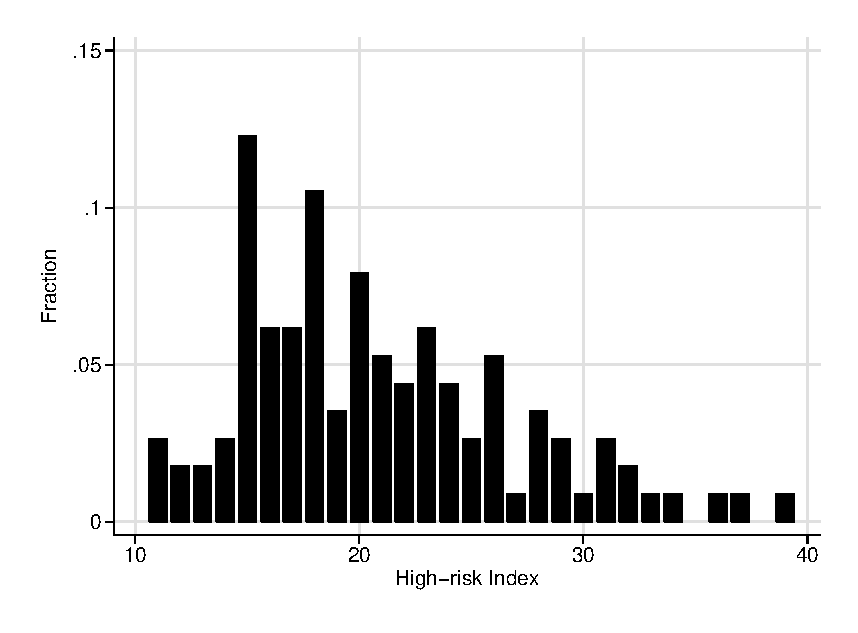
\includegraphics[width=.9\columnwidth]{output/abc_hri.eps}
\floatfoot{
\footnotesize
\noindent Note: This plot shows the distribution of the High-Risk Index (HRI) for ABC, which determined eligibility. Subjects were eligible if they had a score of 11 or more.}
	\end{figure}
\end{center}

\begin{center}
	\begin{figure}[H]
		\caption{High-Risk Index Distribution, CARE} \label{figure:hridistcare}
		\centering
		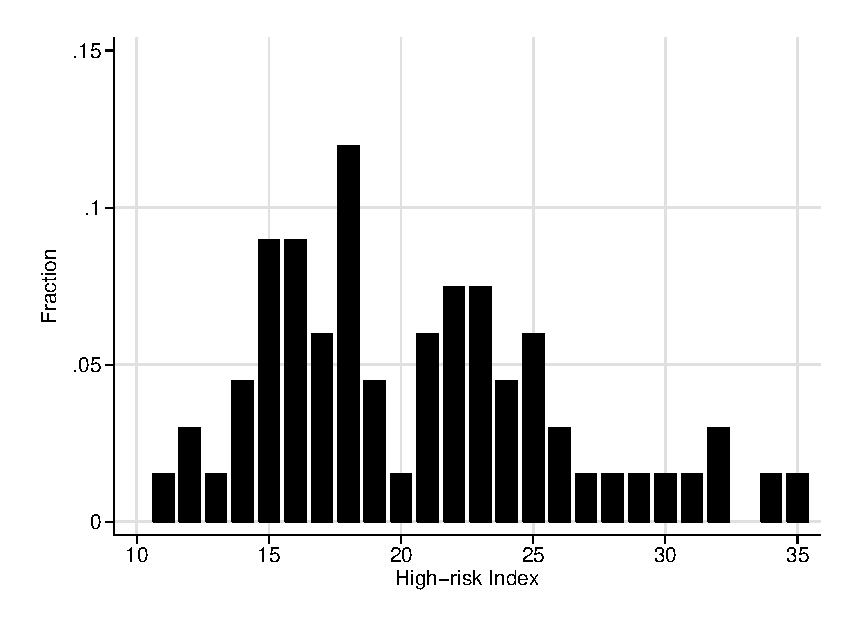
\includegraphics[width=.9\columnwidth]{output/care_hri.eps}
\floatfoot{
\footnotesize
\noindent Note: This plot shows the distribution of the High-Risk Index (HRI) for CARE, which determined eligibility. Subjects were eligible if they had a score of 11 or more.}
	\end{figure}
\end{center}

\noindent Figures~\ref{figure:hridistabc} and \ref{figure:hridistcare} display the distribution of the HRI score among all participants in ABC and CARE, respectively. All subjects were substantially disadvantaged. Maternal age when the target child was born was, on average, 19.9 years in ABC and 21.1 years in CARE. Approximately half of the mothers of both treatment and control group participants in ABC were 19 years or younger and one third were 17 years or younger. In CARE, approximately half of the mothers of both treatment and control group participants were 20 years or younger and one third were 17.2 years or younger.  Mean maternal IQ score in ABC was approximately 85, one standard deviation below the national mean. In CARE, the mean maternal IQ score was approximately 87. Only 25\% of the ABC subjects lived with both biological parents, and more than 50\% lived with extended families in multi-generational households (61\% of treatment-group subjects and 56\% of control-group subjects).\footnote{\citet{Ramey_Campbell_1991_childreninpoverty,Campbell_Ramey_1994_CD}.} About 79\% of subjects did not have a father in the home in both ABC and CARE. \\

\subsection{Randomization Protocol and Compromises} \label{appendix:randomization}

\noindent Randomization compromises throughout ABC's and CARE's implementations pose a challenge when evaluating the programs' effects. We discuss each case of compromise in detail in Section~\ref{section:background}. In Section~\ref{section:methodology},  we propose a methodology for adequately evaluating the programs while accounting for these compromises.

\begin{center}
	\begin{figure}[H]
		\caption{Randomization Protocol and Treatment Compliance, ABC} \label{fig:abc-flow}
		\centering
		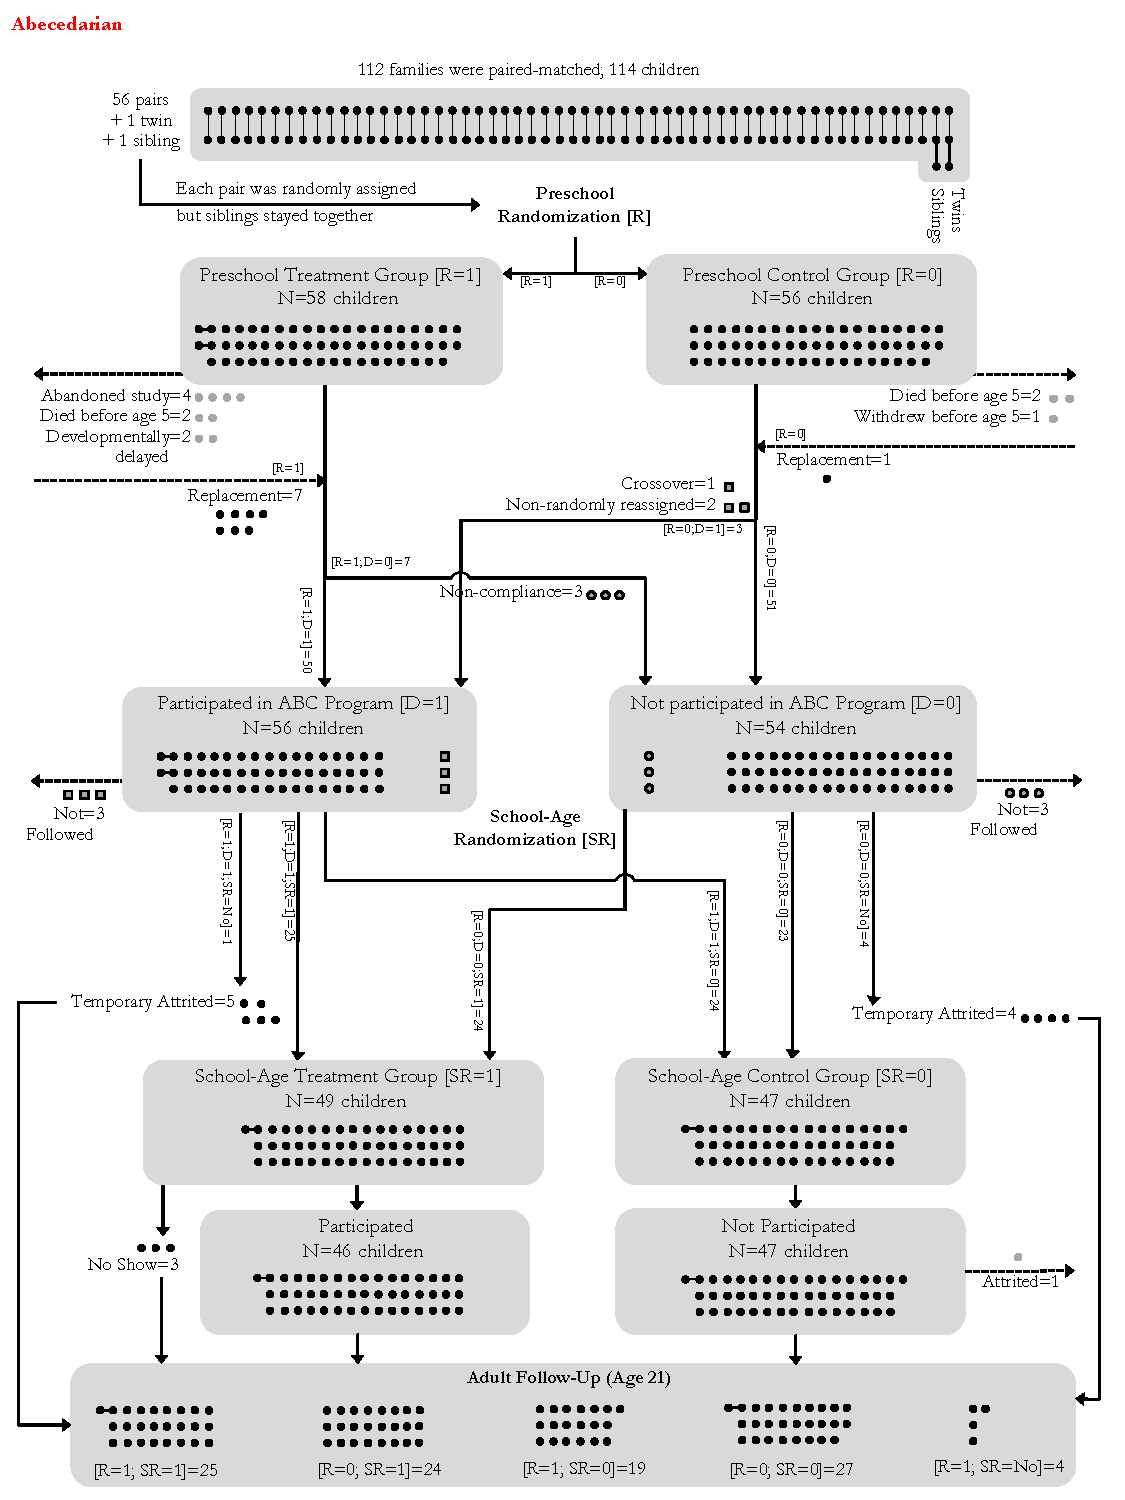
\includegraphics[width=.7\columnwidth]{output/abc_Diagram.pdf}
\floatfoot{
\footnotesize
\noindent
Sources: \cite{Ramey_Collier_etal_1976_CarolinaAbecedarianProject, Ramey_Smith_1977_AJMD,Ramey_Campbell_1979_SR,Ramey_Campbell_1984_AJMD}, internal documentation of the program, and own calculations. Note: The variable $R$ represents randomization into treatment, $[R=1]$, or control, $[R=0]$, groups. After the original randomization, some subjects died or withdrew from the program early in life and were replaced. $R$ also includes those replacements. Arrows pointing outside of the diagram indicate subjects who left the study permanently. The variable $P$ represents participation in the preschool-age program. The variable $SR$ represents randomization into the school-age program, $[SR=1]$, or out of it, $[SR=0]$. Some subjects were not randomized at school age, $[SR=No]$. We use the term ``temporarily attrited" for subjects who did not participate in the study at school age, but were later interviewed in the age-21 followup.
}
	\end{figure}
\end{center}

\begin{center}
	\begin{figure}[H]
		\caption{Randomization Protocol and Treatment Compliance, CARE} \label{fig:care-flow}
		\centering
		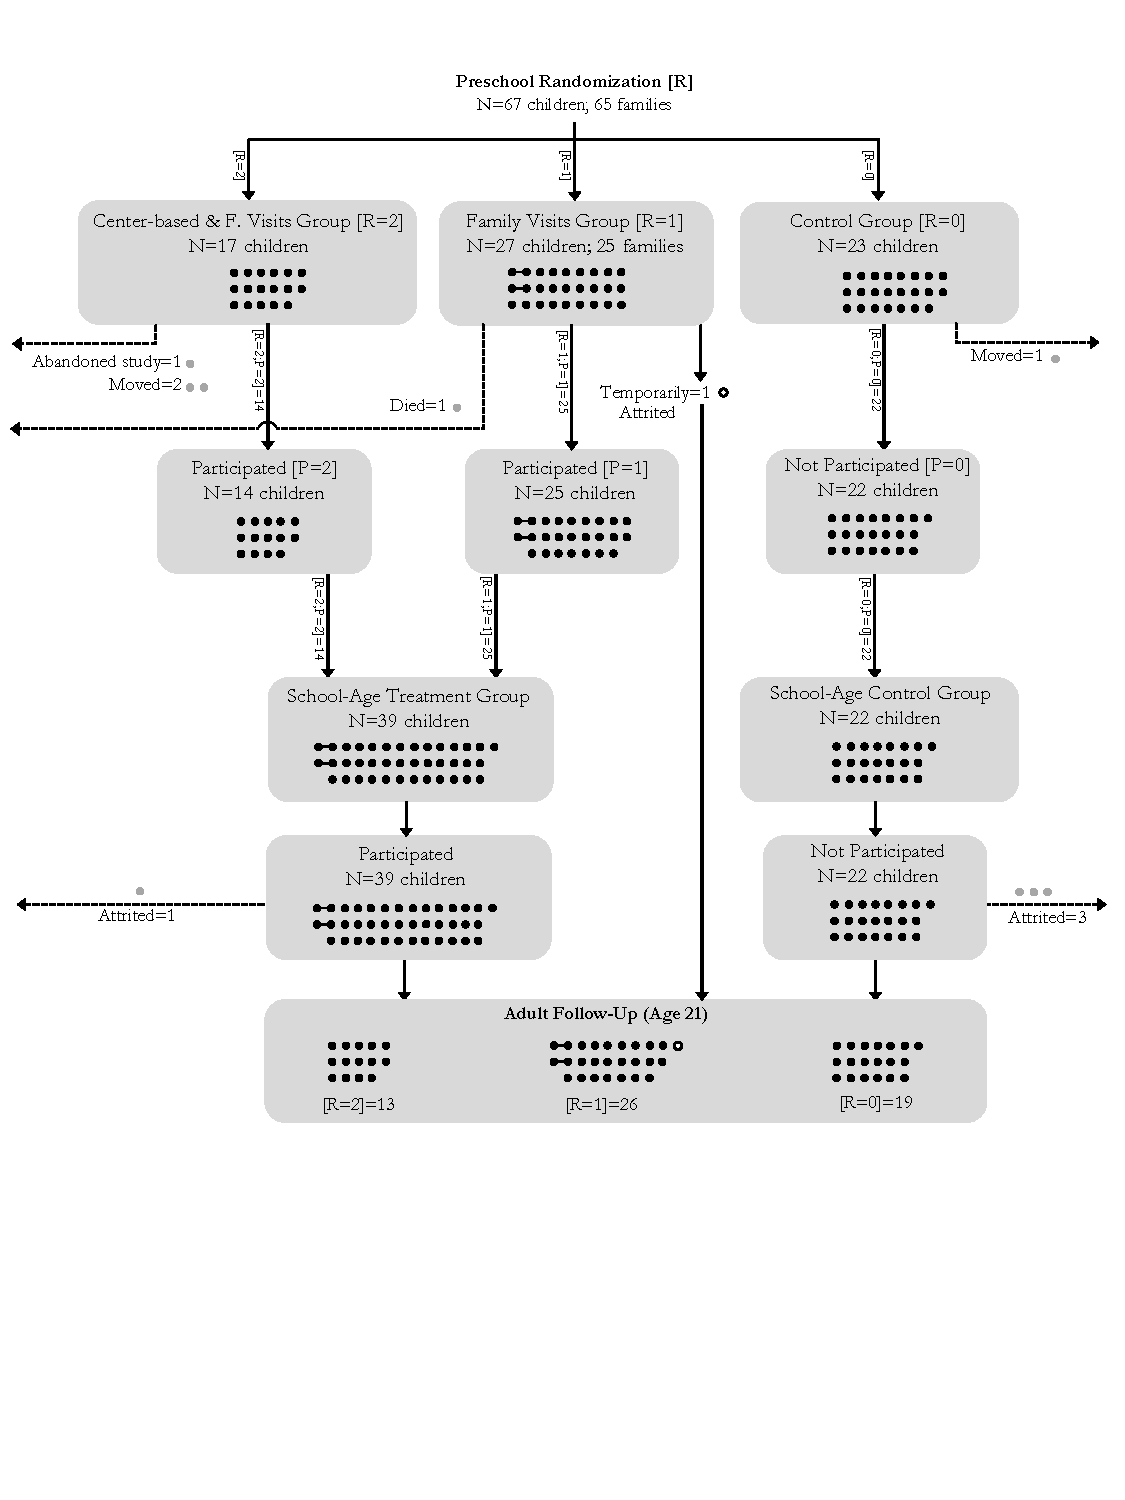
\includegraphics[width=.7\columnwidth]{output/care_Diagram.pdf}
\floatfoot{
\footnotesize
\noindent
Sources: \cite{Wasik_Ramey_etal_1990_CD}, internal documentation of the program, and own calculations. Note: The variable $R$ represents randomization into center-based preschool and family education, $[R=2]$, family education, $[R=1]$, or control, $[R=0]$. Arrows pointing outside of the diagram indicate subjects who left the study permanently. The variable $P$ represents participation in the corresponding group of the preschool-age program. The variable $SR$ represents those who participated in the school-age program, $[SR=1]$, or did not, $[SR=0]$. Unlike in ABC, there was no second-phase randomization in CARE. Rather, those in the center-based preschool and family education group and those in the family education group were automatically assigned to receive the school-age treatment. We use the term ``temporarily attrited" for subjects who did not participate in the study at school age, but were later interviewed in the age-21 followup.
}
	\end{figure}
\end{center}

\noindent Although most randomization compromises occurred at early stages, this methodology also accounts for the fact that a few individuals were not in the sample either for the second-phase randomization or for the adult-age follow-ups. In Appendix~\ref{appendix:data}, we describe the sample reductions that attrition at different stages of the study generates and test potential differences between the subjects who completed data follow-ups and the subjects who did not.\\

\subsection{Program Description and Content}

\subsubsection{Goals}
\noindent The original goals of treatment were to prevent mental retardation by enhancing overall development from birth,\footnote{Note that the clinical understanding of mental retardation was once associated with disadvantages that hindered early-life development \citep{Mental-Retardation_America_2004_BOOK_NYU}.} in turn fostering school-readiness for an at-risk population. Additional curriculum goals were to (i) support language, motor, and cognitive development; (ii) minimize high-risk behaviors; and (iii) develop socio-emotional competencies considered crucial for school success including task-orientation, emotional self-expression, independence, sharing, and cooperation.\footnote{\citet{Ramey_Collier_etal_1976_CarolinaAbecedarianProject, Ramey_etal_1985_Project-CARE_TiECSE, Sparling_1974_Synth_Edu_Infant_SPEECH, Wasik_Ramey_etal_1990_CD, Ramey-etal_2012-ABC}.} Implementation of ABC's and CARE's educational treatments evolved each successive year as program staff evaluated ongoing outcome data.\footnote{ \citet{Ramey-etal_1975_AJoMD, Finkelstein_1982_Day_Care_YC, McGinness_1982_Language-Poverty-Child,Haskins_1985_CD}.}\\


\subsubsection{Daily Schedule}
\noindent For both ABC and CARE, FPGC was open to families from 7:45 a.m. to 5:30 p.m., 5 days per week and 50 weeks per year.\footnote{\citet{Ramey_Collier_etal_1976_CarolinaAbecedarianProject, Ramey_etal_1985_Project-CARE_TiECSE}.} Subjects were offered free transportation to and from the center. A driver and second adult staffed each vehicle (one van and two station wagons) equipped with child safety seats.\footnote{\citet{Ramey_Campbell_1979_SR,abc2014-2015interviews}.} Data provided by FPGC indicate that approximately 65\% of treated ABC families utilized the free transportation.\footnote{\citet{Barnett_Masse_2002_benefitcost}.} Vehicles typically arrived by 9:00 a.m. to the center and departed around 3:45 p.m.\footnote{\citet{Ramey-et-al_1977_Intro-to-ABC}.} At FPGC, ABC and CARE treated subjects received breakfast, lunch, and a snack planned by a nutritionist.\footnote{ \citet{Haskins_1985_CD, Bryant_et_al_1987_Carolina_Approach_TIECSE, Ramey-et-al_1977_Intro-to-ABC}.} Infants received unlimited iron-fortified formula  until doctors advised adding solid food. The control-group subjects also received an unlimited amount of iron-fortified formula.\footnote{\citet{Campbell_Conti_etal_2014_EarlyChildhoodInvestments,abc2014-2015interviews}.} Meals were catered for ABC and CARE subjects by off-site kitchens. \\

\subsubsection{Program Staff and Physical Space}
\noindent To promote trust in FPGC within the sample families, staff were recruited from the local community.\footnote{\citet{Ramey-et-al_1977_Intro-to-ABC, Bryant_et_al_1987_Carolina_Approach_TIECSE, Feagans_1996_Childrens-Talk,abc2014-2015interviews}.} Infant and toddler caregivers as well as preschoool teachers demonstrated varied educational backgrounds ranging from high school graduation to master's degrees. Their average professional working experience with young children was 7 years.\footnote{\citet{Ramey_McGinness_etal_1982_Abecedarianapproach, Ramey_etal_1985_Project-CARE_TiECSE, Wasik_Ramey_etal_1990_CD}.}. All classroom staff participated in extensive training and were closely observed by FPGC's academic staff, as part of a broad variety of ongoing clinical and social research related to early childhood education, psychology, and health. In ABC, child-caregiver ratios varied by age: 3:1 for subjects up to 13 to 15 months of age; 4:1 for subjects up to 36 months; and 5:1 or 6:1 for subjects aged 3 to 5 years, depending on cohort size.\footnote{\citet{Ramey-et-al_1977_Intro-to-ABC,Ramey_Campbell_1979_SR,Ramey_McGinness_etal_1982_Abecedarianapproach}.} Child-caregiver ratios were similar in CARE.\footnote{\citet{Burchinal_Campbell_etal_1997_CD, Ramey_etal_1985_Project-CARE_TiECSE}}\\

\noindent The ABC and CARE staff included a program director, a secretary, 12 to 14 teachers and assistant teachers, 3 administrative staff members, and a transportation supervisor.\footnote{\citet{Ramey-et-al_1977_Intro-to-ABC,Ramey_McGinness_etal_1982_Abecedarianapproach, Bryant_et_al_1987_Carolina_Approach_TIECSE}.} Teacher aides, recruited from the local community, held high school diplomas (at minimum) and were comparatively well-compensated in the preschool field. They remained a stable treatment component throughout the study. Classroom staff received weekly training, daily supervision, and frequent professional development from outside consultants.\footnote{\citet{Obrien-Sanders_1974_ABC-brochure, Ramey_etal_1985_Project-CARE_TiECSE, Sanders-Stokes_1979_Status-Report,Klein-Sanders_1982_Status-Report,abc2014-2015interviews}.}\\

\noindent Infant nurseries, toddler rooms, and preschool classrooms were housed on different floors of FPGC. Early reports indicate that FPGC allocated two floors to ABC, but later reports indicate the use of three floors.\footnote{\citet{Ramey_Smith_1977_AJMD,Ramey_Campbell_1979_SR,Ramey_1981_Modification}.} Two infant nurseries were staffed by five adults in a suite of four adjoining rooms: two sleeping rooms contained seven cribs each, while the other two rooms were designated for activities.\footnote{ \citet{Ramey-et-al_1977_Intro-to-ABC}.} The four rooms opened into a large, shared space with feeding tables, an area for food preparation, and a couch.\footnote{\citet{Ramey_Campbell_1979_SR}.} Offices for the medical staff, along with two examining rooms and facilities for laboratory tests were located around the corner from the infant nurseries.\footnote{\citet{abc2014-2015interviews}.} Two multi-age toddler rooms were located one floor below the infant nurseries. One room served subjects who were 1 to 2 years old and the other served subjects 2 to 3 years old.\footnote{\citet{Ramey_Smith_1977_AJMD,Ramey_Campbell_1979_SR}.} 3-year-olds were housed in a closed classroom near the toddler rooms. On the lowest floor, 4-year-olds shared an open classroom with a public kindergarten program; the two classes were separated by a long, low bookcase. This information is not available for CARE to the best of the authors' knowledge. FPGC offered two outdoor play areas for both ABC and CARE: one for subjects up to age 3, and the other for older subjects.\footnote{\citet{Ramey_Campbell_1979_SR,Ramey_McGinness_etal_1982_Abecedarianapproach}.}\\

\subsubsection{Approach to Child Development}
%Direct from the paper
\noindent Curriculum delivery enabled a highly customized learning experience for treated subjects in both ABC and CARE. Infant caregivers recorded subject observations on progress charts and collaborated with FPGC's curriculum developers and academic researchers to rotate learning activities every 2 to 3 weeks for each treated subject.\footnote{\citet{Ramey_Collier_etal_1976_CarolinaAbecedarianProject,Campbell_Ramey_1994_CD}.} Preschool rooms featured intentionally organized environments to promote pre-literacy and access to a rich set of learning tools. The full-day curriculum emphasized active learning experiences, dramatic play, and pre-academics. Frequent 1:1 or 2:1 child-adult interactions prioritized language development for social competence. For ages 3 through 5, as the cohorts approached public school entry, classroom experiences were increasingly structured  towards the development of pre-academic skills and ``socio-linguistic and communicative competence.''\footnote{\citet{Ramey-et-al_1977_Intro-to-ABC, Haskins_1985_CD, Ramey_1981_Modification, Ramey_Campbell_1979_SR, Ramey_Smith_1977_AJMD, Ramey_McGinness_etal_1982_Abecedarianapproach, Sparling_Lewis_1979_BOOKLearninggamesFirstThree,Sparling_Lewis_1984_BOOKLearningGamesThreesFours}.} In CARE, FPGC offered a summer program before the start of kindergarten designed to target specific skills to ensure success in a kindergarten classroom (e.g., lining up when exiting the classroom). This program was available to subjects in both the center-based preschool and family education group and the family education group.\footnote{\citet{Ramey_etal_1985_Project-CARE_TiECSE}.} \\

\noindent ABC's and CARE's learning programs were influenced by key developmental theorists, including Bowlby, Piaget, Vygotsky, and Tough.\footnote{\citet{Sparling_1974_Synth_Edu_Infant_SPEECH,Mcginness_1981_Developing,abc2014-2015interviews}.} All four ABC cohorts and two CARE cohorts participated in curriculum developers Sparling and Lewis' ``Learningames for the First Three Years.''\footnote{ \citet{Sparling_Lewis_1979_BOOKLearninggamesFirstThree}.} The ``Learningames'' were implemented daily by infant and toddler caregivers in 1:1 child-adult interactions. Each ``Learningames'' activity stated a developmentally-appropriate objective, the necessary materials, directions for teacher behavior, and expected subject outcome. The activities were designed for use both indoors and outdoors, while dressing, eating, bathing, or during play.\footnote{\citet{Ramey_Campbell_1979_SR, Ramey_1981_Modification,Sparling_Lewis_1979_BOOKLearninggamesFirstThree}.}\\

\noindent Supplemental curricula for preschool rooms varied throughout the study, and included ``Cook and Learn,'' ``Bridges to Reading,'' ``Peabody Early Experiences Kit,'' ``GOAL Math Program,'' ``My Friends and Me,'' and ``Teaching all Children to Read.''\footnote{ \citet{Greenberg_Epstein_1973_BOOKBridgestoreading,Karnes1973,Dunn_Chun_etal_1976_BOOKPeabodyearlyeducation,Davis_1977_BOOKMyfriends,Wallach_1976_Teaching-All-Children}.} Packaged preschool supplemental curricula supported individual subjects' learning needs, and varied from year to year.\footnote{ \citet{Ramey_McGinness_etal_1982_Abecedarianapproach,Mcginness_1981_Developing,Finkelstein_1982_Day_Care_YC,Wasik_Ramey_etal_1990_CD}.}\\
%SK notes to co-authors: I'm currently waiting for info from Lynne Vernon-Feagans to potentially include a social worker to the list of staff!

\noindent Subjects in CARE randomized into the center-based preschool and family education group or the family education group also received home visits. These visits were designed to transmit information on child development and skills involved with parenting including strategies for parent-child interactions based on ``Learningames" activities and problem-solving techniques.\footnote{\citet{Bryant_et_al_1987_Carolina_Approach_TIECSE, Wasik_Ramey_etal_1990_CD, Burchinal_Campbell_etal_1997_CD}} Home visitors were trained to ensure they were capable to form a strong relationship with the parent and successfully implement the curriculum.\footnote{\citet{Bryant_et_al_1987_Carolina_Approach_TIECSE}} The visits lasted about an hour, and occurred weekly until the subject was 3 years old. After age 3, the home visits were less frequent and depended on the preferences of the parents. They were usually about once a month after age 3.\footnote{\citet{Bryant_et_al_1987_Carolina_Approach_TIECSE, Wasik_Ramey_etal_1990_CD, Burchinal_Campbell_etal_1997_CD}} 

\subsubsection{Medical Care and Nutrition}
%Direct from the paper
ABC and CARE provided comprehensive on-site medical care because they were conducted in conjunction with a longitudinal medical research study on infectious respiratory diseases in group environments.\footnote{\citet{Henderson-et-al_1982_NEJoM}.} Treatment group subjects were monitored daily for signs of illness. All treated subjects received medical care while attending center-based preschool; the first ABC cohort of control-group subjects also received medical care during the program's first year of implementation.\footnote{\citet{Ramey_Collier_etal_1976_CarolinaAbecedarianProject, Bryant_et_al_1987_Carolina_Approach_TIECSE, Ramey_Campbell_1991_childreninpoverty,Campbell_Ramey_1994_CD}.}$^{,}$\footnote{Subjects in both the treatment and control groups of the first cohort received free medical care provided by ABC. The control group of the first cohort only received medical care in the first year of the program; the treatment group of the first cohort received medical care for all years of the program. In the subsequent cohorts, only subjects in the treatment group received free medical care provided by ABC. Both CARE cohorts of treated subjects received medical care.}\\
%Direct from the paper

\noindent In ABC, primary pediatric care was provided by a family nurse practitioner and a licensed practical nurse, both under the supervision of one pediatrician who was on continuous duty at the center.\footnote{\citet{Haskins-et-al_1978_JoPP}.} In CARE, the medical staff included two pediatricians, a family nurse practitioner, and a licensed practical nurse.\footnote{\citet{Bryant_et_al_1987_Carolina_Approach_TIECSE}.} The medical staff provided regularly scheduled check-ups, immunizations, parental counseling, and initial assessment of illnesses.\footnote{\citet{Ramey-et-al_1977_Intro-to-ABC, Bryant_et_al_1987_Carolina_Approach_TIECSE}.} The CARE treatment group received standard check-ups when they were 2, 4, 6, 9, 12, 18, and 24 months old and annually thereafter. While in treatment, they also received the standard immunizations.\footnote{\citet{Bryant_et_al_1987_Carolina_Approach_TIECSE, Campbell_Conti_etal_2014_EarlyChildhoodInvestments}.} In ABC, a licensed practical nurse visited classrooms for up to two hours on a daily basis to monitor the subjects' health status.\footnote{\citet{Sanyal_Henderson_etal_1980_JoPediatrics}.} Although this medical care was offered to the treatment-group families free of charge, it was the policy of the medical staff to refer families to a community hospital for serious treatment. While ABC and CARE provided aspirin, immunizations, and basic medicines, families were responsible for purchasing any prescription medication subjects required. There is no data currently available on treatment received for serious conditions or use of prescription medication.  \\

\noindent Infants were supplied with iron-fortified formula. Subjects older than 15 months of age were provided breakfast, lunch, and an
afternoon snack all planned by a nutritionist.\footnote{\citet{Bryant_et_al_1987_Carolina_Approach_TIECSE, Campbell_Conti_etal_2014_EarlyChildhoodInvestments,abc2014-2015interviews}.} Control families received diapers for up to three years and unlimited iron-fortified bottled formula through 15 months.\footnote{\citet{Ramey_Collier_etal_1976_CarolinaAbecedarianProject,Ramey_Campbell_1979_SR, Ramey_etal_1985_Project-CARE_TiECSE}.}

\subsubsection{School-age Treatment}

\noindent The ABC participants were subject to a second-phase randomization into a school-age treatment (95 subjects continued to this stage of treatment). The CARE participants in the center-based preschool and family education group and the family education group received the school-age treatment without randomization. The school-age treatment lasted for the first three years of elementary school and consisted of home visits conducted by a Home/School Resource Teacher.\footnote{\cite{Burchinal_Campbell_etal_1997_CD}.} These visits were structured to increase exposure to reading and mathematics and promote parental involvement in the academic process.\\

\noindent The curriculum was delivered through sets of activities (around 60 per year) that developed skills such as handwriting, phonics, and math facts.\footnote{\cite{Campbell-Ramey_1989_Preschool-vs-School-age}.} Teachers worked to encourage parental involvement in the subject's academics and provided incentives to families to comply with the treatment, such as giving gift certificates to restaurants and books for children upon the completion of activity packets. Home activities were designed at the appropriate level to promote success.\\

\noindent Teachers had graduate-level education, training in special education, \textit{or} were qualified to act as consultants for in-school teachers to address any problems that arose.\footnote{\cite{Ramey_Campbell_1991_childreninpoverty}.} They met with parents every other week to deliver new activities for them to complete with their children and discuss the child's level of success with the previous set of activities. In addition, teachers helped parents with issues such as adult literacy, housing, and medical care. Thus, the teacher had a dual role as a parent educator and an advocate for the child in their educational institution.

\subsection{Treatment Substitution}

\noindent In ABC, the families of almost $70\%$ of the control-group subjects enrolled their children in high-quality preschools. In CARE, $74\%$ of families in the control group and $62\%$ of families in the family education group enrolled their children in high-quality preschools. We refer to this phenomenon as treatment substitution; accounting for it is fundamental when evaluating the program, as we argue in Section~\ref{section:methodology}. In this appendix, we thoroughly describe the characteristics and costs of the preschool centers providing alternative treatment, in order to create a comparison with the treatments offered by ABC and CARE.\\

\noindent Most of the families in the ABC and CARE control groups enrolled their children in alternative preschools that received federal subsidies and, therefore, were regulated by the Federal Interagency of Day Care Requirements (FIDCR). Figure~\ref{fig:ccabc} and Figure~\ref{fig:cccare} show the amount of enrollment into subsidized and non-subsidized care for ABC and CARE, respectively. Subsidized centers were required to have trained staff who were able to implement curricula designed to enhance cognitive, social, and linguistic competence in disadvantaged children.\footnote{\citet{Burchinal_etal_1989_CD_Daycare-Pre-K-Dev}.} Thus, we consider these centers to offer high-quality center-based preschools.

\begin{center}
	\begin{figure}[H]
		\caption{Treatment Substitution, ABC} \label{fig:ccabc}
		\centering
		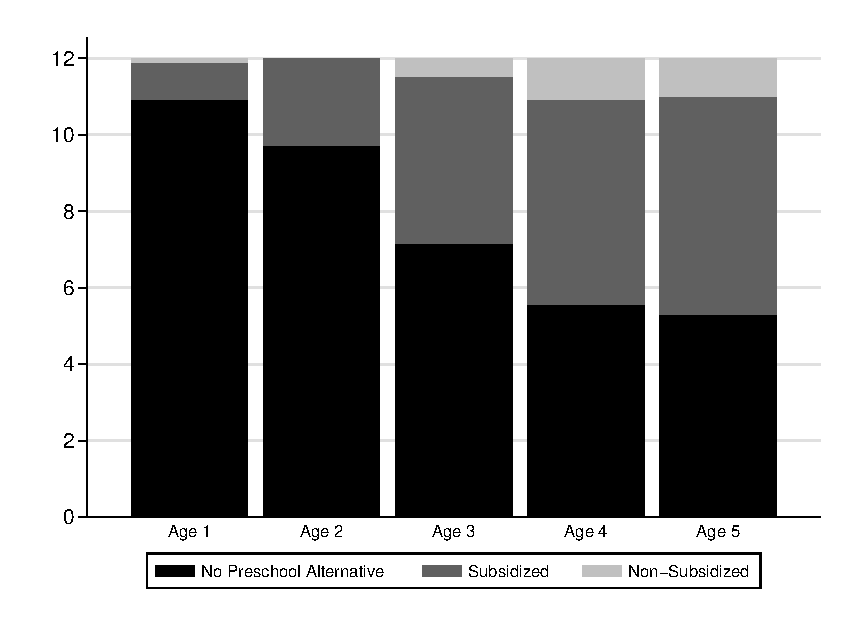
\includegraphics[width=.9\columnwidth]{output/blackwhite_CCnumber.eps}
\floatfoot{
\footnotesize
\noindent Note: This figure describes the take-up of center-based preschool by families in the ABC control group. The vertical axis represents the average number of months per year the subjects of the control group spent in center-based preschool. Subsidized centers were highly regulated and, therefore, high-quality. Non-subsidized preschool services were center-based but not regulated. Other sources of preschool could have included care by parents, relatives, or non-relatives.}
	\end{figure}
\end{center}

\begin{center}
	\begin{figure}[H]
		\caption{Treatment Substitution, CARE} \label{fig:cccare}
		\centering
		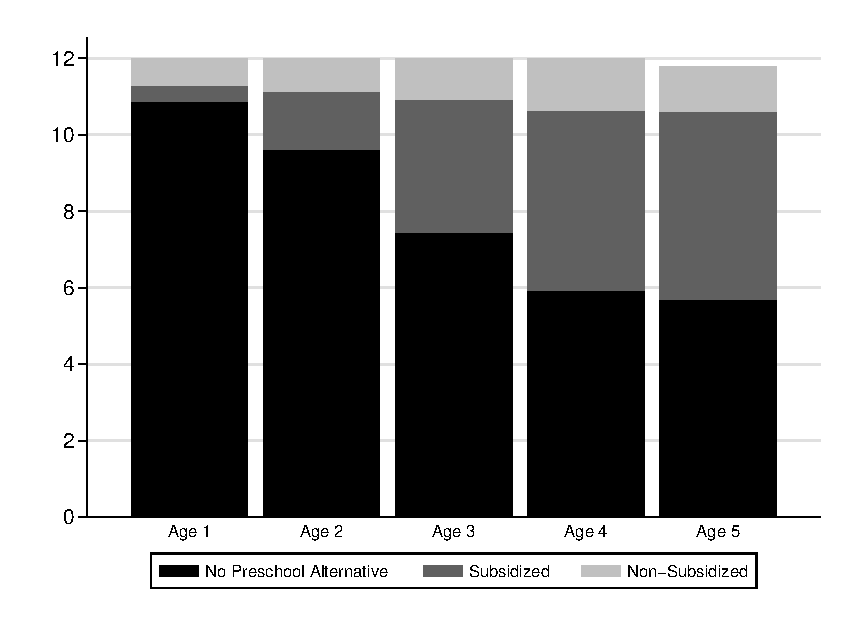
\includegraphics[width=.9\columnwidth]{output/blackwhite_CCnumber_care.eps}
\floatfoot{
\footnotesize
\noindent Note: This figure describes the take-up of center-based preschool by families in the CARE family education and control groups. The vertical axis represents the average number of months per year the subjects of the control group spent in center-based preschool. Subsidized centers were highly regulated and, therefore, high-quality. Non-subsidized preschool services were center-based but not regulated. Other sources of preschool could have included care by parents, relatives, or non-relatives.}
	\end{figure}
\end{center}


\subsubsection{Regulation}

\noindent During the ABC and CARE programs, North Carolina had an active, high-quality system of public preschools for vulnerable families funded by several public programs. Examples include Title IV-A of the Social Service Administration (SSA), Aid to Families with Dependent Children (AFDC), and Title IV-B of Child Welfare Services. These funding efforts were amplified in 1975 by Title XX of the SSA, Social Services Block Grant, which was the main federal source of preschool financing in the US when ABC was active.\footnote{\citet{Robins_1988_Federal-Child-Care}.}\\

\noindent Federally funded preschool services were regulated according to FIDCR standards, which defined stringent regulation for center-based programs for children between the ages of 3 and 6.\footnote{\citet{Department-of-Health_1968_DayCareRequirements}.} These requirements were enforced and preschool providers were aware of them.\footnote{\citet{Kuperman_2015_Clifford-Russell-Interview}.} Additionally, North Carolina had a mandatory licensing law for preschool facilities. This regulation only applied to centers serving subjects below the age of 3 while FIDCR applied to centers for older subjects (between the ages of 3 and 6). The relative weakness of this regulation is not very relevant for our study because treatment substitution occurred mostly after age 3.\footnote{\citet{NCGA_1971_House-Bill-100}.} Table~\ref{table:staff} compares a widely-used quality standard, the child-staff ratio, between the North Carolina and FIDCR standards and the actual ABC and CARE numbers.

%Not in main paper
\begin{table}[H]
\caption{Child-Staff Ratios for North Carolina, FIDCR, and Actual ABC and CARE Ratios}
\label{table:staff}
\begin{threeparttable}
\begin{tabular}{lccc}
\hline \hline
 &NC Standards & FIDCR &  ABC and   \\
Age	& Level I &  Standards  & CARE Ratios\\ \hline
0--1	& 6:1*	&  				& 	3:1					\\
1--2	& 8:1* 	& 				&   4-5:1				\\
2--3	& 12:1* & 				& 	4-5:1				\\
3--4	& 15:1 	& 		5:1*	& 	4-5:1 				\\
4--5	& 20:1 	& 		7:1*	& 	5-6:1 				\\
5--6 & 25:1  &		7:1*	&	5-6:1				\\
\hline \hline
\end{tabular}
\begin{tablenotes}
\footnotesize
Sources: \cite{Department-of-Health_1968_DayCareRequirements,NCGA_1971_House-Bill-100,Ramey-et-al_1977_Intro-to-ABC,Ramey_Campbell_1979_SR,Ramey_McGinness_etal_1982_Abecedarianapproach, Burchinal_Campbell_etal_1997_CD}.\\
Note: The starred ratios represent the ones we believe were the most relevant for ABC control-group subjects and CARE control-group and family-education-group subjects.
\end{tablenotes}
\end{threeparttable}
\end{table}

\subsubsection{Costs}

\noindent Center-based preschool centers had a uniform rate for subsidy-eligible children, independent of which program the children were eligible for. This was mandated by the County Department of Social Services. The most common way for a child to be eligible was by belonging to a poor family with either a single mother who worked or studied, or with both parents who either worked or studied. Other conditions, such as abuse risk, were also considered. Information on the subsidy rates paid is limited, but evidence from 1982 records indicates that at that time, the subsidy value for full-time center-based preschool was between \$59 and \$111 (2014 USD) per week.\footnote{\citet{ReportNCGenAssembly_DayCare_1983}.} 

\subsection{Data} \label{appendix:data}

In Table~\ref{tab:ecvars_1} through Table~\ref{tab:adultvars_2}, we summarize the data availability for both ABC and CARE. The data collection processes in both programs were analogous by design. For both programs, the treatment and control groups were followed into adulthood with relatively low attrition. For ABC, subjects were followed annually through elementary school and at ages 12, 15, 21, and 30. Health and administrative crime data were collected when the subjects reached their mid-30s. For CARE, the exact same follow-ups are available with the exception of the age 15 follow-up.\\

\begin{sidewaystable}[H]
\small
\caption{Early Childhood Data (Part I)}
\label{tab:ecvars_1}
\centering
\begin{adjustbox}{max width=\textwidth, max height=\textheight,keepaspectratio}
\begin{threeparttable}
\tiny
\begin{tabular}{L{3cm} C{3.5cm} C{4cm} C{1.5cm} C{1.5cm}  C{6cm}}
\toprule
\textbf{Category}	&	\textbf{Sub-Category}	&	\textbf{Description}	&	\textbf{ABC Age}  	&  \textbf{CARE Age}  & 	\textbf{Measure}	\\ \midrule
Demographics	&	Gender	&	Gender of child	&	Birth, 18, 30, 42, 54	&	 Birth, 18, 30, 42, 54	&	Demographic Interview	\\
	&	\\
	&	Race	&	Race/Cultural identity of child	&	Birth, 18, 30, 42, 54	&	 Birth, 18, 30, 42, 54	&	 Demographic Interview\\
	&	\\
	&	Birth Date	&	Date of birth of child	&	Birth, 18, 30, 42, 54	& 	Birth, 18, 30, 42, 54	&	 Demographic Interview	\\ \midrule
Cognitive Assessments	&	Language Ability	&	Auditory association, Verbal expression, etc. 	&	36, 42, 48, 54	&	30, 42, 54	&	ITPA$^{ABC}$, GPB$^{ABC}$, PLP$^{ABC}$, MSCD \\
	&	\\
	&	Intelligence Levels	&	SBIS 	&	24, 36, 48, 60	&	24, 36, 48, 60	&	SBIS	\\
	&		&	WPPSI	&	60	&	60	&	WPPSI	\\
	&		&	BSID 	&	3, 6, 9, 12, 18, 24	&	6, 12, 18, 24		&	BSID	\\
	&		&	UOSPD	&	15	&	- 	&	UOSPD$^{ABC}$	\\
	&		&	RPM	&	60	&	-	&	RPM$^{ABC}$	\\
	&	\\
	&	Quantitative	 &	BSID 	&	3, 6, 9, 12, 18, 24	&	6, 12, 18, 24		&	BSID	\\
	&		&	MSCD 	&	30, 42, 54		&	30, 42, 54	&	MSCD	\\
	&	\\
	&	Memory	&	BSID 	&	3, 6, 9, 12, 18, 24	& 	6, 12, 18, 24		&	BSID	\\
	&		&	MSCD 	&	30, 42, 54	&	30, 42, 54	&	MSCD	\\
	&	\\
	&	Motor Development	&	BSID 	&	3, 6, 9, 12, 18, 24	&	6, 12, 18, 24		&	BSID\\
	&		&	MSCD 	&	30, 42, 54	&	30, 42, 54	&	MSCD	\\
	& 	\\
	&	Critical Thinking	&	Curiosity	&	30, 36, 42, 48, 54, 60, 66, 72	& - &	Infant Behavior Inventory$^{ABC}$	\\ \midrule
Non-Cognitive Assessments	&	Social Skills	&	Positive social response	&	30, 36, 42, 48, 54, 60, 66, 72	&	6, 12, 18, 24		&	Infant Behavior Inventory$^{ABC}$, Bayley Infant Inventory$^{CARE}$	\\
	&		&	Creativity	&	30, 36, 42, 48, 54, 60, 66, 72	&	- 	&	Infant Behavior Inventory$^{ABC}$	\\
	&	\\
	&	Self-Control	&	Locus of control	&	3, 18	&	6, 18	& 	RIES	\\
	&		&	Distractibility, Attentiveness	&	30, 36, 42, 48, 54, 60, 66, 72	&	6, 12, 18, 24		&	Infant Behavior Inventory$^{ABC}$, Bayley Infant Inventory$^{CARE}$	\\
	&	\\
	&	Emotional Health	&	KRT	&	24, 36, 48, 60	&	24, 30, 36, 42, 48, 60	&	KRT	\\
	&	\\
	&	Self-Consciousness	&	Self-consciousness	&	30, 36, 42, 48, 54, 60, 66, 72	&	-	&	Infant Behavior Inventory$^{ABC}$	\\
\bottomrule
\end{tabular}
\begin{tablenotes}
\scriptsize
\item Sources: Authors' description. \\	
\item Note: This table describes the major categories of variables that were measured for ABC and CARE subjects up to age 6. ABC and CARE ages are measured in months. This is not an exhaustive list of variables, nor does it include variables from auxiliary data. Instruments or questionnaires available for only one of the studies are indicated with the superscript $^{ABC}$ or $^{CARE}$.  \textbf{Abbreviations are as follows.} ITPA: Illinois Test of Psycholinguistic Ability. GPB: Gordon Psycholinguistic Battery. PLP: Preschool Language Performance. MSCD: McCarthy Scales of Children's Development. BSID: Bayley Scales of Infant Development and Infant Behavior. UOSPD: Uzgiris-Hunt Ordinal Scales of Psychological Development. RPM: Raven's Progressive Matrices. RIES: Rotter's Internality-Externality Scale. KRT: Kohn and Rosman Test Behavior Inventory.
\end{tablenotes}
\end{threeparttable}
\end{adjustbox}
\end{sidewaystable}




\begin{sidewaystable}[H]
\small
\caption{Early Childhood Data (Part II)}
\label{tab:ecvars_2}
\centering
\begin{adjustbox}{max width=\textwidth, max height=\textheight,keepaspectratio}
\begin{threeparttable}
\tiny
\begin{tabular}{L{3cm} C{3.5cm} C{4cm} C{1.5cm} C{1.5cm}  C{6cm}}
\toprule
\textbf{Category}	&	\textbf{Sub-Category}	&	\textbf{Description}	&	\textbf{ABC Age}  	&  \textbf{CARE Age}  & 	\textbf{Measure}	\\ \midrule
Family Environment	&	Family Members	&	Number of primary caretakers	&	Birth, 18, 30, 42, 54	&	18, 30, 42, 54, 60	&	Demographic Interview	\\
	&		&	Relationship with family members, including father, mother, siblings, etc.	&	Birth, 18, 30, 42, 54	&	18, 30, 42, 54, 60	&	Demographic Interview	\\
	&		&	Number of siblings	&	Birth, 18, 30, 42, 54	&	Birth, 18, 30, 42, 54, 60	&	Demographic Interview	\\
	&		&	Marital status of parents	&	Birth, 18, 30, 42, 54	&	Birth, 18, 30, 42, 54, 60	&	Demographic Interview	\\
	&		&	Marital conflicts between parents	&	6, 18	&	Birth, 6, 18, 36	&	Demographic Interview$^{CARE}$, Parental Attitudes Research Inventory	\\
	&		& Father at home & 18, 30, 42, 54  & 18, 30, 42, 54, 60 & Demographic Interview \\
	&	\\
	&	Family Economic Environment	&	Parents' occupation	&	Birth, 18, 30, 42, 54	& 	Birth, 18, 30, 42, 54, 60		&	Demographic Interview	\\
	&								& Mother works & 18, 30, 42, 54 & 18, 30, 42, 54, 60 & Demographic Interview \\
	&		&	Source of child support	&	Birth, 18, 30, 42, 54	&	18, 30, 42, 54, 60	&	Demographic Interview	\\
	&		&	Family income	&	Birth, 18, 30, 42, 54	&	Birth, 18, 30, 42, 54, 60	&	Demographic Interview	\\
	&	\\
	&	Parents and Home Environment & Parents' authority, warmth, family conflict, etc. & 6, 18, 30, 42, 54 & 6, 12, 18, 30, 42, 54 & Parent Interview \\
	&	\\
	&	Family Social Status	&	Parents' education background	&	Birth, 18, 30, 42, 54	&	Birth, 18, 30, 42, 54, 60		&	Demographic Interview	\\
	&		&	Risk taking of family members	&	Birth	&	- 	&	Parent Interview$^{ABC}$	\\
	&	\\
	&	Family Members' Physical Health	&	Health issues of parents	&	Birth	&	Birth	&	Parent Interview	\\
	&		&	Pregnancy history	&	Birth	&	Birth	&	Parent Interview	\\ \midrule
Childcare	&	Day-care Experience	&	Time and location of day-care, Age when begin	&	Birth, 18, 30, 42, 54	&	18, 30, 42, 54	&	Demographic Interview	\\
			&						& 	Home visits &	-	&	6, 18, 30, 42, 54, 60	& Home Visit Data$^{CARE}$ \\
	&	\\
	&	Parental Care	&	Maternal warmth, Maternal involvement with child	&	6, 18, 30, 42, 54	&	6, 12, 18, 30, 42, 54	&	Home Stimulation	\\
	&		&	Provision of appropriate play materials	&	6, 18, 30, 42, 54	&	 6, 12, 18, 30, 42, 54	&	Home Stimulation	\\
	&		&	Avoidance of restriction and punishment	&	6, 18, 30, 42, 54	&	6, 12, 18, 30		&	Home Stimulation	\\
	&		&	Authoritarian control	&	6, 18, 30, 42, 54	&	6, 12, 18, 30, 36, 42, 102		&	Home Stimulation, Parental Attitudes Research Inventory	\\
	&		&	Democratic attitudes	&	6, 18	&	6, 18, 36	&	Parental Attitudes Research Inventory	\\
	&		&	Hostility and rejection	&	6, 18	&	6, 18, 36	&	Parental Attitudes Research Inventory	\\
	&		&	Parents' knowledge of childcare	&	Birth	&	-	&	Parent Interview$^{ABC}$	\\ \midrule
Physical Health	&	Growth Data	&	Height, Weight, Head circumference, etc.	&	3, 6, 9, 12, 18, 24, 36, 48, 60	&	Birth, 6, 12, 18, 24, 36, 48, 60	&	Growth Measures	\\
\bottomrule
\end{tabular}
\begin{tablenotes}
\scriptsize
\item Sources: Authors' description. \\	
\item Note: This table describes the major categories of variables that were measured for ABC and CARE subjects up to age 6. ABC and CARE ages are measured in months. This is not an exhaustive list of variables, nor does it include variables from auxiliary data.  Instruments or questionnaires available for only one of the studies are indicated with the superscript $^{ABC}$ or $^{CARE}$.
\end{tablenotes}
\end{threeparttable}
\end{adjustbox}
\end{sidewaystable}



\begin{sidewaystable}[H]
\begin{threeparttable}
\small
\caption{Childhood and Adolescence Data (Part I)} \label{tab:youthvars_1}
\centering
\tiny	
\begin{tabular}{L{3.5cm} C{3.5cm} C{5cm} C{1.5cm} C{1.5cm} C{6cm}}
\toprule
\textbf{Category}	&	\textbf{Sub-Category}	&	\textbf{Description}	&	\textbf{ABC Age}  	&  \textbf{CARE Age}  & 	\textbf{Measure}	\\ \midrule
Cognitive Assessment	&	Language Ability	&	Adaptive Language Inventory	&	6, 7, 8	&	6, 7, 8	&	Adaptive Language Inventory	\\
	&		&	Language Questionnaire	&	12	&	- 	&	Language Questionnaire$^{ABC}$	\\
	&		&	MSCD 	&	7	&	- 	&	MSCD$^{ABC}$	\\
	&	\\
	&	Intelligence Tests	&	SBIS	 &	6	&	7	&	SBIS	\\
	&		&	 WIS	&	6, 7, 8, 12, 15	&	6, 8	&	WIS	\\
	&		& Kaufman$^{CARE}$ & 	-	& 6 & Kaufman$^{CARE}$ \\
	&	\\
	&	Quantitative Skills	&	MSCD$^{ABC}$ 	&	7	&	-	&	MSCD$^{ABC}$ 	\\
	&	\\
	&	Memory	&	MSCD$^{ABC}$ 	&	7	&	-	&	MSCD$^{ABC}$	\\
	&	\\
	&	Motor Skills	&	MSCD$^{ABC}$ 	&	7	&	-	&	MSCD$^{ABC}$	\\ \midrule
Non-Cognitive Assessment	&	Interpersonal Skills	&	Gets along with people	&	6, 8, 12, 15	& 	8, 12	&	PEI, CAS, PMI$^{ABC}$, SAI$^{ABC}$, Subject Interview$^{ABC}$, Quality Rank$^{CARE}$	\\
	&		&	Relationship with the other sex	&	15	&	- 	&	 SAI$^{ABC}$, Subject What I Am Like (Harter)$^{ABC}$	\\
	&	\\
	&	Critical Thinking	&	Thinks for self, questions things	&	6, 8	 &	8, 12	&	PEI, Harter Child$^{CARE}$, CBI	\\
	&		&	Concept Attainment Kit	&	6, 7, 8	&	- 	&	Concept Attainment Kit$^{ABC}$	\\
	&	\\
	&	Self-Control	&	Distracted in class	&	6, 7, 8, 12, 15	&	12	&	SCAN$^{ABC}$, CBI, WPB$^{ABC}$, PMI$^{ABC}$, SAI$^{ABC}$, Self-Evaluation Inventory$^{ABC}$	\\
	&		&	Locus of control	&	15	&	- 	&	Nowicki-Strickland Data, Pearlin Mastery Scale$^{ABC}$	\\
	&	\\
	&	Work Ethic	&	Task Orientation	&	6, 7, 8, 12, 15	&	6, 7, 8, 9, 12 	&	SCAN$^{ABC}$, CBI, PMI$^{ABC}$		\\
	&	\\
	&	Emotional Health	&	Harms self, suicidal thoughts	&	8, 12, 15	&	8, 12	 	&	Achenbach Parent,  Subject Risk Taking Survey$^{ABC}$		\\
	&		&	Depression, anxiety, fear, etc.	&	6, 7, 8, 12, 15	&	7, 8, 9, 12	&	KRT, CAS, ETS,  Achenbach Parent	\\
	&	\\
	&	Social Activities	&	Athletic activities	&	8, 12, 15	&	8, 12		&	Achenbach Parent, SAI$^{ABC}$, Subject What I Am Like (Harter)$^{ABC}$, PEI$^{CARE}$	\\
	&		&	Participant of organizations, e.g. religions	&	8, 12, 15	&	8, 12	&	Achenbach Parent, SAI$^{ABC}$, Subject Interview$^{ABC}$	\\
	&		&	Reading list	&	12, 15	&	12	&	CAS, SAI$^{ABC}$	 \\
	&		&	TV/music	&	12, 15	&	12	&	CAS, SAI$^{ABC}$	, Television Checklist$^{ABC}$		\\
	&	\\
	&	Self-Consciousness	&	Self-conscious emotions	&	8, 12, 15	&	8, 12	&	Achenbach Parent, Subject What I Am Like (Harter)	\\ \bottomrule
	\end{tabular}
\begin{tablenotes}
\scriptsize
\item Sources: Authors' descriptions. \\
\item Note: This table describes the major categories of variables that were measured for ABC and CARE subjects at ages 6 to 18. ABC and CARE age are measured in years. This is not an exhaustive list of variables, nor does it include variables from auxiliary data.  Instruments or questionnaires available for only one of the studies are indicated with the superscript $^{ABC}$ or $^{CARE}$. \textbf{Abbreviations are as follows.}  MSCD: McCarthy Scales of Children's Development. SBIS: Stanford-Binet Intelligence Scale. WIS: Wechsler Intelligence Scale for Children. KRT: Kohn and Rosman Test Behavior Inventory. WJCA: Woodcock-Johnson Test of Cognitive Abilities. PEI: Parents as Educator Interview. CAS: Child Assessment Schedule. PMI: Psychosocial Maturity Inventory. SAI: Social Adjustment Inventory for Children and Adolescents. SCAN: Schedule of Classroom Activity Norms. CBI: Classroom Behavior Inventory. WPB: Walker Problem Behavior Checklist. ETS: Emotional/Activity/Sociability/Impulsivity Temperament Survey. FES: Family Environment Scale. PIAT: Peabody Individual Achievement Test. CAT: California Achievement Test. MARS: Mid-Adolescence Rating Scale Data.
\end{tablenotes}
\end{threeparttable}
\end{sidewaystable}

	
	
\begin{sidewaystable}[H]
\begin{threeparttable}
\small
\caption{Childhood and Adolescence Data (Part II)} \label{tab:youthvars_2}
\centering
\tiny
\begin{tabular}{L{3.5cm} C{3.5cm} C{5cm} C{1.5cm} C{1.5cm} C{6cm}}
\toprule
\textbf{Category}	&	\textbf{Sub-Category}	&	\textbf{Description}	&	\textbf{ABC Age}  	&  \textbf{CARE Age}  & 	\textbf{Measure}	\\ \midrule
Family Environment	&	Family Members	&	Number of adults in house	&	6, 8, 12, 15	&	8, 12	&	PEI, Parent Interview, Subject Person In Household$^{ABC}$		\\
	&		&	Relationship with family members, including father, mother, siblings, etc.	&	6, 8, 12, 15	&	8, 12	&	PEI, FES, SAI, Subject Interview$^{ABC}$, Adult Self Report$^{ABC}$, Parent Interview, Achenbach Parent	\\
	&		&	Number of siblings	&	6, 8, 12, 15	&	7, 8, 12	&	PEI$^{ABC}$, Parent Interview	\\
	&		&	Marital status of parents	&	6, 8, 12, 15	&	7, 8, 12	&	PEI$^{ABC}$	, Parent Interview	\\
		&		& Father at home & 18, 30, 42, 54  & 18, 30, 42, 54, 60 & Demographic Interview \\
	&	\\
	&	Parents' Education Style	&	Role of parents in education	&	6, 8	&	8, 12	&	PEI, Parent Interveiw$^{CARE}$	\\
	&		&	Parents' education beliefs \& methods&	6, 8	&	8, 12 	&	PEI, Parent Interview$^{CARE}$		\\
	&		&	Parents' aspiration \& attitudes towards child	&	6, 8, 12, 15	&	8, 12	&	PEI, Parent Interview	\\
	&	\\
	&	Family Economic Environment	&	Parents' occupation	&	6, 8, 12, 15	&	7, 8, 12	&	PEI$^{ABC}$, Parent Interview	\\
		&							& Mother works & 9 & 5, 7, 8 & Demographic Interview \\
	&		&	Source of child support	&	6, 8, 12, 15	&	7, 8, 12	&	PEI$^{ABC}$, Parent Interview	\\
	&		&	Family income	&	6, 8, 12, 15	&	7, 8, 12	&	PEI$^{ABC}$, Parent Interview	\\
	&	\\
		&	Parents and Home Environment & Parents' authority, warmth, family conflict, etc. & 8 & 8 & Parent Interview \\
	&	\\
	&	Family Social Status	&	Parents' education background	&	6, 8, 12, 15	&	7, 8, 12	&	PEI$^{ABC}$, Parent Interview	\\
	&		&	Criminal history and risk taking of family members	&	8, 12, 15	&	- 	&	Subject Taylor Life Events$^{ABC}$, Parent Interview$^{ABC}$	\\
	&	\\
	&	Family Members' Physical Health	&	Health issues of adults in house	&	8, 12, 15	&	12	&	Parent Interview, Subject Taylor Life Events$^{ABC}$	\\ 	\midrule
Academic Achievements	&	Standardized Tests	&	Reading, mathematics, and language abilities	&	6, 7, 8, 12	&	6, 8, 9,12	&	CAT$^{ABC}$, PIAT$^{ABC}$, WJCA	\\
		&	\\
	&	Performance in Schoolwork	&	Drop in grades	&	12, 15		&	12	&	CAS	\\
	&		&	Lack of interest in school	&	12, 15		&	12	&	CAS	\\
	&		&  Total years in special education & 17 & 11 & Retention and Special Services Data \\
	&		&  Total years retained in school & 17 & 11 & Retention and Special Services Data \\  \midrule
Physical Health	&	Health Issues	&	Health issues of subject	&	8, 12, 15	&	8, 12	&	Achenbach Parent, Subject Interview$^{ABC}$, Adult Self Report$^{ABC}$, PEI$^{CARE}$, Parent Interview$^{CARE}$	\\
	&	\\
	&	Growth	&	Vision, weight, height	&	8	&	8	&	Growth Data	\\
	&	\\
	&	Teenage Pregnancy	&	Teenage Pregnancy	&	15	&	- 	& Subject Interview$^{ABC}$		\\ \midrule
Social Conduct	&	Law Breaking	&	Felony, Time spent incarcerated	&	15	&	- 	&	MARS$^{ABC}$, Subject Interview$^{ABC}$	\\ \bottomrule
\end{tabular}
\begin{tablenotes}
\scriptsize
\item Sources: Authors' descriptions. \\
\item Note: This table describes the major categories of variables that were measured for ABC and CARE subjects at ages 6 to 18. ABC and CARE age are measured in years. This is not an exhaustive list of variables, nor does it include variables from auxiliary data.  Instruments or questionnaires available for only one of the studies are indicated with the superscript $^{ABC}$ or $^{CARE}$. \textbf{Abbreviations are as follows.}  MSCD: McCarthy Scales of Children's Development. SBIS: Stanford-Binet Intelligence Scale. WIS: Wechsler Intelligence Scale for Children. KRT: Kohn and Rosman Test Behavior Inventory. WJCA: Woodcock-Johnson Test of Cognitive Abilities. PEI: Parents as Educator Interview. CAS: Child Assessment Schedule. PMI: Psychosocial Maturity Inventory. SAI: Social Adjustment Inventory for Children and Adolescents. SCAN: Schedule of Classroom Activity Norms. CBI: Classroom Behavior Inventory. WPB: Walker Problem Behavior Checklist. ETS: Emotional/Activity/Sociability/Impulsivity Temperament Survey. FES: Family Environment Scale. PIAT: Peabody Individual Achievement Test. CAT: California Achievement Test. MARS: Mid-Adolescence Rating Scale Data.
\end{tablenotes}
\end{threeparttable}
\end{sidewaystable}

\begin{sidewaystable}[H]							
\begin{threeparttable}								
\small										
\caption{Adulthood Data (Part I)} \label{tab:adultvars_1}						\centering										
\scriptsize										
\begin{tabular}{L{3.5cm} C{3.5cm} C{5cm} C{1.5cm} C{1.8cm} C{6cm}}										
\toprule
\textbf{Category}	&	\textbf{Sub-Category}	&	\textbf{Description}	&	\textbf{ABC Age}  	&  \textbf{CARE Age}  & 	\textbf{Measure}	\\ \midrule
Cognitive Assessments   	&	       Intelligence Tests      	&	       WIS     	&	21	&	-	&	       WIS     \\
\midrule										
Non-Cognitive Assessment        	&	       Interpersonal Skills    	&	       Gets along with people  	&	       21, 30  	&	-	&	       Subject Interview   \\
\\										
        	&	       Self-Control    	&	       Locus of control        	&	       21, 30  	&	-	&	       Nowicki-Strickland Data$^{ABC}$, Pearlin Mastery Scale$^{ABC}$  \\
        	&	               	&	       Proud of working, interest in working   	&	       21, 30  	&	21, 30	&	       Job Satisfaction Survey$^{ABC}$, Subject Interview       \\
\\										
        	&	       Emotional Health        	&	       Harms self, suicidal thoughts,	&	21	&	21	&	       Achenbach,  Subject Risk Taking Survey   \\
        	&	               	&	       depression, anxiety, fear, etc. 	&	       21, 30  	&	21, 30	&	       KRT, Achenbach Parent,  CAS, Brief Symptom Inventory, ETS\\
\\										
        	&	       Social Activities       	&	       Athletic activities     	&	21	&	-	&	       Achenbach,  \\
        	&	               	&	       Participant of organizations, e.g. religions    	&	       21, 30  	&	21, 30	&	       Achenbach, Subject Interview        \\
\midrule										
Family Environment      	&	       Family Members  	&	       Number of adults in house       	&	21	&	-	&	       Parent Interview$^{ABC}$ , Subject Interview    \\
        	&	               	&	       Relationship with family members, including father, mother, siblings, etc.      	&	       21, 30  	&	30	&	      Parent Interview, Achenbach$^{ABC}$, Subject Interview, Adult Self Report \\
        	&	               	&	       Number of siblings      	&	       21, 30  	&	30	&	       Parent Interview$^{ABC}$ , Subject Interview    \\
        	&	               	&	       Marital status of parents       	&	21	&	-	&	       Parent Interview$^{ABC}$ , Subject Interview    \\
        	&	               	&	       Number of children, childcare basics    	&	       21, 30  	&	30	&	       Subject Interview, Childcare Questionnaire      \\
\\										
        	&	       Family Economic Environment     	&	       Parents' occupation     	&	21	&	-	&	       Parent Interview$^{ABC}$ , Subject Interview    \\
        	&	               	&	       Source of child support 	&	21	&	30	&	       Parent Interview$^{ABC}$ , Subject Interview    \\
        	&	               	&	       Family income   	&	21	&	30	&	       Parent Interview$^{ABC}$ , Subject Interview    \\
\\										
        	&	       Family Members and Children	&	Relationship quality, family health issues, attitude toward child learning	&	30	&	30	&	       Parent Interview, Taylor Life Events$^{ABC}$, Child Health Questionnaire, PEI    \\
\\										
        	&	       Marital Status  	&	       Marital status, spouse income       	&	       21, 30  	&	21, 30	&	       Subject Interview       \\
        	&	               	&	       Spouse details, marriage history	&	       21, 30  	&	30	&	       Subject Interview       \\
        	&	               	&	       Relationship with spouse        	&	       21, 30  	&	30	&	       Subject Interview, Adult Self Report    \\
\\										
 Achievement   	&	       Education Level 	&	       Years in school, plans for future education      	&	       21, 30  	&	       21, 30  	&	       Subject Interview, Adult Self Report    \\
        	&	               	&	       College type, certificate earned        	&	       21, 30  	&	       21, 30  	&	       Subject Interview, Adult Self Report    \\
	&	Achievement Test	&	       WJCA    	&	       21, 30  	&	-	&	       WJCA    \\
	&		&							
        \\ \bottomrule							
\end{tabular}										
\begin{tablenotes}									
\scriptsize										
\item Sources: Authors' description. \\				
\item Note: This table describes the major categories of variables that were measured for ABC and CARE subjects at ages 21 and 30. ABC and CARE age are measured in years. This is not an exhaustive list of variables, nor does it include variables from auxiliary data. Instruments or questionnaires available for only one of the studies are indicated with the superscript $^{ABC}$ or $^{CARE}$. \textbf{Abbreviations are as follows.} KRT: Kohn and Rosman Test Behavior Inventory. CAS: Child Assessment Schedule. ETS: Emotional/Activity/Sociability/Impulsivity Temperament Survey. WIS: Wechsler Adult Intelligence Scale. WJCA: Woodcock-Johnson Test of Cognitive Abilities. PEI: Parents as Educator Interview.		\end{tablenotes}									
\end{threeparttable}								
\end{sidewaystable}																			


\begin{sidewaystable}[H]
\begin{threeparttable}
\small
\caption{Adulthood Data (Part II)} \label{tab:adultvars_2}
\centering
\scriptsize
\begin{tabular}{L{3.5cm} C{3.5cm} C{5cm} C{1.5cm} C{1.8cm} C{6cm}}
\toprule
\textbf{Category}	&	\textbf{Sub-Category}	&	\textbf{Description}	&	\textbf{ABC Age}  	&  \textbf{CARE Age}  & 	\textbf{Measure}	\\ \midrule
Physical Health	&	Health Insurance	&	Covered by health insurance	&	21, 30	&	21, 30	&	Subject Interview	\\
\\											
	&	Health Issues	&	Health conditions, diseases, regular checkups and tests, mental health	&	21, 30	&	21	&	Brief Symptom Inventory, Subject Interview, Adult Self Report	\\
\midrule											
Social Conduct	&	Risk Taking	&	Smoking, drinking, carry gun, fight, drug use	&	21, 30	&	21, 30	&	Subject Risk Taking Survey, Adult Self Report	\\
\\											
	&	Law Breaking	&	Felony, Time spent incarcerated	&	21	&	21, 30	& Subject Interview	\\
\midrule											
Economic Status	&	Living Circumstances	&	Number of rooms	&	21, 30	&	21, 30	&	Subject Interview	\\
	&		&	Own or rent apartment	&	21, 30	&	21	&	Subject Interview	\\
	&		&	Number living in same domicile	&	21, 30	&	21	&	Subject Interview	\\
\\											
	&	Working Condition	&	Currently employed	&	21, 30	&	21, 30	&	Subject Interview	\\
	&		&	Job title	&	21, 30	&	21, 30	&	Subject Interview, Adult Self Report	\\
	&		&	Job category	&	21, 30	&	21, 30	&	Subject Interview, Adult Self Report	\\
	&		&	Hours	&	21, 30	&	21, 30	&	Subject Interview, Adult Self Report	\\
	&		&	Satisfied with current job	&	21, 30	&	21, 30	&	Subject Interview, Subject What I Am Like (Harter), Adult Self Report	\\
\\											
	&	Transportation	&	Own reliable transportation	&	21, 30	&	21	&	Subject Interview, Adult Self Report	\\
	&		&	Public transportation	&	21, 30	&	21	&	Subject Interview, Adult Self Report	\\
\\											
	&	Income	&	Income from job	&	21, 30	&	21, 30	&	Subject Interview, Adult Self Report	\\
	&		&	Income from welfare programs	&	21, 30	&	30	&	Subject Interview, Adult Self Report	\\
	&		&	Income from investment	&	21, 30	&	-	&	Subject Interview, Adult Self Report	\\										
 \bottomrule
\end{tabular}										
\begin{tablenotes}									
\scriptsize											
\item Sources: Authors' description. \\				
\item Note: This table describes the major categories of variables that were measured for ABC and CARE subjects at ages 21 and 30. ABC and CARE age are measured in years. This is not an exhaustive list of variables, nor does it include variables from auxiliary data. Instruments or questionnaires available for only one of the studies are indicated with the superscript $^{ABC}$ or $^{CARE}$.			
\end{tablenotes}									
\end{threeparttable}								
\end{sidewaystable}											


% AZ: commenting out until we can get the CORRECT numbers in here for both ABC and CARE
\begin{comment}
\begin{figure}[H]
\caption{Attrition by Age, ABC} \label{fig:attrition}
    \centering
  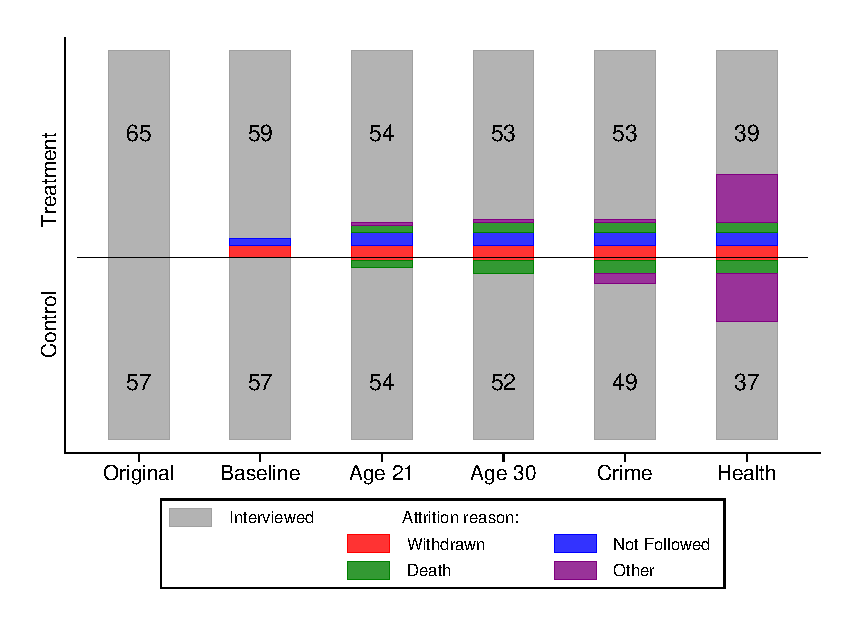
\includegraphics[width=.9\columnwidth]{output/abc_attrition.eps}
  \floatfoot{
\footnotesize
Note: This plot shows the number of participants in ABC for whom there exists data at the periods of data collection by experimental group. The subjects who withdrew from the study did so due to several reasons, such as adoption. Subjects were not followed if they were found to be biologically retarded after randomization. The numbers in the bars indicate the number of individuals who were interviewed during that phase of data collection. The original sample was measured after randomization but before the start of the program, the baseline sample was measured at the start of the program, and the health sample was collected at age 34.
}
\end{figure}
\end{comment}

\noindent Attrition was low in ABC. Information is available on 100 subjects in the age 30 follow-up, which we call the adult follow-up. In addition, 80 participants from the control group and 40 from the treatment group consented to the release of their criminal records. Further, 70 participants consented to the release of information regarding a full-range biomedical panel, 31 from the control group and 39 from the treatment group. \\

\noindent Attrition was also low for CARE subjects. Information is available on 58 subjects (more than 85\% of the initial sample) in the age-30 follow-up. Additionally, 40 participants (11 from the control group, 18 from the family education group, and 11 from the center-based preschool and family education group) released information on the full-range biomedical sweep. Administrative crime data are not available for CARE. We do not evaluate the second-phase of treatment in CARE because it was not randomized. Rather, those in the center-based preschool and family education group and the family education group were offered school-age treatment, and those in the control group were not.  \\ 

\noindent In the following set of tables (Table~\ref{tab:abc_baseline} through Table~\ref{tab:health_baseline}), we compare the observed, baseline characteristics between the first-phase control and treatment groups in ABC, which are the main groups we analyze, at different stages of the data collection follow-ups. For each observed characteristic, we present the bootstrapped $p$-value associated with the standard $t$-test. We also present the bootstrapped, step-down $p$-value on jointly testing the difference in observed characteristics across the two blocks of variables separated by the horizontal line \citep{Lehmann_Romano_2005_testing}.\\

\noindent First, we compare the first-phase treatment and control groups on baseline characteristics. 

\begin{table}[H]
\captionsetup{singlelinecheck=false,justification=centering}
\caption{First-phase Treatment vs. Control Groups \label{tab:baseline}}

  \begin{threeparttable}
  \begin{tabular}{cccccccc}
  \hline\hline

     &  & \scriptsize{Control} & \scriptsize{Treated} & \scriptsize{Control} & \scriptsize{Treated} & \mc{2}{c}{\scriptsize{$p$-value}} \\  

    \scriptsize{Variable} & \scriptsize{Age} & \scriptsize{Obs.} & \scriptsize{Obs.} & \scriptsize{Mean} & \scriptsize{Mean} & \scriptsize{Single $H_0$} & \scriptsize{Multiple $H_0$} \\ 
    \hline  

    \mc{1}{l}{\scriptsize{Male}} & \mc{1}{c}{\scriptsize{0}} & \mc{1}{c}{\scriptsize{57}} & \mc{1}{c}{\scriptsize{59}} & \mc{1}{c}{\scriptsize{0.438}} & \mc{1}{c}{\scriptsize{0.489}} & \mc{1}{c}{\scriptsize{(0.580)}} & \mc{1}{c}{\scriptsize{(0.700)}} \\  

    \mc{1}{l}{\scriptsize{Birth Weight}} & \mc{1}{c}{\scriptsize{0}} & \mc{1}{c}{\scriptsize{56}} & \mc{1}{c}{\scriptsize{58}} & \mc{1}{c}{\scriptsize{7.191}} & \mc{1}{c}{\scriptsize{6.829}} & \mc{1}{c}{\scriptsize{(0.130)}} & \mc{1}{c}{\scriptsize{(0.205)}} \\  

    \mc{1}{l}{\scriptsize{No. Siblings in Household}} & \mc{1}{c}{\scriptsize{0}} & \mc{1}{c}{\scriptsize{57}} & \mc{1}{c}{\scriptsize{59}} & \mc{1}{c}{\scriptsize{0.750}} & \mc{1}{c}{\scriptsize{0.516}} & \mc{1}{c}{\scriptsize{(0.245)}} & \mc{1}{c}{\scriptsize{(0.425)}} \\  

    \mc{1}{l}{\scriptsize{Birth Year}} & \mc{1}{c}{\scriptsize{0}} & \mc{1}{c}{\scriptsize{57}} & \mc{1}{c}{\scriptsize{59}} & \mc{1}{c}{\scriptsize{1974}} & \mc{1}{c}{\scriptsize{1974}} & \mc{1}{c}{\scriptsize{(0.785)}} & \mc{1}{c}{\scriptsize{(0.865)}} \\ 
    \hline  

    \mc{1}{l}{\scriptsize{Mother's Education}} & \mc{1}{c}{\scriptsize{0}} & \mc{1}{c}{\scriptsize{57}} & \mc{1}{c}{\scriptsize{59}} & \mc{1}{c}{\scriptsize{9.864}} & \mc{1}{c}{\scriptsize{10.505}} & \mc{1}{c}{\scriptsize{\textbf{(0.050)}}} & \mc{1}{c}{\scriptsize{\textbf{(0.090)}}} \\  

    \mc{1}{l}{\scriptsize{Mother's Age}} & \mc{1}{c}{\scriptsize{0}} & \mc{1}{c}{\scriptsize{57}} & \mc{1}{c}{\scriptsize{59}} & \mc{1}{c}{\scriptsize{20.103}} & \mc{1}{c}{\scriptsize{19.564}} & \mc{1}{c}{\scriptsize{(0.555)}} & \mc{1}{c}{\scriptsize{(0.665)}} \\  

    \mc{1}{l}{\scriptsize{Parental Income}} & \mc{1}{c}{\scriptsize{0}} & \mc{1}{c}{\scriptsize{57}} & \mc{1}{c}{\scriptsize{58}} & \mc{1}{c}{\scriptsize{6,211}} & \mc{1}{c}{\scriptsize{7,019}} & \mc{1}{c}{\scriptsize{(0.645)}} & \mc{1}{c}{\scriptsize{(0.720)}} \\  

    \mc{1}{l}{\scriptsize{Mother's IQ}} & \mc{1}{c}{\scriptsize{0}} & \mc{1}{c}{\scriptsize{57}} & \mc{1}{c}{\scriptsize{59}} & \mc{1}{c}{\scriptsize{83.419}} & \mc{1}{c}{\scriptsize{85.393}} & \mc{1}{c}{\scriptsize{(0.360)}} & \mc{1}{c}{\scriptsize{(0.510)}} \\  

    \mc{1}{l}{\scriptsize{Father at Home}} & \mc{1}{c}{\scriptsize{0}} & \mc{1}{c}{\scriptsize{57}} & \mc{1}{c}{\scriptsize{59}} & \mc{1}{c}{\scriptsize{0.346}} & \mc{1}{c}{\scriptsize{0.223}} & \mc{1}{c}{\scriptsize{(0.135)}} & \mc{1}{c}{\scriptsize{(0.270)}} \\  

  \hline\hline
  \end{tabular}
    \begin{tablenotes}
    \scriptsize
    \item 
    Note: This table shows the balance in observed characteristics between the treatment and control groups at baseline.
    For each characteristic, we present the $p$-value from a single hypothesis test.
    We also present the $p$-values from multiple testing, where we collectively test the
    baseline characteristics within the blocks separated by the horizontal line.
    Both $p$-values are two-sided and non-parametric. We construct them 
    based on 1,000 re-draws of the full sample. The estimates we display are the means of 
    the empirical bootstrap distribution. 
    
    \end{tablenotes}
  \end{threeparttable}

\end{table}

\noindent Second, we present the same exercise for each of the four cohorts ABC served.

\begin{table}[H]
\captionsetup{singlelinecheck=false,justification=centering}
\caption{First-phase Treatment vs. Control Groups, ABC Cohort 1 \label{tab:baseline_coh1}}

  \begin{threeparttable}
  \begin{tabular}{cccccccc}
  \toprule

     &  & \scriptsize{Control} & \scriptsize{Treated} & \scriptsize{Control} & \scriptsize{Treated} & \mc{2}{c}{\scriptsize{$p$-value}} \\  

    \scriptsize{Variable} & \scriptsize{Age} & \scriptsize{Obs.} & \scriptsize{Obs.} & \scriptsize{Mean} & \scriptsize{Mean} & \scriptsize{Single $H_0$} & \scriptsize{Multiple $H_0$} \\ 
    \midrule  

    \mc{1}{l}{\scriptsize{Male}} & \mc{1}{c}{\scriptsize{0}} & \mc{1}{c}{\scriptsize{14}} & \mc{1}{c}{\scriptsize{14}} & \mc{1}{c}{\scriptsize{0.348}} & \mc{1}{c}{\scriptsize{0.286}} & \mc{1}{c}{\scriptsize{(0.730)}} & \mc{1}{c}{\scriptsize{(0.738)}} \\  

    \mc{1}{l}{\scriptsize{Birth Weight}} & \mc{1}{c}{\scriptsize{0}} & \mc{1}{c}{\scriptsize{14}} & \mc{1}{c}{\scriptsize{13}} & \mc{1}{c}{\scriptsize{6.755}} & \mc{1}{c}{\scriptsize{6.491}} & \mc{1}{c}{\scriptsize{(0.550)}} & \mc{1}{c}{\scriptsize{(0.655)}} \\  

    \mc{1}{l}{\scriptsize{No. Siblings in Household}} & \mc{1}{c}{\scriptsize{0}} & \mc{1}{c}{\scriptsize{14}} & \mc{1}{c}{\scriptsize{14}} & \mc{1}{c}{\scriptsize{1.741}} & \mc{1}{c}{\scriptsize{0.606}} & \mc{1}{c}{\scriptsize{\textbf{(0.035)}}} & \mc{1}{c}{\scriptsize{\textbf{(0.085)}}} \\  

    \mc{1}{l}{\scriptsize{Birth Year}} & \mc{1}{c}{\scriptsize{0}} & \mc{1}{c}{\scriptsize{14}} & \mc{1}{c}{\scriptsize{14}} & \mc{1}{c}{\scriptsize{1972}} & \mc{1}{c}{\scriptsize{1972}} & \mc{1}{c}{\scriptsize{(0.240)}} & \mc{1}{c}{\scriptsize{(0.350)}} \\ 
    \midrule 

    \mc{1}{l}{\scriptsize{Mother's Education}} & \mc{1}{c}{\scriptsize{0}} & \mc{1}{c}{\scriptsize{14}} & \mc{1}{c}{\scriptsize{14}} & \mc{1}{c}{\scriptsize{9.885}} & \mc{1}{c}{\scriptsize{10.561}} & \mc{1}{c}{\scriptsize{(0.265)}} & \mc{1}{c}{\scriptsize{(0.480)}} \\  

    \mc{1}{l}{\scriptsize{Mother's Age}} & \mc{1}{c}{\scriptsize{0}} & \mc{1}{c}{\scriptsize{14}} & \mc{1}{c}{\scriptsize{14}} & \mc{1}{c}{\scriptsize{23.869}} & \mc{1}{c}{\scriptsize{19.552}} & \mc{1}{c}{\scriptsize{\textbf{(0.050)}}} & \mc{1}{c}{\scriptsize{(0.135)}} \\  

    \mc{1}{l}{\scriptsize{Mother Employed}} & \mc{1}{c}{\scriptsize{0}} & \mc{1}{c}{\scriptsize{14}} & \mc{1}{c}{\scriptsize{14}} & \mc{1}{c}{\scriptsize{0.152}} & \mc{1}{c}{\scriptsize{0.205}} & \mc{1}{c}{\scriptsize{(0.695)}} & \mc{1}{c}{\scriptsize{(0.895)}} \\  

    \mc{1}{l}{\scriptsize{Parental Income}} & \mc{1}{c}{\scriptsize{0}} & \mc{1}{c}{\scriptsize{14}} & \mc{1}{c}{\scriptsize{13}} & \mc{1}{c}{\scriptsize{7,164}} & \mc{1}{c}{\scriptsize{8,298}} & \mc{1}{c}{\scriptsize{(0.755)}} & \mc{1}{c}{\scriptsize{(0.910)}} \\  

    \mc{1}{l}{\scriptsize{Mother's IQ}} & \mc{1}{c}{\scriptsize{0}} & \mc{1}{c}{\scriptsize{14}} & \mc{1}{c}{\scriptsize{14}} & \mc{1}{c}{\scriptsize{76.042}} & \mc{1}{c}{\scriptsize{81.108}} & \mc{1}{c}{\scriptsize{(0.270)}} & \mc{1}{c}{\scriptsize{(0.485)}} \\  

    \mc{1}{l}{\scriptsize{Father at Home}} & \mc{1}{c}{\scriptsize{0}} & \mc{1}{c}{\scriptsize{14}} & \mc{1}{c}{\scriptsize{14}} & \mc{1}{c}{\scriptsize{0.559}} & \mc{1}{c}{\scriptsize{0.368}} & \mc{1}{c}{\scriptsize{(0.340)}} & \mc{1}{c}{\scriptsize{(0.493)}} \\  

  \bottomrule
  \end{tabular}
    \begin{tablenotes}
    \scriptsize
    \item 
    Note: This table shows the balance in observed characteristics between the treatment and control groups in ABC at baseline for cohort 1.
    For each characteristic, we present the $p$-value from a single hypothesis test.
    We also present the $p$-values from multiple hypothesis testing, where we collectively test the
    baseline characteristics within the blocks separated by the horizontal line.
    Both $p$-values are two-sided and non-parametric. We construct them 
    based on 200 re-draws of the full sample.
    
    \end{tablenotes}
  \end{threeparttable}

\end{table}

\begin{table}[H]
\captionsetup{singlelinecheck=false,justification=centering}
\caption{First-phase Treatment vs. Control Groups, ABC Cohort 2 \label{tab:baseline_coh2}}

  \begin{threeparttable}
  \begin{tabular}{cccccccc}
  \toprule

     &  & \scriptsize{Control} & \scriptsize{Treated} & \scriptsize{Control} & \scriptsize{Treated} & \mc{2}{c}{\scriptsize{$p$-value}} \\  

    \scriptsize{Variable} & \scriptsize{Age} & \scriptsize{Obs.} & \scriptsize{Obs.} & \scriptsize{Mean} & \scriptsize{Mean} & \scriptsize{Single $H_0$} & \scriptsize{Multiple $H_0$} \\ 
    \midrule

    \mc{1}{l}{\scriptsize{Male}} & \mc{1}{c}{\scriptsize{0}} & \mc{1}{c}{\scriptsize{13}} & \mc{1}{c}{\scriptsize{16}} & \mc{1}{c}{\scriptsize{0.457}} & \mc{1}{c}{\scriptsize{0.503}} & \mc{1}{c}{\scriptsize{(0.805)}} & \mc{1}{c}{\scriptsize{(0.875)}} \\  

    \mc{1}{l}{\scriptsize{Birth Weight}} & \mc{1}{c}{\scriptsize{0}} & \mc{1}{c}{\scriptsize{13}} & \mc{1}{c}{\scriptsize{16}} & \mc{1}{c}{\scriptsize{7.256}} & \mc{1}{c}{\scriptsize{6.534}} & \mc{1}{c}{\scriptsize{(0.160)}} & \mc{1}{c}{\scriptsize{(0.270)}} \\  

    \mc{1}{l}{\scriptsize{No. Siblings in Household}} & \mc{1}{c}{\scriptsize{0}} & \mc{1}{c}{\scriptsize{13}} & \mc{1}{c}{\scriptsize{16}} & \mc{1}{c}{\scriptsize{0.388}} & \mc{1}{c}{\scriptsize{0.316}} & \mc{1}{c}{\scriptsize{(0.755)}} & \mc{1}{c}{\scriptsize{(0.835)}} \\  

    \mc{1}{l}{\scriptsize{Birth Year}} & \mc{1}{c}{\scriptsize{0}} & \mc{1}{c}{\scriptsize{13}} & \mc{1}{c}{\scriptsize{16}} & \mc{1}{c}{\scriptsize{1973}} & \mc{1}{c}{\scriptsize{1973}} & \mc{1}{c}{\scriptsize{(0.850)}} & \mc{1}{c}{\scriptsize{(0.925)}} \\ 
    \midrule  

    \mc{1}{l}{\scriptsize{Mother's Education}} & \mc{1}{c}{\scriptsize{0}} & \mc{1}{c}{\scriptsize{13}} & \mc{1}{c}{\scriptsize{16}} & \mc{1}{c}{\scriptsize{10.225}} & \mc{1}{c}{\scriptsize{10.307}} & \mc{1}{c}{\scriptsize{(0.885)}} & \mc{1}{c}{\scriptsize{(0.940)}} \\  

    \mc{1}{l}{\scriptsize{Mother's Age}} & \mc{1}{c}{\scriptsize{0}} & \mc{1}{c}{\scriptsize{13}} & \mc{1}{c}{\scriptsize{16}} & \mc{1}{c}{\scriptsize{18.446}} & \mc{1}{c}{\scriptsize{17.637}} & \mc{1}{c}{\scriptsize{(0.380)}} & \mc{1}{c}{\scriptsize{(0.630)}} \\  

    \mc{1}{l}{\scriptsize{Mother Employed}} & \mc{1}{c}{\scriptsize{0}} & \mc{1}{c}{\scriptsize{13}} & \mc{1}{c}{\scriptsize{16}} & \mc{1}{c}{\scriptsize{0.307}} & \mc{1}{c}{\scriptsize{0.248}} & \mc{1}{c}{\scriptsize{(0.690)}} & \mc{1}{c}{\scriptsize{(0.850)}} \\  

    \mc{1}{l}{\scriptsize{Parental Income}} & \mc{1}{c}{\scriptsize{0}} & \mc{1}{c}{\scriptsize{13}} & \mc{1}{c}{\scriptsize{16}} & \mc{1}{c}{\scriptsize{5,398}} & \mc{1}{c}{\scriptsize{4,427}} & \mc{1}{c}{\scriptsize{(0.790)}} & \mc{1}{c}{\scriptsize{(0.880)}} \\  

    \mc{1}{l}{\scriptsize{Mother's IQ}} & \mc{1}{c}{\scriptsize{0}} & \mc{1}{c}{\scriptsize{13}} & \mc{1}{c}{\scriptsize{16}} & \mc{1}{c}{\scriptsize{86.873}} & \mc{1}{c}{\scriptsize{85.597}} & \mc{1}{c}{\scriptsize{(0.730)}} & \mc{1}{c}{\scriptsize{(0.855)}} \\  

    \mc{1}{l}{\scriptsize{Father at Home}} & \mc{1}{c}{\scriptsize{0}} & \mc{1}{c}{\scriptsize{13}} & \mc{1}{c}{\scriptsize{16}} & \mc{1}{c}{\scriptsize{0.220}} & \mc{1}{c}{\scriptsize{0.183}} & \mc{1}{c}{\scriptsize{(0.790)}} & \mc{1}{c}{\scriptsize{(0.895)}} \\  

  \bottomrule
  \end{tabular}
    \begin{tablenotes}
    \scriptsize
    \item 
    Note: This table shows the balance in observed characteristics between the treatment and control groups in ABC at baseline for cohort 2.
    For each characteristic, we present the $p$-value from a single hypothesis test.
    We also present the $p$-values from multiple hypothesis testing, where we collectively test the
    baseline characteristics within the blocks separated by the horizontal line.
    Both $p$-values are two-sided and non-parametric. We construct them 
    based on 200 re-draws of the full sample.
    
    \end{tablenotes}
  \end{threeparttable}

\end{table}

\begin{table}[H]
\captionsetup{singlelinecheck=false,justification=centering}
\caption{First-phase Treatment vs. Control Groups, ABC Cohort 3 \label{tab:baseline_coh3}}

  \begin{threeparttable}
  \begin{tabular}{cccccccc}
  \hline\hline

     &  & \scriptsize{Control} & \scriptsize{Treated} & \scriptsize{Control} & \scriptsize{Treated} & \mc{2}{c}{\scriptsize{$p$-value}} \\  

    \scriptsize{Variable} & \scriptsize{Age} & \scriptsize{Obs.} & \scriptsize{Obs.} & \scriptsize{Mean} & \scriptsize{Mean} & \scriptsize{Single $H_0$} & \scriptsize{Multiple $H_0$} \\ 
    \hline  

    \mc{1}{l}{\scriptsize{Male}} & \mc{1}{c}{\scriptsize{0}} & \mc{1}{c}{\scriptsize{14}} & \mc{1}{c}{\scriptsize{15}} & \mc{1}{c}{\scriptsize{0.376}} & \mc{1}{c}{\scriptsize{0.596}} & \mc{1}{c}{\scriptsize{(0.265)}} & \mc{1}{c}{\scriptsize{(0.320)}} \\  

    \mc{1}{l}{\scriptsize{Birth Weight}} & \mc{1}{c}{\scriptsize{0}} & \mc{1}{c}{\scriptsize{14}} & \mc{1}{c}{\scriptsize{15}} & \mc{1}{c}{\scriptsize{7.424}} & \mc{1}{c}{\scriptsize{7.138}} & \mc{1}{c}{\scriptsize{(0.470)}} & \mc{1}{c}{\scriptsize{(0.730)}} \\  

    \mc{1}{l}{\scriptsize{No. Siblings in Household}} & \mc{1}{c}{\scriptsize{0}} & \mc{1}{c}{\scriptsize{14}} & \mc{1}{c}{\scriptsize{15}} & \mc{1}{c}{\scriptsize{0.423}} & \mc{1}{c}{\scriptsize{0.203}} & \mc{1}{c}{\scriptsize{(0.385)}} & \mc{1}{c}{\scriptsize{(0.645)}} \\  

    \mc{1}{l}{\scriptsize{Birth Year}} & \mc{1}{c}{\scriptsize{0}} & \mc{1}{c}{\scriptsize{14}} & \mc{1}{c}{\scriptsize{15}} & \mc{1}{c}{\scriptsize{1975}} & \mc{1}{c}{\scriptsize{1975}} & \mc{1}{c}{\scriptsize{(0.510)}} & \mc{1}{c}{\scriptsize{(0.520)}} \\ 
    \hline  

    \mc{1}{l}{\scriptsize{Mother's Education}} & \mc{1}{c}{\scriptsize{0}} & \mc{1}{c}{\scriptsize{14}} & \mc{1}{c}{\scriptsize{15}} & \mc{1}{c}{\scriptsize{10.133}} & \mc{1}{c}{\scriptsize{10.704}} & \mc{1}{c}{\scriptsize{(0.405)}} & \mc{1}{c}{\scriptsize{(0.595)}} \\  

    \mc{1}{l}{\scriptsize{Mother's Age}} & \mc{1}{c}{\scriptsize{0}} & \mc{1}{c}{\scriptsize{14}} & \mc{1}{c}{\scriptsize{15}} & \mc{1}{c}{\scriptsize{18.602}} & \mc{1}{c}{\scriptsize{19.558}} & \mc{1}{c}{\scriptsize{(0.355)}} & \mc{1}{c}{\scriptsize{(0.570)}} \\  

    \mc{1}{l}{\scriptsize{Mother Employed}} & \mc{1}{c}{\scriptsize{0}} & \mc{1}{c}{\scriptsize{14}} & \mc{1}{c}{\scriptsize{15}} & \mc{1}{c}{\scriptsize{0.162}} & \mc{1}{c}{\scriptsize{0.467}} & \mc{1}{c}{\scriptsize{\textbf{(0.070)}}} & \mc{1}{c}{\scriptsize{(0.155)}} \\  

    \mc{1}{l}{\scriptsize{Parental Income}} & \mc{1}{c}{\scriptsize{0}} & \mc{1}{c}{\scriptsize{14}} & \mc{1}{c}{\scriptsize{15}} & \mc{1}{c}{\scriptsize{7,034}} & \mc{1}{c}{\scriptsize{4,981}} & \mc{1}{c}{\scriptsize{(0.430)}} & \mc{1}{c}{\scriptsize{(0.675)}} \\  

    \mc{1}{l}{\scriptsize{Mother's IQ}} & \mc{1}{c}{\scriptsize{0}} & \mc{1}{c}{\scriptsize{14}} & \mc{1}{c}{\scriptsize{15}} & \mc{1}{c}{\scriptsize{85.590}} & \mc{1}{c}{\scriptsize{88.715}} & \mc{1}{c}{\scriptsize{(0.435)}} & \mc{1}{c}{\scriptsize{(0.610)}} \\  

    \mc{1}{l}{\scriptsize{Father at Home}} & \mc{1}{c}{\scriptsize{0}} & \mc{1}{c}{\scriptsize{14}} & \mc{1}{c}{\scriptsize{15}} & \mc{1}{c}{\scriptsize{0.424}} & \mc{1}{c}{\scriptsize{0.209}} & \mc{1}{c}{\scriptsize{(0.265)}} & \mc{1}{c}{\scriptsize{(0.425)}} \\  

  \hline\hline
  \end{tabular}
    \begin{tablenotes}
    \scriptsize
    \item 
    Note: This table shows the balance in observed characteristics between the treatment and control groups in ABC at baseline for cohort 3.
    For each characteristic, we present the $p$-value from a single hypothesis test.
    We also present the $p$-values from multiple testing, where we collectively test the
    baseline characteristics within the blocks separated by the horizontal line.
    Both $p$-values are two-sided and non-parametric. We construct them 
    based on 200 re-draws of the full sample. The estimates we display are the means of 
    the empirical bootstrap distribution. 
    
    \end{tablenotes}
  \end{threeparttable}

\end{table}

\begin{table}[H]
\captionsetup{singlelinecheck=false,justification=centering}
\caption{First-phase Treatment vs. Control Groups, ABC Cohort 4 \label{tab:baseline_coh4}}

  \begin{threeparttable}
  \begin{tabular}{cccccccc}
  \toprule

     &  & \scriptsize{Control} & \scriptsize{Treated} & \scriptsize{Control} & \scriptsize{Treated} & \mc{2}{c}{\scriptsize{$p$-value}} \\  

    \scriptsize{Variable} & \scriptsize{Age} & \scriptsize{Obs.} & \scriptsize{Obs.} & \scriptsize{Mean} & \scriptsize{Mean} & \scriptsize{Single $H_0$} & \scriptsize{Multiple $H_0$} \\ 
    \midrule

    \mc{1}{l}{\scriptsize{Male}} & \mc{1}{c}{\scriptsize{0}} & \mc{1}{c}{\scriptsize{15}} & \mc{1}{c}{\scriptsize{14}} & \mc{1}{c}{\scriptsize{0.599}} & \mc{1}{c}{\scriptsize{0.567}} & \mc{1}{c}{\scriptsize{(0.870)}} & \mc{1}{c}{\scriptsize{(0.905)}} \\  

    \mc{1}{l}{\scriptsize{Birth Weight}} & \mc{1}{c}{\scriptsize{0}} & \mc{1}{c}{\scriptsize{15}} & \mc{1}{c}{\scriptsize{14}} & \mc{1}{c}{\scriptsize{7.321}} & \mc{1}{c}{\scriptsize{7.150}} & \mc{1}{c}{\scriptsize{(0.725)}} & \mc{1}{c}{\scriptsize{(0.840)}} \\  

    \mc{1}{l}{\scriptsize{No. Siblings in Household}} & \mc{1}{c}{\scriptsize{0}} & \mc{1}{c}{\scriptsize{15}} & \mc{1}{c}{\scriptsize{14}} & \mc{1}{c}{\scriptsize{0.490}} & \mc{1}{c}{\scriptsize{0.977}} & \mc{1}{c}{\scriptsize{(0.220)}} & \mc{1}{c}{\scriptsize{(0.380)}} \\  

    \mc{1}{l}{\scriptsize{Birth Year}} & \mc{1}{c}{\scriptsize{0}} & \mc{1}{c}{\scriptsize{15}} & \mc{1}{c}{\scriptsize{14}} & \mc{1}{c}{\scriptsize{1977}} & \mc{1}{c}{\scriptsize{1977}} & \mc{1}{c}{\scriptsize{(0.615)}} & \mc{1}{c}{\scriptsize{(0.728)}} \\ 
    \midrule

    \mc{1}{l}{\scriptsize{Mother's Education}} & \mc{1}{c}{\scriptsize{0}} & \mc{1}{c}{\scriptsize{15}} & \mc{1}{c}{\scriptsize{14}} & \mc{1}{c}{\scriptsize{9.530}} & \mc{1}{c}{\scriptsize{10.424}} & \mc{1}{c}{\scriptsize{(0.240)}} & \mc{1}{c}{\scriptsize{(0.410)}} \\  

    \mc{1}{l}{\scriptsize{Mother's Age}} & \mc{1}{c}{\scriptsize{0}} & \mc{1}{c}{\scriptsize{15}} & \mc{1}{c}{\scriptsize{14}} & \mc{1}{c}{\scriptsize{19.941}} & \mc{1}{c}{\scriptsize{21.712}} & \mc{1}{c}{\scriptsize{(0.320)}} & \mc{1}{c}{\scriptsize{(0.570)}} \\  

    \mc{1}{l}{\scriptsize{Mother Employed}} & \mc{1}{c}{\scriptsize{0}} & \mc{1}{c}{\scriptsize{15}} & \mc{1}{c}{\scriptsize{14}} & \mc{1}{c}{\scriptsize{0.260}} & \mc{1}{c}{\scriptsize{0.347}} & \mc{1}{c}{\scriptsize{(0.650)}} & \mc{1}{c}{\scriptsize{(0.840)}} \\  

    \mc{1}{l}{\scriptsize{Parental Income}} & \mc{1}{c}{\scriptsize{0}} & \mc{1}{c}{\scriptsize{15}} & \mc{1}{c}{\scriptsize{14}} & \mc{1}{c}{\scriptsize{5,827}} & \mc{1}{c}{\scriptsize{10,781}} & \mc{1}{c}{\scriptsize{\textbf{(0.065)}}} & \mc{1}{c}{\scriptsize{(0.135)}} \\  

    \mc{1}{l}{\scriptsize{Mother's IQ}} & \mc{1}{c}{\scriptsize{0}} & \mc{1}{c}{\scriptsize{15}} & \mc{1}{c}{\scriptsize{14}} & \mc{1}{c}{\scriptsize{85.561}} & \mc{1}{c}{\scriptsize{86.004}} & \mc{1}{c}{\scriptsize{(0.920)}} & \mc{1}{c}{\scriptsize{(0.960)}} \\  

    \mc{1}{l}{\scriptsize{Father at Home}} & \mc{1}{c}{\scriptsize{0}} & \mc{1}{c}{\scriptsize{15}} & \mc{1}{c}{\scriptsize{14}} & \mc{1}{c}{\scriptsize{0.208}} & \mc{1}{c}{\scriptsize{0.138}} & \mc{1}{c}{\scriptsize{(0.570)}} & \mc{1}{c}{\scriptsize{(0.777)}} \\  

  \bottomrule
  \end{tabular}
    \begin{tablenotes}
    \scriptsize
    \item 
    Note: This table shows the balance in observed characteristics between the treatment and control groups in ABC at baseline for cohort 4.
    For each characteristic, we present the $p$-value from a single hypothesis test.
    We also present the $p$-values from multiple hypothesis testing, where we collectively test the
    baseline characteristics within the blocks separated by the horizontal line.
    Both $p$-values are two-sided and non-parametric. We construct them 
    based on 200 re-draws of the full sample. The estimates we display are the means of 
    the empirical bootstrap distribution. 
    
    \end{tablenotes}
  \end{threeparttable}

\end{table}

\noindent Third, we compare the second-phase treatment and control groups on baseline characteristics. 

\begin{table}[H]
\captionsetup{singlelinecheck=false,justification=centering}
\caption{Second-phase Treatment vs. Control Groups \label{tab:baseline_sa}}

  \begin{threeparttable}
  \begin{tabular}{cccccccc}
  \hline\hline

     &  & \scriptsize{Control} & \scriptsize{Treatment} & \scriptsize{Control} & \scriptsize{Treated} & \mc{2}{c}{\scriptsize{$p$-value}} \\  

    \scriptsize{Variable} & \scriptsize{Age} & \scriptsize{Obs.} & \scriptsize{Obs.} & \scriptsize{Mean} & \scriptsize{Mean} & \scriptsize{Single $H_0$} & \scriptsize{Multiple $H_0$} \\ 
    \hline  

    \mc{1}{l}{\scriptsize{Male}} & \mc{1}{c}{\scriptsize{0}} & \mc{1}{c}{\scriptsize{47}} & \mc{1}{c}{\scriptsize{48}} & \mc{1}{c}{\scriptsize{0.551}} & \mc{1}{c}{\scriptsize{0.460}} & \mc{1}{c}{\scriptsize{(0.420)}} & \mc{1}{c}{\scriptsize{(0.552)}} \\  

    \mc{1}{l}{\scriptsize{Birth Weight}} & \mc{1}{c}{\scriptsize{0}} & \mc{1}{c}{\scriptsize{47}} & \mc{1}{c}{\scriptsize{48}} & \mc{1}{c}{\scriptsize{7.084}} & \mc{1}{c}{\scriptsize{6.929}} & \mc{1}{c}{\scriptsize{(0.610)}} & \mc{1}{c}{\scriptsize{(0.700)}} \\  

    \mc{1}{l}{\scriptsize{No. Siblings in Household}} & \mc{1}{c}{\scriptsize{0}} & \mc{1}{c}{\scriptsize{47}} & \mc{1}{c}{\scriptsize{48}} & \mc{1}{c}{\scriptsize{0.748}} & \mc{1}{c}{\scriptsize{0.504}} & \mc{1}{c}{\scriptsize{(0.285)}} & \mc{1}{c}{\scriptsize{(0.445)}} \\  

    \mc{1}{l}{\scriptsize{Birth Year}} & \mc{1}{c}{\scriptsize{0}} & \mc{1}{c}{\scriptsize{47}} & \mc{1}{c}{\scriptsize{48}} & \mc{1}{c}{\scriptsize{1974}} & \mc{1}{c}{\scriptsize{1974}} & \mc{1}{c}{\scriptsize{(0.835)}} & \mc{1}{c}{\scriptsize{(0.915)}} \\ 
    \hline  

    \mc{1}{l}{\scriptsize{Mother's Education}} & \mc{1}{c}{\scriptsize{0}} & \mc{1}{c}{\scriptsize{47}} & \mc{1}{c}{\scriptsize{48}} & \mc{1}{c}{\scriptsize{10.150}} & \mc{1}{c}{\scriptsize{10.388}} & \mc{1}{c}{\scriptsize{(0.480)}} & \mc{1}{c}{\scriptsize{(0.685)}} \\  

    \mc{1}{l}{\scriptsize{Mother's Age}} & \mc{1}{c}{\scriptsize{0}} & \mc{1}{c}{\scriptsize{47}} & \mc{1}{c}{\scriptsize{48}} & \mc{1}{c}{\scriptsize{21.122}} & \mc{1}{c}{\scriptsize{18.884}} & \mc{1}{c}{\scriptsize{\textbf{(0.035)}}} & \mc{1}{c}{\scriptsize{\textbf{(0.065)}}} \\  

    \mc{1}{l}{\scriptsize{Parental Income}} & \mc{1}{c}{\scriptsize{0}} & \mc{1}{c}{\scriptsize{47}} & \mc{1}{c}{\scriptsize{48}} & \mc{1}{c}{\scriptsize{7,589}} & \mc{1}{c}{\scriptsize{6,714}} & \mc{1}{c}{\scriptsize{(0.625)}} & \mc{1}{c}{\scriptsize{(0.795)}} \\  

    \mc{1}{l}{\scriptsize{Mother's IQ}} & \mc{1}{c}{\scriptsize{0}} & \mc{1}{c}{\scriptsize{47}} & \mc{1}{c}{\scriptsize{48}} & \mc{1}{c}{\scriptsize{83.000}} & \mc{1}{c}{\scriptsize{85.831}} & \mc{1}{c}{\scriptsize{(0.185)}} & \mc{1}{c}{\scriptsize{(0.350)}} \\  

    \mc{1}{l}{\scriptsize{Father at Home}} & \mc{1}{c}{\scriptsize{0}} & \mc{1}{c}{\scriptsize{47}} & \mc{1}{c}{\scriptsize{48}} & \mc{1}{c}{\scriptsize{0.279}} & \mc{1}{c}{\scriptsize{0.287}} & \mc{1}{c}{\scriptsize{(0.920)}} & \mc{1}{c}{\scriptsize{(0.965)}} \\  

  \hline\hline
  \end{tabular}
    \begin{tablenotes}
    \scriptsize
    \item 
    Note: This table shows the balance in observed characteristics between the school-age treatment and control groups at baseline.
    For each characteristic, we present the $p$-value from a single hypothesis test.
    We also present the $p$-values from multiple testing, where we collectively test the
    baseline characteristics within the blocks separated by the horizontal line.
    Both $p$-values are two-sided and non-parametric. We construct them 
    based on 200 re-draws of the full sample. The estimates we display are the means of 
    the empirical bootstrap distribution. 
    
    \end{tablenotes}
  \end{threeparttable}

\end{table}

\noindent Fourth, we compare the observed, baseline characteristics of compliant and non-compliant subjects in the first-phase treatment assignment.

\begin{table}[H]
\captionsetup{singlelinecheck=false,justification=centering}
\caption{Observed vs. Attritted Children, ABC \label{tab:attrition_baseline}}

  \begin{threeparttable}
  \begin{tabular}{cccccccc}
  \toprule

     &  &  &  & \scriptsize{Observed} & \scriptsize{Attritted} & \mc{2}{c}{\scriptsize{$p$-value}} \\  

    \scriptsize{Variable} & \scriptsize{Age} & \scriptsize{Obs.} & \scriptsize{Att.} & \scriptsize{Mean} & \scriptsize{Mean} & \scriptsize{Single $H_0$} & \scriptsize{Multiple $H_0$} \\ 
    \midrule

    \mc{1}{l}{\scriptsize{Male}} & \mc{1}{c}{\scriptsize{0}} & \mc{1}{c}{\scriptsize{103}} & \mc{1}{c}{\scriptsize{13}} & \mc{1}{c}{\scriptsize{0.488}} & \mc{1}{c}{\scriptsize{0.248}} & \mc{1}{c}{\scriptsize{\textbf{(0.085)}}} & \mc{1}{c}{\scriptsize{(0.140)}} \\  

    \mc{1}{l}{\scriptsize{Birth Weight}} & \mc{1}{c}{\scriptsize{0}} & \mc{1}{c}{\scriptsize{103}} & \mc{1}{c}{\scriptsize{11}} & \mc{1}{c}{\scriptsize{7.014}} & \mc{1}{c}{\scriptsize{6.948}} & \mc{1}{c}{\scriptsize{(0.825)}} & \mc{1}{c}{\scriptsize{(0.875)}} \\  

    \mc{1}{l}{\scriptsize{No. Siblings in Household}} & \mc{1}{c}{\scriptsize{0}} & \mc{1}{c}{\scriptsize{103}} & \mc{1}{c}{\scriptsize{13}} & \mc{1}{c}{\scriptsize{0.609}} & \mc{1}{c}{\scriptsize{0.829}} & \mc{1}{c}{\scriptsize{(0.600)}} & \mc{1}{c}{\scriptsize{(0.705)}} \\  

    \mc{1}{l}{\scriptsize{Birth Year}} & \mc{1}{c}{\scriptsize{0}} & \mc{1}{c}{\scriptsize{103}} & \mc{1}{c}{\scriptsize{13}} & \mc{1}{c}{\scriptsize{1974}} & \mc{1}{c}{\scriptsize{1973}} & \mc{1}{c}{\scriptsize{\textbf{(0.045)}}} & \mc{1}{c}{\scriptsize{\textbf{(0.095)}}} \\ 
    \midrule

    \mc{1}{l}{\scriptsize{Mother's Education}} & \mc{1}{c}{\scriptsize{0}} & \mc{1}{c}{\scriptsize{103}} & \mc{1}{c}{\scriptsize{13}} & \mc{1}{c}{\scriptsize{10.302}} & \mc{1}{c}{\scriptsize{9.192}} & \mc{1}{c}{\scriptsize{\textbf{(0.100)}}} & \mc{1}{c}{\scriptsize{(0.165)}} \\  

    \mc{1}{l}{\scriptsize{Mother's Age}} & \mc{1}{c}{\scriptsize{0}} & \mc{1}{c}{\scriptsize{103}} & \mc{1}{c}{\scriptsize{13}} & \mc{1}{c}{\scriptsize{20.016}} & \mc{1}{c}{\scriptsize{18.178}} & \mc{1}{c}{\scriptsize{\textbf{(0.080)}}} & \mc{1}{c}{\scriptsize{(0.160)}} \\  

    \mc{1}{l}{\scriptsize{Mother Employed}} & \mc{1}{c}{\scriptsize{0}} & \mc{1}{c}{\scriptsize{103}} & \mc{1}{c}{\scriptsize{13}} & \mc{1}{c}{\scriptsize{0.268}} & \mc{1}{c}{\scriptsize{0.255}} & \mc{1}{c}{\scriptsize{(0.925)}} & \mc{1}{c}{\scriptsize{(0.955)}} \\  

    \mc{1}{l}{\scriptsize{Parental Income}} & \mc{1}{c}{\scriptsize{0}} & \mc{1}{c}{\scriptsize{103}} & \mc{1}{c}{\scriptsize{12}} & \mc{1}{c}{\scriptsize{6,622}} & \mc{1}{c}{\scriptsize{6,442}} & \mc{1}{c}{\scriptsize{(0.950)}} & \mc{1}{c}{\scriptsize{(0.960)}} \\  

    \mc{1}{l}{\scriptsize{Mother's IQ}} & \mc{1}{c}{\scriptsize{0}} & \mc{1}{c}{\scriptsize{103}} & \mc{1}{c}{\scriptsize{13}} & \mc{1}{c}{\scriptsize{85.050}} & \mc{1}{c}{\scriptsize{78.834}} & \mc{1}{c}{\scriptsize{\textbf{(0.070)}}} & \mc{1}{c}{\scriptsize{(0.135)}} \\  

    \mc{1}{l}{\scriptsize{Father at Home}} & \mc{1}{c}{\scriptsize{0}} & \mc{1}{c}{\scriptsize{103}} & \mc{1}{c}{\scriptsize{13}} & \mc{1}{c}{\scriptsize{0.278}} & \mc{1}{c}{\scriptsize{0.329}} & \mc{1}{c}{\scriptsize{(0.735)}} & \mc{1}{c}{\scriptsize{(0.835)}} \\  

  \bottomrule
  \end{tabular}
    \begin{tablenotes}
    \scriptsize
    \item 
    Note: This table shows the balance in observed characteristics between ABC subjects who were followed up to at least age 21 and ABC subjects who attrited before age 21.
    For each characteristic, we present the $p$-value from a single hypothesis test.
    We also present the $p$-values from multiple hypothesis testing, where we collectively test the
    baseline characteristics within the blocks separated by the horizontal line.
    Both $p$-values are two-sided and non-parametric. We construct them 
    based on 200 re-draws of the full sample. The estimates we display are the means of 
    the empirical bootstrap distribution. 
    
    \end{tablenotes}
  \end{threeparttable}

\end{table}

\noindent Fifth, we compare the observed, baseline characteristics between the subjects in the treatment and the control groups, excluding the subjects who did not comply to treatment.

\begin{table}[H]
\captionsetup{singlelinecheck=false,justification=centering}
\caption{First-stage Treatment vs. Control Groups, Dropping Attrited Children \label{tab:postattrition_baseline}}

  \begin{threeparttable}
  \begin{tabular}{cccccccc}
  \hline\hline

     &  & \scriptsize{Control} & \scriptsize{Treatment} & \scriptsize{Control} & \scriptsize{Treatment} & \mc{2}{c}{\scriptsize{$p$-value}} \\  

    \scriptsize{Variable} & \scriptsize{Age} & \scriptsize{Obs.} & \scriptsize{Obs.} & \scriptsize{Mean} & \scriptsize{Mean} & \scriptsize{Single $H_0$} & \scriptsize{Multiple $H_0$} \\ 
    \hline  

    \mc{1}{l}{\scriptsize{Male}} & \mc{1}{c}{\scriptsize{0}} & \mc{1}{c}{\scriptsize{51}} & \mc{1}{c}{\scriptsize{52}} & \mc{1}{c}{\scriptsize{0.452}} & \mc{1}{c}{\scriptsize{0.524}} & \mc{1}{c}{\scriptsize{(0.430)}} & \mc{1}{c}{\scriptsize{(0.600)}} \\  

    \mc{1}{l}{\scriptsize{Birth Weight}} & \mc{1}{c}{\scriptsize{0}} & \mc{1}{c}{\scriptsize{51}} & \mc{1}{c}{\scriptsize{52}} & \mc{1}{c}{\scriptsize{7.210}} & \mc{1}{c}{\scriptsize{6.822}} & \mc{1}{c}{\scriptsize{(0.115)}} & \mc{1}{c}{\scriptsize{(0.220)}} \\  

    \mc{1}{l}{\scriptsize{No. Siblings in Household}} & \mc{1}{c}{\scriptsize{0}} & \mc{1}{c}{\scriptsize{51}} & \mc{1}{c}{\scriptsize{52}} & \mc{1}{c}{\scriptsize{0.767}} & \mc{1}{c}{\scriptsize{0.455}} & \mc{1}{c}{\scriptsize{(0.150)}} & \mc{1}{c}{\scriptsize{(0.230)}} \\  

    \mc{1}{l}{\scriptsize{Birth Year}} & \mc{1}{c}{\scriptsize{0}} & \mc{1}{c}{\scriptsize{51}} & \mc{1}{c}{\scriptsize{52}} & \mc{1}{c}{\scriptsize{1974}} & \mc{1}{c}{\scriptsize{1974}} & \mc{1}{c}{\scriptsize{(0.635)}} & \mc{1}{c}{\scriptsize{(0.785)}} \\ 
    \hline  

    \mc{1}{l}{\scriptsize{Mother's Education}} & \mc{1}{c}{\scriptsize{0}} & \mc{1}{c}{\scriptsize{51}} & \mc{1}{c}{\scriptsize{52}} & \mc{1}{c}{\scriptsize{10.000}} & \mc{1}{c}{\scriptsize{10.598}} & \mc{1}{c}{\scriptsize{\textbf{(0.085)}}} & \mc{1}{c}{\scriptsize{(0.160)}} \\  

    \mc{1}{l}{\scriptsize{Mother's Age}} & \mc{1}{c}{\scriptsize{0}} & \mc{1}{c}{\scriptsize{51}} & \mc{1}{c}{\scriptsize{52}} & \mc{1}{c}{\scriptsize{20.412}} & \mc{1}{c}{\scriptsize{19.635}} & \mc{1}{c}{\scriptsize{(0.405)}} & \mc{1}{c}{\scriptsize{(0.580)}} \\  

    \mc{1}{l}{\scriptsize{Parental Income}} & \mc{1}{c}{\scriptsize{0}} & \mc{1}{c}{\scriptsize{51}} & \mc{1}{c}{\scriptsize{52}} & \mc{1}{c}{\scriptsize{6,409}} & \mc{1}{c}{\scriptsize{6,846}} & \mc{1}{c}{\scriptsize{(0.765)}} & \mc{1}{c}{\scriptsize{(0.835)}} \\  

    \mc{1}{l}{\scriptsize{Mother's IQ}} & \mc{1}{c}{\scriptsize{0}} & \mc{1}{c}{\scriptsize{51}} & \mc{1}{c}{\scriptsize{52}} & \mc{1}{c}{\scriptsize{84.472}} & \mc{1}{c}{\scriptsize{85.635}} & \mc{1}{c}{\scriptsize{(0.560)}} & \mc{1}{c}{\scriptsize{(0.715)}} \\  

    \mc{1}{l}{\scriptsize{Father at Home}} & \mc{1}{c}{\scriptsize{0}} & \mc{1}{c}{\scriptsize{51}} & \mc{1}{c}{\scriptsize{52}} & \mc{1}{c}{\scriptsize{0.349}} & \mc{1}{c}{\scriptsize{0.208}} & \mc{1}{c}{\scriptsize{(0.115)}} & \mc{1}{c}{\scriptsize{(0.225)}} \\  

  \hline\hline
  \end{tabular}
    \begin{tablenotes}
    \scriptsize
    \item 
    Note: This table shows the balance in observed characteristics between the treatment and control groups of subjects who were followed up to at least age 21.
    For each characteristic, we present the $p$-value from a single hypothesis test.
    We also present the $p$-values from multiple testing, where we collectively test the
    baseline characteristics within the blocks separated by the horizontal line.
    Both $p$-values are two-sided and non-parametric. We construct them 
    based on 1,000 re-draws of the full sample. The estimates we display are the means of 
    the empirical bootstrap distribution. 
    
    \end{tablenotes}
  \end{threeparttable}

\end{table}

% AZ: commenting out until we get the CORRECT numbers
\begin{comment}
\noindent Sixth, we compare the observed, baseline characteristics between the subjects in the first-phase treatment, restricting the sample to the subjects who consented to release their age-34 criminal records.

\begin{table}[H]
\captionsetup{singlelinecheck=false,justification=centering}
\caption{First-phase Treatment vs. Control Groups, Subjects who Released Criminal Records  \label{tab:crime_baseline}}

  \begin{threeparttable}
  \begin{tabular}{cccccccc}
  \hline\hline

     &  & \scriptsize{Control} & \scriptsize{Treatment} & \scriptsize{Control} & \scriptsize{Treatment} & \mc{2}{c}{\scriptsize{$p$-value}} \\  

    \scriptsize{Variable} & \scriptsize{Age} & \scriptsize{Obs.} & \scriptsize{Obs.} & \scriptsize{Mean} & \scriptsize{Mean} & \scriptsize{Single $H_0$} & \scriptsize{Multiple $H_0$} \\ 
    \hline  

    \mc{1}{l}{\scriptsize{Male}} & \mc{1}{c}{\scriptsize{0}} & \mc{1}{c}{\scriptsize{45}} & \mc{1}{c}{\scriptsize{43}} & \mc{1}{c}{\scriptsize{0.423}} & \mc{1}{c}{\scriptsize{0.527}} & \mc{1}{c}{\scriptsize{(0.275)}} & \mc{1}{c}{\scriptsize{(0.425)}} \\  

    \mc{1}{l}{\scriptsize{Birth Weight}} & \mc{1}{c}{\scriptsize{0}} & \mc{1}{c}{\scriptsize{45}} & \mc{1}{c}{\scriptsize{43}} & \mc{1}{c}{\scriptsize{7.226}} & \mc{1}{c}{\scriptsize{6.940}} & \mc{1}{c}{\scriptsize{(0.295)}} & \mc{1}{c}{\scriptsize{(0.415)}} \\  

    \mc{1}{l}{\scriptsize{No. Siblings in Household}} & \mc{1}{c}{\scriptsize{0}} & \mc{1}{c}{\scriptsize{45}} & \mc{1}{c}{\scriptsize{43}} & \mc{1}{c}{\scriptsize{0.780}} & \mc{1}{c}{\scriptsize{0.491}} & \mc{1}{c}{\scriptsize{(0.220)}} & \mc{1}{c}{\scriptsize{(0.340)}} \\  

    \mc{1}{l}{\scriptsize{Birth Year}} & \mc{1}{c}{\scriptsize{0}} & \mc{1}{c}{\scriptsize{45}} & \mc{1}{c}{\scriptsize{43}} & \mc{1}{c}{\scriptsize{1975}} & \mc{1}{c}{\scriptsize{1974}} & \mc{1}{c}{\scriptsize{(0.520)}} & \mc{1}{c}{\scriptsize{(0.680)}} \\ 
    \hline  

    \mc{1}{l}{\scriptsize{Mother's Education}} & \mc{1}{c}{\scriptsize{0}} & \mc{1}{c}{\scriptsize{45}} & \mc{1}{c}{\scriptsize{43}} & \mc{1}{c}{\scriptsize{9.947}} & \mc{1}{c}{\scriptsize{10.485}} & \mc{1}{c}{\scriptsize{(0.125)}} & \mc{1}{c}{\scriptsize{(0.210)}} \\  

    \mc{1}{l}{\scriptsize{Mother's Age}} & \mc{1}{c}{\scriptsize{0}} & \mc{1}{c}{\scriptsize{45}} & \mc{1}{c}{\scriptsize{43}} & \mc{1}{c}{\scriptsize{20.273}} & \mc{1}{c}{\scriptsize{19.571}} & \mc{1}{c}{\scriptsize{(0.530)}} & \mc{1}{c}{\scriptsize{(0.660)}} \\  

    \mc{1}{l}{\scriptsize{Parental Income}} & \mc{1}{c}{\scriptsize{0}} & \mc{1}{c}{\scriptsize{45}} & \mc{1}{c}{\scriptsize{43}} & \mc{1}{c}{\scriptsize{5,751}} & \mc{1}{c}{\scriptsize{7,437}} & \mc{1}{c}{\scriptsize{(0.355)}} & \mc{1}{c}{\scriptsize{(0.495)}} \\  

    \mc{1}{l}{\scriptsize{Mother's IQ}} & \mc{1}{c}{\scriptsize{0}} & \mc{1}{c}{\scriptsize{45}} & \mc{1}{c}{\scriptsize{43}} & \mc{1}{c}{\scriptsize{84.612}} & \mc{1}{c}{\scriptsize{85.504}} & \mc{1}{c}{\scriptsize{(0.655)}} & \mc{1}{c}{\scriptsize{(0.785)}} \\  

    \mc{1}{l}{\scriptsize{Father at Home}} & \mc{1}{c}{\scriptsize{0}} & \mc{1}{c}{\scriptsize{45}} & \mc{1}{c}{\scriptsize{43}} & \mc{1}{c}{\scriptsize{0.334}} & \mc{1}{c}{\scriptsize{0.256}} & \mc{1}{c}{\scriptsize{(0.390)}} & \mc{1}{c}{\scriptsize{(0.550)}} \\  

  \hline\hline
  \end{tabular}
    \begin{tablenotes}
    \scriptsize
    \item 
    Note: This table shows the balance in observed characteristics between the treatment and control groups at baseline for subjects who consented to release their administrative criminal records.
    For each characteristic, we present the $p$-value from a single hypothesis test.
    We also present the $p$-values from multiple testing, where we collectively test the
    baseline characteristics within the blocks separated by the horizontal line.
    Both $p$-values are two-sided and non-parametric. We construct them 
    based on 1,000 re-draws of the full sample. The estimates we display are the means of 
    the empirical bootstrap distribution. 
    
    \end{tablenotes}
  \end{threeparttable}

\end{table}
\end{comment}

\noindent Finally, we compare the observed, baseline characteristics between the subjects in the first-phase treatment, restricting the sample to the subjects for whom we have information on the age-34 medical data collection.

\begin{table}[H]
\captionsetup{singlelinecheck=false,justification=centering}
\caption{First-phase Treatment vs. Control Groups, Children who Completed the Medical Sweep Follow-up, ABC \label{tab:health_baseline}}

  \begin{threeparttable}
  \begin{tabular}{cccccccc}
  \hline\hline

     &  & \scriptsize{Control} & \scriptsize{Treated} & \scriptsize{Control} & \scriptsize{Treated} & \mc{2}{c}{\scriptsize{$p$-value}} \\  

    \scriptsize{Variable} & \scriptsize{Age} & \scriptsize{Obs.} & \scriptsize{Obs.} & \scriptsize{Mean} & \scriptsize{Mean} & \scriptsize{Single $H_0$} & \scriptsize{Multiple $H_0$} \\ 
    \hline  

    \mc{1}{l}{\scriptsize{Male}} & \mc{1}{c}{\scriptsize{0}} & \mc{1}{c}{\scriptsize{31}} & \mc{1}{c}{\scriptsize{39}} & \mc{1}{c}{\scriptsize{0.293}} & \mc{1}{c}{\scriptsize{0.533}} & \mc{1}{c}{\scriptsize{\textbf{(0.050)}}} & \mc{1}{c}{\scriptsize{\textbf{(0.055)}}} \\  

    \mc{1}{l}{\scriptsize{Birth Weight}} & \mc{1}{c}{\scriptsize{0}} & \mc{1}{c}{\scriptsize{31}} & \mc{1}{c}{\scriptsize{39}} & \mc{1}{c}{\scriptsize{7.233}} & \mc{1}{c}{\scriptsize{6.826}} & \mc{1}{c}{\scriptsize{(0.190)}} & \mc{1}{c}{\scriptsize{(0.295)}} \\  

    \mc{1}{l}{\scriptsize{No. Siblings in Household}} & \mc{1}{c}{\scriptsize{0}} & \mc{1}{c}{\scriptsize{31}} & \mc{1}{c}{\scriptsize{39}} & \mc{1}{c}{\scriptsize{0.613}} & \mc{1}{c}{\scriptsize{0.493}} & \mc{1}{c}{\scriptsize{(0.580)}} & \mc{1}{c}{\scriptsize{(0.750)}} \\  

    \mc{1}{l}{\scriptsize{Birth Year}} & \mc{1}{c}{\scriptsize{0}} & \mc{1}{c}{\scriptsize{31}} & \mc{1}{c}{\scriptsize{39}} & \mc{1}{c}{\scriptsize{1975}} & \mc{1}{c}{\scriptsize{1974}} & \mc{1}{c}{\scriptsize{(0.360)}} & \mc{1}{c}{\scriptsize{(0.510)}} \\ 
    \hline  

    \mc{1}{l}{\scriptsize{Mother's Education}} & \mc{1}{c}{\scriptsize{0}} & \mc{1}{c}{\scriptsize{31}} & \mc{1}{c}{\scriptsize{39}} & \mc{1}{c}{\scriptsize{10.039}} & \mc{1}{c}{\scriptsize{10.597}} & \mc{1}{c}{\scriptsize{(0.190)}} & \mc{1}{c}{\scriptsize{(0.385)}} \\  

    \mc{1}{l}{\scriptsize{Mother's Age}} & \mc{1}{c}{\scriptsize{0}} & \mc{1}{c}{\scriptsize{31}} & \mc{1}{c}{\scriptsize{39}} & \mc{1}{c}{\scriptsize{19.389}} & \mc{1}{c}{\scriptsize{19.595}} & \mc{1}{c}{\scriptsize{(0.825)}} & \mc{1}{c}{\scriptsize{(0.945)}} \\  

    \mc{1}{l}{\scriptsize{Mother Employed}} & \mc{1}{c}{\scriptsize{0}} & \mc{1}{c}{\scriptsize{31}} & \mc{1}{c}{\scriptsize{39}} & \mc{1}{c}{\scriptsize{0.195}} & \mc{1}{c}{\scriptsize{0.349}} & \mc{1}{c}{\scriptsize{(0.185)}} & \mc{1}{c}{\scriptsize{(0.315)}} \\  

    \mc{1}{l}{\scriptsize{Parental Income}} & \mc{1}{c}{\scriptsize{0}} & \mc{1}{c}{\scriptsize{31}} & \mc{1}{c}{\scriptsize{39}} & \mc{1}{c}{\scriptsize{5,509}} & \mc{1}{c}{\scriptsize{7,520}} & \mc{1}{c}{\scriptsize{(0.280)}} & \mc{1}{c}{\scriptsize{(0.535)}} \\  

    \mc{1}{l}{\scriptsize{Mother's IQ}} & \mc{1}{c}{\scriptsize{0}} & \mc{1}{c}{\scriptsize{31}} & \mc{1}{c}{\scriptsize{39}} & \mc{1}{c}{\scriptsize{83.822}} & \mc{1}{c}{\scriptsize{84.922}} & \mc{1}{c}{\scriptsize{(0.655)}} & \mc{1}{c}{\scriptsize{(0.860)}} \\  

    \mc{1}{l}{\scriptsize{Father at Home}} & \mc{1}{c}{\scriptsize{0}} & \mc{1}{c}{\scriptsize{31}} & \mc{1}{c}{\scriptsize{39}} & \mc{1}{c}{\scriptsize{0.355}} & \mc{1}{c}{\scriptsize{0.231}} & \mc{1}{c}{\scriptsize{(0.205)}} & \mc{1}{c}{\scriptsize{(0.450)}} \\  

  \hline\hline
  \end{tabular}
    \begin{tablenotes}
    \scriptsize
    \item 
    Note: This table shows the balance in observed characteristics between the treatment and control groups in ABC at baseline for subjects who completed the health follow-up at age 34.
    For each characteristic, we present the $p$-value from a single hypothesis test.
    We also present the $p$-values from multiple testing, where we collectively test the
    baseline characteristics within the blocks separated by the horizontal line.
    Both $p$-values are two-sided and non-parametric. We construct them 
    based on 200 re-draws of the full sample. The estimates we display are the means of 
    the empirical bootstrap distribution. 
    
    \end{tablenotes}
  \end{threeparttable}

\end{table}

\noindent Despite some exceptions, these tables indicate balance between the treatment and control groups from the first-phase randomization, which is the primary comparison we analyze in the main paper. The balance in observed characteristics holds for the different samples we consider, which differs from the initial sample due to various instances of item non-response. For the second-phase randomization, there is also balance in observed characteristics. \\

\noindent Table \ref{tab:care_baseline2} through Table \ref{tab:health_baseline_care_t1} are the analogous tables for CARE. We compare the two treatment groups (center-based predschool and family education, and only family education) separately across the full sample and by cohort. The inference statistics are constructed using the same methods as for Table \ref{tab:abc_baseline} through Table \ref{tab:health_baseline}. \\

\begin{table}[H]
\captionsetup{singlelinecheck=false,justification=centering}
\caption{CARE Baseline Characteristics, Control vs. Family Education and Center-based Childcare \label{tab:care_baseline2}}

  \begin{threeparttable}
  \begin{tabular}{cccccccc}
  \toprule

     &  & \scriptsize{Control} & \scriptsize{Treated} & \scriptsize{Control} & \scriptsize{Treated} & \mc{2}{c}{\scriptsize{$p$-value}} \\  

    \scriptsize{Variable} & \scriptsize{Age} & \scriptsize{Obs.} & \scriptsize{Obs.} & \scriptsize{Mean} & \scriptsize{Mean} & \scriptsize{Single $H_0$} & \scriptsize{Multiple $H_0$} \\ 
    \midrule  

    \mc{1}{l}{\scriptsize{Male}} & \mc{1}{c}{\scriptsize{0}} & \mc{1}{c}{\scriptsize{23}} & \mc{1}{c}{\scriptsize{17}} & \mc{1}{c}{\scriptsize{0.611}} & \mc{1}{c}{\scriptsize{0.524}} & \mc{1}{c}{\scriptsize{(0.565)}} & \mc{1}{c}{\scriptsize{(0.740)}} \\  

    \mc{1}{l}{\scriptsize{Birth Weight}} & \mc{1}{c}{\scriptsize{0}} & \mc{1}{c}{\scriptsize{23}} & \mc{1}{c}{\scriptsize{15}} & \mc{1}{c}{\scriptsize{7.102}} & \mc{1}{c}{\scriptsize{7.508}} & \mc{1}{c}{\scriptsize{(0.335)}} & \mc{1}{c}{\scriptsize{(0.515)}} \\  

    \mc{1}{l}{\scriptsize{No. Siblings in Household}} & \mc{1}{c}{\scriptsize{0}} & \mc{1}{c}{\scriptsize{23}} & \mc{1}{c}{\scriptsize{17}} & \mc{1}{c}{\scriptsize{0.619}} & \mc{1}{c}{\scriptsize{0.653}} & \mc{1}{c}{\scriptsize{(0.895)}} & \mc{1}{c}{\scriptsize{(0.945)}} \\  

    \mc{1}{l}{\scriptsize{Birth Year}} & \mc{1}{c}{\scriptsize{0}} & \mc{1}{c}{\scriptsize{23}} & \mc{1}{c}{\scriptsize{17}} & \mc{1}{c}{\scriptsize{1979}} & \mc{1}{c}{\scriptsize{1979}} & \mc{1}{c}{\scriptsize{(0.890)}} & \mc{1}{c}{\scriptsize{(0.920)}} \\ 
    \midrule  

    \mc{1}{l}{\scriptsize{Mother's Education}} & \mc{1}{c}{\scriptsize{0}} & \mc{1}{c}{\scriptsize{23}} & \mc{1}{c}{\scriptsize{17}} & \mc{1}{c}{\scriptsize{11.195}} & \mc{1}{c}{\scriptsize{10.693}} & \mc{1}{c}{\scriptsize{(0.390)}} & \mc{1}{c}{\scriptsize{(0.500)}} \\  

    \mc{1}{l}{\scriptsize{Mother's Age}} & \mc{1}{c}{\scriptsize{0}} & \mc{1}{c}{\scriptsize{23}} & \mc{1}{c}{\scriptsize{17}} & \mc{1}{c}{\scriptsize{21.636}} & \mc{1}{c}{\scriptsize{21.896}} & \mc{1}{c}{\scriptsize{(0.870)}} & \mc{1}{c}{\scriptsize{(0.915)}} \\  

    \mc{1}{l}{\scriptsize{Mother's IQ}} & \mc{1}{c}{\scriptsize{0}} & \mc{1}{c}{\scriptsize{23}} & \mc{1}{c}{\scriptsize{17}} & \mc{1}{c}{\scriptsize{87.584}} & \mc{1}{c}{\scriptsize{86.624}} & \mc{1}{c}{\scriptsize{(0.725)}} & \mc{1}{c}{\scriptsize{(0.825)}} \\  

    \mc{1}{l}{\scriptsize{Father at Home}} & \mc{1}{c}{\scriptsize{0}} & \mc{1}{c}{\scriptsize{23}} & \mc{1}{c}{\scriptsize{17}} & \mc{1}{c}{\scriptsize{0.127}} & \mc{1}{c}{\scriptsize{0.351}} & \mc{1}{c}{\scriptsize{\textbf{(0.095)}}} & \mc{1}{c}{\scriptsize{(0.175)}} \\  

  \bottomrule
  \end{tabular}
    \begin{tablenotes}
    \scriptsize
    \item 
    Note: This table shows the balance in observed characteristics between the treatment and control groups at baseline.
    For each characteristic, we present the $p$-value from a single hypothesis test.
    We also present the $p$-values from multiple hypothesis testing, where we collectively test the
    baseline characteristics within the blocks separated by the horizontal line.
    Both $p$-values are two-sided and non-parametric. We construct them 
    based on 200 re-draws of the full sample.
    
    \end{tablenotes}
  \end{threeparttable}

\end{table}

\begin{table}[H]
\captionsetup{singlelinecheck=false,justification=centering}
\caption{CARE Baseline Characteristics, Control vs. Family Education \label{tab:care_baseline1}}

  \begin{threeparttable}
  \begin{tabular}{cccccccc}
  \hline\hline

     &  & \scriptsize{Control} & \scriptsize{Treated} & \scriptsize{Control} & \scriptsize{Treated} & \mc{2}{c}{\scriptsize{$p$-value}} \\  

    \scriptsize{Variable} & \scriptsize{Age} & \scriptsize{Obs.} & \scriptsize{Obs.} & \scriptsize{Mean} & \scriptsize{Mean} & \scriptsize{Single $H_0$} & \scriptsize{Multiple $H_0$} \\ 
    \hline  

    \mc{1}{l}{\scriptsize{Male}} & \mc{1}{c}{\scriptsize{0}} & \mc{1}{c}{\scriptsize{23}} & \mc{1}{c}{\scriptsize{17}} & \mc{1}{c}{\scriptsize{0.611}} & \mc{1}{c}{\scriptsize{0.524}} & \mc{1}{c}{\scriptsize{(0.565)}} & \mc{1}{c}{\scriptsize{(0.740)}} \\  

    \mc{1}{l}{\scriptsize{Birth Weight}} & \mc{1}{c}{\scriptsize{0}} & \mc{1}{c}{\scriptsize{23}} & \mc{1}{c}{\scriptsize{15}} & \mc{1}{c}{\scriptsize{7.102}} & \mc{1}{c}{\scriptsize{7.508}} & \mc{1}{c}{\scriptsize{(0.335)}} & \mc{1}{c}{\scriptsize{(0.515)}} \\  

    \mc{1}{l}{\scriptsize{No. Siblings in Household}} & \mc{1}{c}{\scriptsize{0}} & \mc{1}{c}{\scriptsize{23}} & \mc{1}{c}{\scriptsize{17}} & \mc{1}{c}{\scriptsize{0.619}} & \mc{1}{c}{\scriptsize{0.653}} & \mc{1}{c}{\scriptsize{(0.895)}} & \mc{1}{c}{\scriptsize{(0.945)}} \\  

    \mc{1}{l}{\scriptsize{Birth Year}} & \mc{1}{c}{\scriptsize{0}} & \mc{1}{c}{\scriptsize{23}} & \mc{1}{c}{\scriptsize{17}} & \mc{1}{c}{\scriptsize{1979}} & \mc{1}{c}{\scriptsize{1979}} & \mc{1}{c}{\scriptsize{(0.890)}} & \mc{1}{c}{\scriptsize{(0.920)}} \\ 
    \hline  

    \mc{1}{l}{\scriptsize{Mother's Education}} & \mc{1}{c}{\scriptsize{0}} & \mc{1}{c}{\scriptsize{23}} & \mc{1}{c}{\scriptsize{17}} & \mc{1}{c}{\scriptsize{11.195}} & \mc{1}{c}{\scriptsize{10.693}} & \mc{1}{c}{\scriptsize{(0.390)}} & \mc{1}{c}{\scriptsize{(0.500)}} \\  

    \mc{1}{l}{\scriptsize{Mother's Age}} & \mc{1}{c}{\scriptsize{0}} & \mc{1}{c}{\scriptsize{23}} & \mc{1}{c}{\scriptsize{17}} & \mc{1}{c}{\scriptsize{21.636}} & \mc{1}{c}{\scriptsize{21.896}} & \mc{1}{c}{\scriptsize{(0.870)}} & \mc{1}{c}{\scriptsize{(0.915)}} \\  

    \mc{1}{l}{\scriptsize{Mother's IQ}} & \mc{1}{c}{\scriptsize{0}} & \mc{1}{c}{\scriptsize{23}} & \mc{1}{c}{\scriptsize{17}} & \mc{1}{c}{\scriptsize{87.584}} & \mc{1}{c}{\scriptsize{86.624}} & \mc{1}{c}{\scriptsize{(0.725)}} & \mc{1}{c}{\scriptsize{(0.825)}} \\  

    \mc{1}{l}{\scriptsize{Father at Home}} & \mc{1}{c}{\scriptsize{0}} & \mc{1}{c}{\scriptsize{23}} & \mc{1}{c}{\scriptsize{17}} & \mc{1}{c}{\scriptsize{0.127}} & \mc{1}{c}{\scriptsize{0.351}} & \mc{1}{c}{\scriptsize{\textbf{(0.095)}}} & \mc{1}{c}{\scriptsize{(0.175)}} \\  

  \hline\hline
  \end{tabular}
    \begin{tablenotes}
    \scriptsize
    \item 
    Note: This table shows the balance in observed characteristics between the treatment and control groups at baseline.
    For each characteristic, we present the $p$-value from a single hypothesis test.
    We also present the $p$-values from multiple testing, where we collectively test the
    baseline characteristics within the blocks separated by the horizontal line.
    Both $p$-values are two-sided and non-parametric. We construct them 
    based on 200 re-draws of the full sample. The estimates we display are the means of 
    the empirical bootstrap distribution. 
    
    \end{tablenotes}
  \end{threeparttable}

\end{table}

\begin{table}[H]
\captionsetup{singlelinecheck=false,justification=centering}
\caption{CARE Baseline Characteristics, Control vs. Family Education and Center-based Childcare, Cohort 5 \label{tab:baseline_coh5_care_t2}}

  \begin{threeparttable}
  \begin{tabular}{cccccccc}
  \hline\hline

     &  & \scriptsize{Control} & \scriptsize{Treated} & \scriptsize{Control} & \scriptsize{Treated} & \mc{2}{c}{\scriptsize{$p$-value}} \\  

    \scriptsize{Variable} & \scriptsize{Age} & \scriptsize{Obs.} & \scriptsize{Obs.} & \scriptsize{Mean} & \scriptsize{Mean} & \scriptsize{Single $H_0$} & \scriptsize{Multiple $H_0$} \\ 
    \hline  

    \mc{1}{l}{\scriptsize{Male}} & \mc{1}{c}{\scriptsize{0}} & \mc{1}{c}{\scriptsize{7}} & \mc{1}{c}{\scriptsize{6}} & \mc{1}{c}{\scriptsize{0.560}} & \mc{1}{c}{\scriptsize{0.655}} & \mc{1}{c}{\scriptsize{(0.810)}} & \mc{1}{c}{\scriptsize{(0.860)}} \\  

    \mc{1}{l}{\scriptsize{Birth Weight}} & \mc{1}{c}{\scriptsize{0}} & \mc{1}{c}{\scriptsize{7}} & \mc{1}{c}{\scriptsize{4}} & \mc{1}{c}{\scriptsize{7.223}} & \mc{1}{c}{\scriptsize{7.502}} & \mc{1}{c}{\scriptsize{(0.570)}} & \mc{1}{c}{\scriptsize{(0.730)}} \\  

    \mc{1}{l}{\scriptsize{No. Siblings in Household}} & \mc{1}{c}{\scriptsize{0}} & \mc{1}{c}{\scriptsize{7}} & \mc{1}{c}{\scriptsize{6}} & \mc{1}{c}{\scriptsize{0.428}} & \mc{1}{c}{\scriptsize{0.541}} & \mc{1}{c}{\scriptsize{(0.800)}} & \mc{1}{c}{\scriptsize{(0.870)}} \\  

    \mc{1}{l}{\scriptsize{Birth Year}} & \mc{1}{c}{\scriptsize{0}} & \mc{1}{c}{\scriptsize{7}} & \mc{1}{c}{\scriptsize{6}} & \mc{1}{c}{\scriptsize{1978}} & \mc{1}{c}{\scriptsize{1978}} & \mc{1}{c}{\scriptsize{(0.425)}} & \mc{1}{c}{\scriptsize{(0.355)}} \\ 
    \hline  

    \mc{1}{l}{\scriptsize{Mother's Education}} & \mc{1}{c}{\scriptsize{0}} & \mc{1}{c}{\scriptsize{7}} & \mc{1}{c}{\scriptsize{6}} & \mc{1}{c}{\scriptsize{11.035}} & \mc{1}{c}{\scriptsize{11.164}} & \mc{1}{c}{\scriptsize{(0.865)}} & \mc{1}{c}{\scriptsize{(0.875)}} \\  

    \mc{1}{l}{\scriptsize{Mother's Age}} & \mc{1}{c}{\scriptsize{0}} & \mc{1}{c}{\scriptsize{7}} & \mc{1}{c}{\scriptsize{6}} & \mc{1}{c}{\scriptsize{18.808}} & \mc{1}{c}{\scriptsize{21.652}} & \mc{1}{c}{\scriptsize{(0.140)}} & \mc{1}{c}{\scriptsize{(0.220)}} \\  

    \mc{1}{l}{\scriptsize{Mother's IQ}} & \mc{1}{c}{\scriptsize{0}} & \mc{1}{c}{\scriptsize{7}} & \mc{1}{c}{\scriptsize{6}} & \mc{1}{c}{\scriptsize{89.202}} & \mc{1}{c}{\scriptsize{92.345}} & \mc{1}{c}{\scriptsize{(0.620)}} & \mc{1}{c}{\scriptsize{(0.680)}} \\  

    \mc{1}{l}{\scriptsize{Father at Home}} & \mc{1}{c}{\scriptsize{0}} & \mc{1}{c}{\scriptsize{7}} & \mc{1}{c}{\scriptsize{6}} & \mc{1}{c}{\scriptsize{0.289}} & \mc{1}{c}{\scriptsize{0.322}} & \mc{1}{c}{\scriptsize{(0.935)}} & \mc{1}{c}{\scriptsize{(0.938)}} \\  

  \hline\hline
  \end{tabular}
    \begin{tablenotes}
    \scriptsize
    \item 
    Note: This table shows the balance in observed characteristics between the treatment and control groups at baseline for cohort 5.
    For each characteristic, we present the $p$-value from a single hypothesis test.
    We also present the $p$-values from multiple testing, where we collectively test the
    baseline characteristics within the blocks separated by the horizontal line.
    Both $p$-values are two-sided and non-parametric. We construct them 
    based on 200 re-draws of the full sample. The estimates we display are the means of 
    the empirical bootstrap distribution. 
    
    \end{tablenotes}
  \end{threeparttable}

\end{table}

\begin{table}[H]
\captionsetup{singlelinecheck=false,justification=centering}
\caption{CARE Baseline Characteristics, Control vs. Family Education, Cohort 5 \label{tab:baseline_coh5_care_t1}}

  \begin{threeparttable}
  \begin{tabular}{cccccccc}
  \hline\hline

     &  & \scriptsize{Control} & \scriptsize{Treated} & \scriptsize{Control} & \scriptsize{Treated} & \mc{2}{c}{\scriptsize{$p$-value}} \\  

    \scriptsize{Variable} & \scriptsize{Age} & \scriptsize{Obs.} & \scriptsize{Obs.} & \scriptsize{Mean} & \scriptsize{Mean} & \scriptsize{Single $H_0$} & \scriptsize{Multiple $H_0$} \\ 
    \hline  

    \mc{1}{l}{\scriptsize{Male}} & \mc{1}{c}{\scriptsize{0}} & \mc{1}{c}{\scriptsize{7}} & \mc{1}{c}{\scriptsize{14}} & \mc{1}{c}{\scriptsize{0.560}} & \mc{1}{c}{\scriptsize{0.504}} & \mc{1}{c}{\scriptsize{(0.885)}} & \mc{1}{c}{\scriptsize{(0.885)}} \\  

    \mc{1}{l}{\scriptsize{Birth Weight}} & \mc{1}{c}{\scriptsize{0}} & \mc{1}{c}{\scriptsize{7}} & \mc{1}{c}{\scriptsize{14}} & \mc{1}{c}{\scriptsize{7.223}} & \mc{1}{c}{\scriptsize{6.742}} & \mc{1}{c}{\scriptsize{(0.580)}} & \mc{1}{c}{\scriptsize{(0.710)}} \\  

    \mc{1}{l}{\scriptsize{No. Siblings in Household}} & \mc{1}{c}{\scriptsize{0}} & \mc{1}{c}{\scriptsize{7}} & \mc{1}{c}{\scriptsize{14}} & \mc{1}{c}{\scriptsize{0.428}} & \mc{1}{c}{\scriptsize{1.046}} & \mc{1}{c}{\scriptsize{(0.295)}} & \mc{1}{c}{\scriptsize{(0.365)}} \\  

    \mc{1}{l}{\scriptsize{Birth Year}} & \mc{1}{c}{\scriptsize{0}} & \mc{1}{c}{\scriptsize{7}} & \mc{1}{c}{\scriptsize{14}} & \mc{1}{c}{\scriptsize{1978}} & \mc{1}{c}{\scriptsize{1978}} & \mc{1}{c}{\scriptsize{(0.175)}} & \mc{1}{c}{\scriptsize{(0.190)}} \\ 
    \hline  

    \mc{1}{l}{\scriptsize{Mother's Education}} & \mc{1}{c}{\scriptsize{0}} & \mc{1}{c}{\scriptsize{7}} & \mc{1}{c}{\scriptsize{14}} & \mc{1}{c}{\scriptsize{11.035}} & \mc{1}{c}{\scriptsize{10.699}} & \mc{1}{c}{\scriptsize{(0.610)}} & \mc{1}{c}{\scriptsize{(0.735)}} \\  

    \mc{1}{l}{\scriptsize{Mother's Age}} & \mc{1}{c}{\scriptsize{0}} & \mc{1}{c}{\scriptsize{7}} & \mc{1}{c}{\scriptsize{14}} & \mc{1}{c}{\scriptsize{18.808}} & \mc{1}{c}{\scriptsize{20.824}} & \mc{1}{c}{\scriptsize{(0.210)}} & \mc{1}{c}{\scriptsize{(0.285)}} \\  

    \mc{1}{l}{\scriptsize{Mother's IQ}} & \mc{1}{c}{\scriptsize{0}} & \mc{1}{c}{\scriptsize{7}} & \mc{1}{c}{\scriptsize{14}} & \mc{1}{c}{\scriptsize{89.202}} & \mc{1}{c}{\scriptsize{90.710}} & \mc{1}{c}{\scriptsize{(0.695)}} & \mc{1}{c}{\scriptsize{(0.775)}} \\  

    \mc{1}{l}{\scriptsize{Father at Home}} & \mc{1}{c}{\scriptsize{0}} & \mc{1}{c}{\scriptsize{7}} & \mc{1}{c}{\scriptsize{14}} & \mc{1}{c}{\scriptsize{0.289}} & \mc{1}{c}{\scriptsize{0.219}} & \mc{1}{c}{\scriptsize{(0.755)}} & \mc{1}{c}{\scriptsize{(0.790)}} \\  

  \hline\hline
  \end{tabular}
    \begin{tablenotes}
    \scriptsize
    \item 
    Note: This table shows the balance in observed characteristics between the treatment and control groups at baseline for cohort 5.
    For each characteristic, we present the $p$-value from a single hypothesis test.
    We also present the $p$-values from multiple testing, where we collectively test the
    baseline characteristics within the blocks separated by the horizontal line.
    Both $p$-values are two-sided and non-parametric. We construct them 
    based on 200 re-draws of the full sample. The estimates we display are the means of 
    the empirical bootstrap distribution. 
    
    \end{tablenotes}
  \end{threeparttable}

\end{table}

\begin{table}[H]
\captionsetup{singlelinecheck=false,justification=centering}
\caption{CARE Baseline Characteristics, Control vs. Family Education and Center-based Childcare, Cohort 6 \label{tab:baseline_coh6_care_t2}}

  \begin{threeparttable}
  \begin{tabular}{cccccccc}
  \toprule

     &  & \scriptsize{Control} & \scriptsize{Treated} & \scriptsize{Control} & \scriptsize{Treated} & \mc{2}{c}{\scriptsize{$p$-value}} \\  

    \scriptsize{Variable} & \scriptsize{Age} & \scriptsize{Obs.} & \scriptsize{Obs.} & \scriptsize{Mean} & \scriptsize{Mean} & \scriptsize{Single $H_0$} & \scriptsize{Multiple $H_0$} \\ 
    \midrule
    \mc{1}{l}{\scriptsize{Male}} & \mc{1}{c}{\scriptsize{0}} & \mc{1}{c}{\scriptsize{16}} & \mc{1}{c}{\scriptsize{11}} & \mc{1}{c}{\scriptsize{0.636}} & \mc{1}{c}{\scriptsize{0.453}} & \mc{1}{c}{\scriptsize{(0.395)}} & \mc{1}{c}{\scriptsize{(0.625)}} \\  

    \mc{1}{l}{\scriptsize{Birth Weight}} & \mc{1}{c}{\scriptsize{0}} & \mc{1}{c}{\scriptsize{16}} & \mc{1}{c}{\scriptsize{11}} & \mc{1}{c}{\scriptsize{7.041}} & \mc{1}{c}{\scriptsize{7.509}} & \mc{1}{c}{\scriptsize{(0.410)}} & \mc{1}{c}{\scriptsize{(0.645)}} \\  

    \mc{1}{l}{\scriptsize{No. Siblings in Household}} & \mc{1}{c}{\scriptsize{0}} & \mc{1}{c}{\scriptsize{16}} & \mc{1}{c}{\scriptsize{11}} & \mc{1}{c}{\scriptsize{0.703}} & \mc{1}{c}{\scriptsize{0.720}} & \mc{1}{c}{\scriptsize{(0.975)}} & \mc{1}{c}{\scriptsize{(0.980)}} \\  

    \mc{1}{l}{\scriptsize{Birth Year}} & \mc{1}{c}{\scriptsize{0}} & \mc{1}{c}{\scriptsize{16}} & \mc{1}{c}{\scriptsize{11}} & \mc{1}{c}{\scriptsize{1979}} & \mc{1}{c}{\scriptsize{1979}} & \mc{1}{c}{\scriptsize{(0.565)}} & \mc{1}{c}{\scriptsize{(0.498)}} \\ 
    \midrule

    \mc{1}{l}{\scriptsize{Mother's Education}} & \mc{1}{c}{\scriptsize{0}} & \mc{1}{c}{\scriptsize{16}} & \mc{1}{c}{\scriptsize{11}} & \mc{1}{c}{\scriptsize{11.268}} & \mc{1}{c}{\scriptsize{10.441}} & \mc{1}{c}{\scriptsize{(0.250)}} & \mc{1}{c}{\scriptsize{(0.385)}} \\  

    \mc{1}{l}{\scriptsize{Mother's Age}} & \mc{1}{c}{\scriptsize{0}} & \mc{1}{c}{\scriptsize{16}} & \mc{1}{c}{\scriptsize{11}} & \mc{1}{c}{\scriptsize{22.884}} & \mc{1}{c}{\scriptsize{22.039}} & \mc{1}{c}{\scriptsize{(0.690)}} & \mc{1}{c}{\scriptsize{(0.750)}} \\  

    \mc{1}{l}{\scriptsize{Mother's IQ}} & \mc{1}{c}{\scriptsize{0}} & \mc{1}{c}{\scriptsize{16}} & \mc{1}{c}{\scriptsize{11}} & \mc{1}{c}{\scriptsize{86.841}} & \mc{1}{c}{\scriptsize{83.388}} & \mc{1}{c}{\scriptsize{(0.245)}} & \mc{1}{c}{\scriptsize{(0.370)}} \\  

    \mc{1}{l}{\scriptsize{Father at Home}} & \mc{1}{c}{\scriptsize{0}} & \mc{1}{c}{\scriptsize{16}} & \mc{1}{c}{\scriptsize{11}} & \mc{1}{c}{\scriptsize{0.057}} & \mc{1}{c}{\scriptsize{0.358}} & \mc{1}{c}{\scriptsize{\textbf{(0.045)}}} & \mc{1}{c}{\scriptsize{\textbf{(0.095)}}} \\  

  \bottomrule
  \end{tabular}
    \begin{tablenotes}
    \scriptsize
    \item 
    Note: This table shows the balance in observed characteristics between the treatment and control groups at baseline for cohort 6.
    For each characteristic, we present the $p$-value from a single hypothesis test.
    We also present the $p$-values from multiple hypothesis testing, where we collectively test the
    baseline characteristics within the blocks separated by the horizontal line.
    Both $p$-values are two-sided and non-parametric. We construct them 
    based on 200 re-draws of the full sample. The estimates we display are the means of 
    the empirical bootstrap distribution. 
    
    \end{tablenotes}
  \end{threeparttable}

\end{table}

\begin{table}[H]
\captionsetup{singlelinecheck=false,justification=centering}
\caption{CARE Baseline Characteristics, Control vs. Family Education, Cohort 6 \label{tab:baseline_coh6_care_t1}}

  \begin{threeparttable}
  \begin{tabular}{cccccccc}
  \hline\hline

     &  & \scriptsize{Control} & \scriptsize{Treated} & \scriptsize{Control} & \scriptsize{Treated} & \mc{2}{c}{\scriptsize{$p$-value}} \\  

    \scriptsize{Variable} & \scriptsize{Age} & \scriptsize{Obs.} & \scriptsize{Obs.} & \scriptsize{Mean} & \scriptsize{Mean} & \scriptsize{Single $H_0$} & \scriptsize{Multiple $H_0$} \\ 
    \hline  

    \mc{1}{l}{\scriptsize{Male}} & \mc{1}{c}{\scriptsize{0}} & \mc{1}{c}{\scriptsize{16}} & \mc{1}{c}{\scriptsize{12}} & \mc{1}{c}{\scriptsize{0.636}} & \mc{1}{c}{\scriptsize{0.747}} & \mc{1}{c}{\scriptsize{(0.575)}} & \mc{1}{c}{\scriptsize{(0.655)}} \\  

    \mc{1}{l}{\scriptsize{Birth Weight}} & \mc{1}{c}{\scriptsize{0}} & \mc{1}{c}{\scriptsize{16}} & \mc{1}{c}{\scriptsize{12}} & \mc{1}{c}{\scriptsize{7.041}} & \mc{1}{c}{\scriptsize{7.208}} & \mc{1}{c}{\scriptsize{(0.675)}} & \mc{1}{c}{\scriptsize{(0.745)}} \\  

    \mc{1}{l}{\scriptsize{No. Siblings in Household}} & \mc{1}{c}{\scriptsize{0}} & \mc{1}{c}{\scriptsize{16}} & \mc{1}{c}{\scriptsize{12}} & \mc{1}{c}{\scriptsize{0.703}} & \mc{1}{c}{\scriptsize{0.490}} & \mc{1}{c}{\scriptsize{(0.515)}} & \mc{1}{c}{\scriptsize{(0.600)}} \\  

    \mc{1}{l}{\scriptsize{Birth Year}} & \mc{1}{c}{\scriptsize{0}} & \mc{1}{c}{\scriptsize{16}} & \mc{1}{c}{\scriptsize{12}} & \mc{1}{c}{\scriptsize{1979}} & \mc{1}{c}{\scriptsize{1979}} & \mc{1}{c}{\scriptsize{(0.420)}} & \mc{1}{c}{\scriptsize{(0.540)}} \\ 
    \hline  

    \mc{1}{l}{\scriptsize{Mother's Education}} & \mc{1}{c}{\scriptsize{0}} & \mc{1}{c}{\scriptsize{16}} & \mc{1}{c}{\scriptsize{12}} & \mc{1}{c}{\scriptsize{11.268}} & \mc{1}{c}{\scriptsize{10.668}} & \mc{1}{c}{\scriptsize{(0.355)}} & \mc{1}{c}{\scriptsize{(0.493)}} \\  

    \mc{1}{l}{\scriptsize{Mother's Age}} & \mc{1}{c}{\scriptsize{0}} & \mc{1}{c}{\scriptsize{16}} & \mc{1}{c}{\scriptsize{12}} & \mc{1}{c}{\scriptsize{22.884}} & \mc{1}{c}{\scriptsize{19.905}} & \mc{1}{c}{\scriptsize{\textbf{(0.075)}}} & \mc{1}{c}{\scriptsize{(0.125)}} \\  

    \mc{1}{l}{\scriptsize{Mother's IQ}} & \mc{1}{c}{\scriptsize{0}} & \mc{1}{c}{\scriptsize{16}} & \mc{1}{c}{\scriptsize{12}} & \mc{1}{c}{\scriptsize{86.841}} & \mc{1}{c}{\scriptsize{82.920}} & \mc{1}{c}{\scriptsize{(0.185)}} & \mc{1}{c}{\scriptsize{(0.295)}} \\  

    \mc{1}{l}{\scriptsize{Father at Home}} & \mc{1}{c}{\scriptsize{0}} & \mc{1}{c}{\scriptsize{16}} & \mc{1}{c}{\scriptsize{12}} & \mc{1}{c}{\scriptsize{0.057}} & \mc{1}{c}{\scriptsize{0.177}} & \mc{1}{c}{\scriptsize{(0.380)}} & \mc{1}{c}{\scriptsize{(0.420)}} \\  

  \hline\hline
  \end{tabular}
    \begin{tablenotes}
    \scriptsize
    \item 
    Note: This table shows the balance in observed characteristics between the treatment and control groups at baseline for cohort 6.
    For each characteristic, we present the $p$-value from a single hypothesis test.
    We also present the $p$-values from multiple testing, where we collectively test the
    baseline characteristics within the blocks separated by the horizontal line.
    Both $p$-values are two-sided and non-parametric. We construct them 
    based on 200 re-draws of the full sample. The estimates we display are the means of 
    the empirical bootstrap distribution. 
    
    \end{tablenotes}
  \end{threeparttable}

\end{table}

\begin{table}[H]
\captionsetup{singlelinecheck=false,justification=centering}
\caption{CARE Baseline Characteristics, Control vs. Family Education and Center-based Childcare\\ Subjects Completing the Health Follow-up \label{tab:health_baseline_care_t2}}

  \begin{threeparttable}
  \begin{tabular}{cccccccc}
  \toprule

     &  & \scriptsize{Control} & \scriptsize{Treated} & \scriptsize{Control} & \scriptsize{Treated} & \mc{2}{c}{\scriptsize{$p$-value}} \\  

    \scriptsize{Variable} & \scriptsize{Age} & \scriptsize{Obs.} & \scriptsize{Obs.} & \scriptsize{Mean} & \scriptsize{Mean} & \scriptsize{Single $H_0$} & \scriptsize{Multiple $H_0$} \\ 
    \midrule

    \mc{1}{l}{\scriptsize{Male}} & \mc{1}{c}{\scriptsize{0}} & \mc{1}{c}{\scriptsize{11}} & \mc{1}{c}{\scriptsize{11}} & \mc{1}{c}{\scriptsize{0.467}} & \mc{1}{c}{\scriptsize{0.550}} & \mc{1}{c}{\scriptsize{(0.690)}} & \mc{1}{c}{\scriptsize{(0.815)}} \\  

    \mc{1}{l}{\scriptsize{Birth Weight}} & \mc{1}{c}{\scriptsize{0}} & \mc{1}{c}{\scriptsize{11}} & \mc{1}{c}{\scriptsize{11}} & \mc{1}{c}{\scriptsize{6.783}} & \mc{1}{c}{\scriptsize{7.633}} & \mc{1}{c}{\scriptsize{(0.110)}} & \mc{1}{c}{\scriptsize{(0.200)}} \\  

    \mc{1}{l}{\scriptsize{No. Siblings in Household}} & \mc{1}{c}{\scriptsize{0}} & \mc{1}{c}{\scriptsize{11}} & \mc{1}{c}{\scriptsize{11}} & \mc{1}{c}{\scriptsize{0.372}} & \mc{1}{c}{\scriptsize{0.546}} & \mc{1}{c}{\scriptsize{(0.665)}} & \mc{1}{c}{\scriptsize{(0.740)}} \\  

    \mc{1}{l}{\scriptsize{Birth Year}} & \mc{1}{c}{\scriptsize{0}} & \mc{1}{c}{\scriptsize{11}} & \mc{1}{c}{\scriptsize{11}} & \mc{1}{c}{\scriptsize{1979}} & \mc{1}{c}{\scriptsize{1979}} & \mc{1}{c}{\scriptsize{(0.115)}} & \mc{1}{c}{\scriptsize{(0.193)}} \\ 
    \midrule  

    \mc{1}{l}{\scriptsize{Mother's Education}} & \mc{1}{c}{\scriptsize{0}} & \mc{1}{c}{\scriptsize{11}} & \mc{1}{c}{\scriptsize{11}} & \mc{1}{c}{\scriptsize{11.391}} & \mc{1}{c}{\scriptsize{11.027}} & \mc{1}{c}{\scriptsize{(0.615)}} & \mc{1}{c}{\scriptsize{(0.703)}} \\  

    \mc{1}{l}{\scriptsize{Mother's Age}} & \mc{1}{c}{\scriptsize{0}} & \mc{1}{c}{\scriptsize{11}} & \mc{1}{c}{\scriptsize{11}} & \mc{1}{c}{\scriptsize{22.142}} & \mc{1}{c}{\scriptsize{21.607}} & \mc{1}{c}{\scriptsize{(0.865)}} & \mc{1}{c}{\scriptsize{(0.860)}} \\  

    \mc{1}{l}{\scriptsize{Mother's IQ}} & \mc{1}{c}{\scriptsize{0}} & \mc{1}{c}{\scriptsize{11}} & \mc{1}{c}{\scriptsize{11}} & \mc{1}{c}{\scriptsize{86.317}} & \mc{1}{c}{\scriptsize{87.505}} & \mc{1}{c}{\scriptsize{(0.745)}} & \mc{1}{c}{\scriptsize{(0.825)}} \\  

    \mc{1}{l}{\scriptsize{Father at Home}} & \mc{1}{c}{\scriptsize{0}} & \mc{1}{c}{\scriptsize{11}} & \mc{1}{c}{\scriptsize{11}} & \mc{1}{c}{\scriptsize{0.085}} & \mc{1}{c}{\scriptsize{0.362}} & \mc{1}{c}{\scriptsize{(0.110)}} & \mc{1}{c}{\scriptsize{(0.185)}} \\  

  \bottomrule
  \end{tabular}
    \begin{tablenotes}
    \scriptsize
    \item 
    Note: This table shows the balance in observed characteristics between the treatment and control groups at baseline for subjects who completed the health follow-up at age 34.
    For each characteristic, we present the $p$-value from a single hypothesis test.
    We also present the $p$-values from multiple hypothesis testing, where we collectively test the
    baseline characteristics within the blocks separated by the horizontal line.
    Both $p$-values are two-sided and non-parametric. We construct them 
    based on 200 re-draws of the full sample. The estimates we display are the means of 
    the empirical bootstrap distribution. 
    
    \end{tablenotes}
  \end{threeparttable}

\end{table}

\begin{table}[H]
\captionsetup{singlelinecheck=false,justification=centering}
\caption{CARE Baseline Characteristics, Control vs. Family Education\\ Subjects Completing Health Follow-up \label{tab:health_baseline_care_t1}}

  \begin{threeparttable}
  \begin{tabular}{cccccccc}
  \hline\hline

     &  & \scriptsize{Control} & \scriptsize{Treated} & \scriptsize{Control} & \scriptsize{Treated} & \mc{2}{c}{\scriptsize{$p$-value}} \\  

    \scriptsize{Variable} & \scriptsize{Age} & \scriptsize{Obs.} & \scriptsize{Obs.} & \scriptsize{Mean} & \scriptsize{Mean} & \scriptsize{Single $H_0$} & \scriptsize{Multiple $H_0$} \\ 
    \hline  

    \mc{1}{l}{\scriptsize{Male}} & \mc{1}{c}{\scriptsize{0}} & \mc{1}{c}{\scriptsize{11}} & \mc{1}{c}{\scriptsize{18}} & \mc{1}{c}{\scriptsize{0.467}} & \mc{1}{c}{\scriptsize{0.446}} & \mc{1}{c}{\scriptsize{(0.940)}} & \mc{1}{c}{\scriptsize{(0.935)}} \\  

    \mc{1}{l}{\scriptsize{Birth Weight}} & \mc{1}{c}{\scriptsize{0}} & \mc{1}{c}{\scriptsize{11}} & \mc{1}{c}{\scriptsize{18}} & \mc{1}{c}{\scriptsize{6.783}} & \mc{1}{c}{\scriptsize{6.262}} & \mc{1}{c}{\scriptsize{(0.325)}} & \mc{1}{c}{\scriptsize{(0.430)}} \\  

    \mc{1}{l}{\scriptsize{No. Siblings in Household}} & \mc{1}{c}{\scriptsize{0}} & \mc{1}{c}{\scriptsize{11}} & \mc{1}{c}{\scriptsize{18}} & \mc{1}{c}{\scriptsize{0.372}} & \mc{1}{c}{\scriptsize{0.383}} & \mc{1}{c}{\scriptsize{(0.960)}} & \mc{1}{c}{\scriptsize{(0.955)}} \\  

    \mc{1}{l}{\scriptsize{Birth Year}} & \mc{1}{c}{\scriptsize{0}} & \mc{1}{c}{\scriptsize{11}} & \mc{1}{c}{\scriptsize{18}} & \mc{1}{c}{\scriptsize{1979}} & \mc{1}{c}{\scriptsize{1979}} & \mc{1}{c}{\scriptsize{(0.120)}} & \mc{1}{c}{\scriptsize{(0.240)}} \\ 
    \hline  

    \mc{1}{l}{\scriptsize{Mother's Education}} & \mc{1}{c}{\scriptsize{0}} & \mc{1}{c}{\scriptsize{11}} & \mc{1}{c}{\scriptsize{18}} & \mc{1}{c}{\scriptsize{11.391}} & \mc{1}{c}{\scriptsize{11.236}} & \mc{1}{c}{\scriptsize{(0.795)}} & \mc{1}{c}{\scriptsize{(0.845)}} \\  

    \mc{1}{l}{\scriptsize{Mother's Age}} & \mc{1}{c}{\scriptsize{0}} & \mc{1}{c}{\scriptsize{11}} & \mc{1}{c}{\scriptsize{18}} & \mc{1}{c}{\scriptsize{22.142}} & \mc{1}{c}{\scriptsize{19.941}} & \mc{1}{c}{\scriptsize{(0.230)}} & \mc{1}{c}{\scriptsize{(0.290)}} \\  

    \mc{1}{l}{\scriptsize{Mother's IQ}} & \mc{1}{c}{\scriptsize{0}} & \mc{1}{c}{\scriptsize{11}} & \mc{1}{c}{\scriptsize{18}} & \mc{1}{c}{\scriptsize{86.317}} & \mc{1}{c}{\scriptsize{87.611}} & \mc{1}{c}{\scriptsize{(0.700)}} & \mc{1}{c}{\scriptsize{(0.745)}} \\  

    \mc{1}{l}{\scriptsize{Father at Home}} & \mc{1}{c}{\scriptsize{0}} & \mc{1}{c}{\scriptsize{11}} & \mc{1}{c}{\scriptsize{18}} & \mc{1}{c}{\scriptsize{0.085}} & \mc{1}{c}{\scriptsize{0.237}} & \mc{1}{c}{\scriptsize{(0.240)}} & \mc{1}{c}{\scriptsize{(0.320)}} \\  

  \hline\hline
  \end{tabular}
    \begin{tablenotes}
    \scriptsize
    \item 
    Note: This table shows the balance in observed characteristics between the treatment and control groups at baseline for subjects who completed the health follow-up at age 34.
    For each characteristic, we present the $p$-value from a single hypothesis test.
    We also present the $p$-values from multiple testing, where we collectively test the
    baseline characteristics within the blocks separated by the horizontal line.
    Both $p$-values are two-sided and non-parametric. We construct them 
    based on 200 re-draws of the full sample. The estimates we display are the means of 
    the empirical bootstrap distribution. 
    
    \end{tablenotes}
  \end{threeparttable}

\end{table}

\noindent Overall, these tables indicate balance between the treatment and control groups, both when considering center-based preschool along with family education and only family education as treatment.

\setcounter{figure}{0}  \renewcommand{\thefigure}{B.\arabic{figure}}
\setcounter{table}{0}   \renewcommand{\thetable}{B.\arabic{table}}
\section{Background Variables and Tested Outcomes} \label{appendix:controls}

\subsection{Controlling for Background Variables}

\noindent We select the background variables that we control for as follows. First, we select the three variables, from 17 potential variables, that best predict enrollment into preschool alternatives for children who were randomly assigned not to receive center-based preschool---the control group in ABC and the control and family education treatment groups in CARE. To choose the best predicting control set, we estimate the $17 \choose 3$ linear models, using the variables in Panels (1) and (2) of Table~\ref{tab:pselectvars}. The best predicting model is the one generating the lowest Bayesian Information Criterion (BIC).\\

\noindent We proceed in a similar way to choose the second set of background variables. Instead of predicting enrollment into alternative preschool, we predict the relevant outcome of interest. For this exercise we use the variables in Panel (2), so we estimate $14 \choose 3$ models.\\

\noindent Our set of control variables consists of these two sets of background variables.

\singlespacing
\begin{table}[H]
\centering
\begin{threeparttable}
\caption{Background Variables}
\label{tab:pselectvars}
\begin{tabular}{C{5cm} C{5cm} C{5cm}}
\toprule
\textbf{Maternal IQ}			& \textbf{Maternal education}		& Mother's age at birth \\
High Risk Index		& Parent income			& Premature birth \\
1 minute Apgar score	& 5 minute Apgar score	& Mother married \\
Teen pregnancy		& \textbf{Father at home}			& Number of siblings \\
Cohort 				& Mother is employed		& \\
\bottomrule
\end{tabular}
\begin{tablenotes}
\footnotesize
\item Note: This table lists the variables we permute over when selecting the background variables we control for in our estimations. We bold the variables we choose based on the procedure explained in this section.
\end{tablenotes}
\end{threeparttable}
\end{table}
\doublespacing
\subsection{Tested Outcomes}

\noindent The following tables list the outcomes we test treatment effects for when calculating our statistics. We reverse the outcomes for which we consider a negative treatment effect socially positive.

\singlespacing
\begin{center}
\begin{ThreePartTable}

\begin{TableNotes}[para,flushleft]
Note: This table lists the outcomes that we test treatment effects for. We reverse the outcomes for which we consider a negative treatment effect socially positive.
\end{TableNotes}


\begin{longtable}{L{4cm} L{5cm} C{1cm} C{1cm} C{1.2cm} C{1.5cm}}

\caption{Outcome Variables} \\

\toprule
Category	&	Variable	&	Age	&	ABC	&	CARE	&	Reversed	\\ \midrule
\endfirsthead

\toprule
Category	&	Variable	&	Age	&	ABC	&	CARE	&	Reversed	\\ \midrule
\endhead

\midrule
\endfoot

%\bottomrule
\endlastfoot

IQ Scores	&	Std. IQ Test	&	2	&	\checkmark	&	\checkmark	&		\\
	&		&	2.5	&		&	\checkmark	&		\\
	&		&	3	&	\checkmark	&	\checkmark	&		\\
	&		&	3.5	&	\checkmark	&	\checkmark	&		\\
	&		&	4	&	\checkmark	&	\checkmark	&		\\
	&		&	4.5	&	\checkmark	&	\checkmark	&		\\
	&		&	5	&	\checkmark	&	\checkmark	&		\\
	&		&	6.6	&	\checkmark	&	\checkmark	&		\\
	&		&	7	&	\checkmark	&	\checkmark	&		\\
	&		&	8	&	\checkmark	&	\checkmark	&		\\
	&		&	12	&	\checkmark	&	\checkmark	&		\\
	&		&	15	&	\checkmark	&		&		\\
	&		&	21	&	\checkmark	&		&		\\
	&	IQ Factor	&	2 to 5	&	\checkmark	&	\checkmark	&		\\
	&		&	6 to 12	&	\checkmark	&	\checkmark	&		\\
	&		&	15 to 21	&	\checkmark	&		&		\\     
\\[0.1cm]
Achievement Scores	&	Std. Achv.  Test	&	5.5	&	\checkmark	&	\checkmark	&		\\
	&		&	6	&	\checkmark	&	\checkmark	&		\\
	&		&	6.5	&	\checkmark	&		&		\\
	&		&	7	&	\checkmark	&		&		\\
	&		&	7.5	&	\checkmark	&	\checkmark	&		\\
	&		&	8	&	\checkmark	&	\checkmark	&		\\
	&		&	8.5	&	\checkmark	&	\checkmark	&		\\
	&		&	12	&		&	\checkmark	&		\\
	&		&	15	&	\checkmark	&		&		\\
	&		&	21	&	\checkmark	&		&		\\
	&	PIAT Math Std. Score	&	7	&	\checkmark	&	\checkmark	&		\\
	&	Achievement Factor	&	5.5 to 12	&	\checkmark	&	\checkmark	&		\\
	&		&	15 to 21	&	\checkmark	&		&		\\
\\[0.1cm]
HOME Scores	&	HOME Score	&	0.5	&	\checkmark	&	\checkmark	&		\\
	&		&	1.5	&	\checkmark	&	\checkmark	&		\\
	&		&	2.5	&	\checkmark	&	\checkmark	&		\\
	&		&	3.5	&	\checkmark	&	\checkmark	&		\\
	&		&	4.5	&	\checkmark	&	\checkmark	&		\\
	&		&	8	&	\checkmark	&	\checkmark	&		\\
	&	HOME Factor	&	0.5 to 8	&	\checkmark	&	\checkmark	&		\\
\\[0.1cm]
Parent Income	&	Parental income	&	1.5	&	\checkmark	&	\checkmark	&		\\
	&		&	2.5	&	\checkmark	&	\checkmark	&		\\
	&		&	3.5	&	\checkmark	&	\checkmark	&		\\
	&		&	4.5	&	\checkmark	&	\checkmark	&		\\
	&		&	8	&	\checkmark	&		&		\\
	&		&	12	&	\checkmark	&		&		\\
	&		&	15	&	\checkmark	&		&		\\
	&	Parental Income Factor	&	1.5 to 15	&	\checkmark	&	\checkmark	&		\\
\\[0.1cm]
Mother's Employment	&	Mother Works	&	2	&	\checkmark	&	\checkmark	&		\\
	&		&	3	&	\checkmark	&	\checkmark	&		\\
	&		&	4	&	\checkmark	&	\checkmark	&		\\
	&		&	5	&	\checkmark	&	\checkmark	&		\\
	&		&	21	&	\checkmark	&		&		\\
	&	Mother Works Factor	&	2 to 21	&	\checkmark	&	\checkmark	&		\\
\\[0.1cm]
Mother's Education	&	Mother's Years of Edu.	&	2	&	\checkmark	&		&		\\
	&		&	3	&	\checkmark	&		&		\\
	&		&	4	&	\checkmark	&		&		\\
	&		&	5	&	\checkmark	&		&		\\
	&		&	9	&	\checkmark	&		&		\\
	&	Mother's Edu. Factor	&	2 to 9	&	\checkmark	&		&		\\
\\[0.1cm]
Father at Home	&	Father at Home	&	2	&	\checkmark	&	\checkmark	&		\\
	&		&	3	&	\checkmark	&	\checkmark	&		\\
	&		&	4	&	\checkmark	&	\checkmark	&		\\
	&		&	5	&	\checkmark	&	\checkmark	&		\\
	&		&	8	&	\checkmark	&	\checkmark	&		\\
	&	Father at Home Factor	&	2 to 8	&	\checkmark	&	\checkmark	&		\\
\\[0.1cm]
Adoption	&	Ever Adopted	&	       	&	\checkmark	&		&		\\
\\[0.1cm]
Education	&	Graduated High School	&	30	&	\checkmark	&	\checkmark	&		\\
	&	Attended Voc./Tech./Com. College	&	30	&	\checkmark	&	\checkmark	&		\\
	&	Graduated 4-year College	&	30	&	\checkmark	&	\checkmark	&		\\
	&	Years of Edu.	&	30	&	\checkmark	&	\checkmark	&		\\
	&	Education Factor	&	30	&	\checkmark	&	\checkmark	&		\\
\\[0.1cm]
Employment and Income	&	Employed	&	30	&	\checkmark	&	\checkmark	&		\\
	&	Labor Income	&	21	&	\checkmark	&	\checkmark	&		\\
	&		&	30	&	\checkmark	&	\checkmark	&		\\
	&	Public-Transfer Income	&	21	&	\checkmark	&	\checkmark	&	\checkmark	\\
	&		&	30	&	\checkmark	&	\checkmark	&	\checkmark	\\
	&	Employment Factor	&	21 to 30	&	\checkmark	&	\checkmark	&		\\
\\[0.1cm]
Crime	&	Total Felony Arrests	&	Mid-30s	&	\checkmark	&	\checkmark	&	\checkmark	\\
	&	Total Misdemeanor Arrests	&	Mid-30s	&	\checkmark	&	\checkmark	&	\checkmark	\\
	&	Total Years Incarcerated	&	30	&	\checkmark	&	\checkmark	&	\checkmark	\\
	&	Crime Factor	&	30 to Mid-30s	&	\checkmark	&	\checkmark	&	\checkmark	\\
\\[0.1cm]
Tobacco, Drugs, Alcohol	&	Cig. Smoked per day last month	&	30	&	\checkmark	&	\checkmark	&	\checkmark	\\
	&	Days drank alcohol last month	&	30	&	\checkmark	&	\checkmark	&	\checkmark	\\
	&	Days binge drank alcohol last month	&	30	&	\checkmark	&	\checkmark	&	\checkmark	\\
	&	Self-reported drug user	&	Mid-30s	&	\checkmark	&	\checkmark	&	\checkmark	\\
	&	Substance Use Factor	&	30 to Mid-30s	&	\checkmark	&	\checkmark	&	\checkmark	\\
\\[0.1cm]
Self-Reported Health	&	Self-reported Health	&	30	&	\checkmark	&	\checkmark	&	\checkmark	\\
	&		&	Mid-30s	&	\checkmark	&	\checkmark	&	\checkmark	\\
	&	Self-reported Health Factor	&	30 to Mid-30s	&	\checkmark	&	\checkmark	&	\checkmark	\\
\\[0.1cm]
Hypertension	&	Systolic Blood Pressure (mm Hg)	&	Mid-30s	&	\checkmark	&	\checkmark	&	\checkmark	\\
	&	Diastolic Blood Pressure (mm Hg)	&	Mid-30s	&	\checkmark	&	\checkmark	&	\checkmark	\\
	&	Prehypertension	&	Mid-30s	&	\checkmark	&	\checkmark	&	\checkmark	\\
	&	Hypertension	&	Mid-30s	&	\checkmark	&	\checkmark	&	\checkmark	\\
	&	Hypertension Factor	&	Mid-30s	&	\checkmark	&	\checkmark	&	\checkmark	\\
\\[0.1cm]
Cholesterol	&	High-Density Lipoprotein Chol. (mg/dL)	&	Mid-30s	&	\checkmark	&	\checkmark	&		\\
	&	Dyslipidemia	&	Mid-30s	&	\checkmark	&	\checkmark	&	\checkmark	\\
	&	Cholesterol Factor	&	Mid-30s	&	\checkmark	&	\checkmark	&	\checkmark	\\
\\[0.1cm]
Diabetes	&	Hemoglobin Level (\%)	&	Mid-30s	&	\checkmark	&	\checkmark	&	\checkmark	\\
	&	Prediabetes	&	Mid-30s	&	\checkmark	&	\checkmark	&	\checkmark	\\
	&	Diabetes	&	Mid-30s	&	\checkmark	&	\checkmark	&	\checkmark	\\
	&	Diabetes Factor	&	Mid-30s	&	\checkmark	&	\checkmark	&	\checkmark	\\
\\[0.1cm]
Vitamin D Deficiency	&	Vitamin D Deficiency	&	Mid-30s	&	\checkmark	&	\checkmark	&	\checkmark	\\
\\[0.1cm]
Obesity	&	Measured BMI	&	Mid-30s	&	\checkmark	&	\checkmark	&	\checkmark	\\
	&	Obesity	&	Mid-30s	&	\checkmark	&	\checkmark	&	\checkmark	\\
	&	Severe Obesity	&	Mid-30s	&	\checkmark	&	\checkmark	&	\checkmark	\\
	&	Waist-hip Ratio	&	Mid-30s	&	\checkmark	&	\checkmark	&	\checkmark	\\
	&	Abdominal Obesity	&	Mid-30s	&	\checkmark	&	\checkmark	&	\checkmark	\\
	&	Framingham Risk Score	&	Mid-30s	&	\checkmark	&	\checkmark	&	\checkmark	\\
	&	Obesity Factor	&	Mid-30s	&	\checkmark	&	\checkmark	&	\checkmark	\\
\\[0.1cm]
Mental Health (BSI)	&	Somatization	&	21	&	\checkmark	&	\checkmark	&	\checkmark	\\
	&		&	34	&	\checkmark	&	\checkmark	&	\checkmark	\\
	&	Depression	&	21	&	\checkmark	&	\checkmark	&	\checkmark	\\
	&		&	34	&	\checkmark	&	\checkmark	&	\checkmark	\\
	&	Anxiety	&	21	&	\checkmark	&	\checkmark	&	\checkmark	\\
	&		&	34	&	\checkmark	&	\checkmark	&	\checkmark	\\
	&	Hostility	&	21	&	\checkmark	&	\checkmark	&	\checkmark	\\
	&		&	34	&	\checkmark	&	\checkmark	&	\checkmark	\\
	&	Global Severity Index	&	21	&	\checkmark	&	\checkmark	&	\checkmark	\\
	&		&	34	&	\checkmark	&	\checkmark	&	\checkmark	\\
	&	Mental Health Factor	&	21 and 34	&	\checkmark	&	\checkmark	&	\checkmark	\\
\\[0.1cm]
Child Behavior (CAS)	&	Participates in Activity	&	12	&	\checkmark	&		&		\\
	&	Time Spent Reading	&	12	&	\checkmark	&		&		\\
	&	Good Description of Self	&	12	&	\checkmark	&		&		\\
	&	Views Self as Dumb	&	12	&	\checkmark	&		&	\checkmark	\\
	&	Views Self as Clumsy	&	12	&	\checkmark	&		&	\checkmark	\\
	&	Views Self as Not Liked	&	12	&	\checkmark	&		&	\checkmark	\\
	&	Proud About Self	&	12	&	\checkmark	&		&		\\
	&	Family Proud of You	&	12	&	\checkmark	&		&		\\
	&	Feels Inadequate, Inferior	&	12	&	\checkmark	&		&	\checkmark	\\
	&	Withdraws Excessively	&	12	&	\checkmark	&		&	\checkmark	\\
	&	Ignores Situation	&	12	&	\checkmark	&		&	\checkmark	\\
	&	Not Cope with Prob.	&	12	&	\checkmark	&		&	\checkmark	\\
	&	Often Mad of Angry	&	12	&	\checkmark	&		&	\checkmark	\\
	&	Impulsivity	&	12	&	\checkmark	&		&	\checkmark	\\
	&	Significant Fears	&	12	&	\checkmark	&		&	\checkmark	\\
	&	Denies Any Worries	&	12	&	\checkmark	&		&	\checkmark	\\

\bottomrule
	
\insertTableNotes
\end{longtable}
\end{ThreePartTable}
\end{center}




\doublespacing

\setcounter{figure}{0}  \renewcommand{\thefigure}{C.\arabic{figure}}
\setcounter{table}{0}   \renewcommand{\thetable}{C.\arabic{table}}

\section{Results} \label{appendix:results}

\textbf{[JLG: Professor, we are displaying this in a separate file because the file is monstrous. We have separately attach it. It contains the treatment effects estimates on all 95 outcomes for all the hypothesis we have discussed. That is why we presented a selected variety of outcomes in the main paper.]}

\setcounter{figure}{0}  \renewcommand{\thefigure}{D.\arabic{figure}}
\setcounter{table}{0}   \renewcommand{\thetable}{D.\arabic{table}}
\section{Alternative Evaluation Methodologies} \label{appendix:methodology}

\noindent In the main paper, we develop and document the results from two methodologies to account for treatment substitution in the first phases of ABC and CARE. The objective of each method is to estimate the average treatment effect of ABC and CARE, holding fixed take-up of alternative preschool by the control group. We want to construct a scenario in which the children in the control group do not attend alternative preschools. This allows us to evaluate center-based preschools relative to a counterfactual scenario in which children stay at home.\\

\noindent This section presents alternative methodologies to evaluate the first-phase treatment. Throughout the rest of this section, we refer to treatment in either ABC or CARE generically as center-based preschool. We refer to take-up of treatment substitution as enrollment into alternative preschools. As in our main methodology, we choose the control sets to account for background variables using the method in Appendix~\ref{appendix:controls}.\\

\noindent To illustrate the alternative methods, we present results for a small set of outcomes. First, we consider time series of IQ scores. Second, we present results on three long-term outcomes of interest: years of education, employment, and labor income. Both IQ scores and the chosen long-term outcomes follow predictable patterns and are straightforward to interpret. These characteristics allow us to evaluate the sensitivity of the estimated treatment effects using the different strategies.\\

\noindent We use the notation defined in the main paper and add individual subscripts to clarify some of the arguments. $\mathbf{X}_{i}$ is a vector of observed individual- or household-level characteristics; $P_i$ is an indicator for alternative preschool enrollment; $Q_{i}$ is the number of months in alternative preschool. $P_i$ and $Q_i$ are zero for participants of the treatment groups. $D_i=1$ denotes take-up of treatment, either in ABC or CARE.

\subsection{Instrumental Variables}

\noindent The first alternative method we present is based on a standard, linear instrumental variable framework.

\subsubsection{Model and Conditions}

\noindent Consider the following equation for an outcome of interest $Y_{i}$:


\begin{equation}
Y_i = \alpha^D D_i + \alpha^Q Q_i + \mathbf{X}_i \beta + \varepsilon_i,
\label{eq:ivnot}
\end{equation}

\noindent where $D_{i}, Q_{i}$ are endogenous. Selection into treatment or alternative preschool is likely correlated with characteristics not observed when estimating the coefficients characterizing the outcome equation, i.e., $Cov(D_i,\varepsilon_i) \neq 0$ and $Cov(Q_i,\varepsilon_i) \neq 0$. Estimating the coefficients in \eqref{eq:ivnot} by OLS yields inconsistent estimates.\\

\noindent A standard solution is to introduce a vector of instrumental variables, $\mathbf{Z}_i$, satisfying two conditions: (i) the matrix $\Pi$ of the coefficients in the population regression of $D_i$ and $Q_i$ on $\mathbf{Z}_i$ is full rank; and (ii) $\mathbf{Z}_i$ is uncorrelated with $\varepsilon_i$.


\subsubsection{Instrumental Variables in Practice}

\noindent To identify the coefficients in \eqref{eq:ivnot} using an instrumental variable strategy we need at least two instruments. We consider as an instrument randomization into ABC or CARE center-based treatment, denoted as an indicator, $R_{i}$. We then consider up to three other instruments.

\begin{enumerate}[(i)]
\item \textit{Season of child's birth}. This variable is coded as an indicator for being born in the fall (born between June and November). If daycares accepted children primarily in the fall, then children born in the fall can enter preschool when they are younger. Although there is evidence in the economics literature that being born in specific times in the year can influence the child's outcomes, the main channel for this effect seems to be the disproportionate selection into season of birth by high-income mothers \citep{Buckles-Hungerman_2013_RES}. Given that in our sample mothers are very young and disadvantaged, we assume that a negligible proportion of them selected their quarter of birth.

\item \textit{Presence of a grandmother in the county}. Our hypothesis is that the grandmothers, who in this sample are relatively young and still working, could help the study mothers take care of their children. We assume that the mothers would have less influence over the presence of a grandmother in the county relative to the presence of a grandmother living in the home. We also assume that the grandmothers do not affect the children differently than any other avenue of informal care, such as care from a neighbor. In practice, the presence of a grandmother has a positive effect on preschool attendance, which could indicate that they helped take the child to preschool. This variable is only available for ABC.

\item \textit{Number of relatives living in the household apart from the mother, child, siblings, and male partner}. We assume that the relatives could take care of the study child while the mother was working or in school, but also that they do not affect the children differently than any other avenue of informal care. In practice, having additional relatives living at home decreases the probability that a child goes into preschool.
\end{enumerate}

\subsubsection{Sets of Instruments}
\noindent We consider three combinations of the instruments.  All of them include randomization into center-based treatments and birth in the fall. All of them include at least one variable representing access to informal care from relatives. The sets are the following:
\begin{enumerate}[(i)]
\item Randomization, Born in Fall, Grandmother in County, Number of Relatives at Home
\item Randomization, Born in Fall, Grandmother in County
\item Randomization, Born in Fall, Number of Relatives at Home
\end{enumerate}

\subsubsection{Specifications for the Instruments}
\noindent We test various specifications where we allow for interactions of the potential instruments with the first-phase randomization indicator. In particular, we test three specifications for our instruments:

\begin{enumerate}[(i)]
\item Instruments measured in levels: $ \left( R_i,\mathbf{Z_i} \right) $.
\item\label{interact} Instruments measured in levels and interactions of treatment with the instruments and the controls: $ \left(R_i,\mathbf{Z_i},\mathbf{Z_i}R_i,\mathbf{X_i}R_i \right)$.
\item\label{inverse} Interactions of the instruments and the controls with an indicator for being randomized into the control group: $\left( R_i, \mathbf{X_i} \left( 1-R_i \right), \mathbf{Z_i} \left( 1-R_i \right) \right)$.
\end{enumerate}

\noindent In practice, the specification in \eqref{inverse} is the most stable across outcomes. This makes economic sense because the instruments are less likely to affect the participants of the treatment group, given that almost all the treatment families comply to the first-phase randomization protocol.

\subsubsection{Functional forms for Enrollment in Alternative Preschool}

\noindent We use different parameterization for enrollment in alternative preschool in \eqref{eq:ivnot}: 

\begin{enumerate}[(i)]
\item The number of months in alternative preschool, $Q_{i}$.
\item An indicator for take-up of alternative preschool, $P_i$.
\item The $\log$ of months in alternative preschool, $\log Q_{i}$.
\end{enumerate}

\subsection{Results}

\noindent In this section, we present the results of the instrumental variable approach. We discuss the estimates of the coefficient for $D_{i}$ in \eqref{eq:ivnot}, while accounting for endogenous take-up of alternative preschool. The results are roughly stable for all presented outcomes: the effect considering the take-up of alternative preschool in the control group is much stronger than the intent-to-treat effect (the mean difference between the treatment and control groups). At ages 15 and 21, the effects on IQ scores are close to zero.

\subsubsection{Main Specification}

\noindent Our main specification uses three instruments: randomization into center-based in either ABC or CARE, the presence of a grandmother in the county, and being born in the fall. We interact the latter two instrument with an indicator for being randomized into the control group ($1-R_{i}$). The endogenous variables are $D_{i}$ and $Q_{i}$.\\

\noindent Figure \ref{fig:main_iv1} and Figure~\ref{fig:mainiv2} display the estimates of the coefficient on $D_{i}$. That is, the effect of attending the ABC or CARE treatment, fixing take-up of alternative preschool. The results indicate the following: (i) the effects are stronger compared to those in the main paper, even to those in the main paper that fix children to no preschool alternatives; (ii) the estimates are less stable across ages compared to those in the main paper. For example, while the effects on IQ scores from ages 0 to 5 years average around 14 points in the main paper, they average 20 points using this specification of instrumental variables. 

\begin{figure}[H]
		\caption{Effect of Center-based Preschool on IQ Scores, Accounting for Endogenous Take-up of Alternative Preschool Using Instrumental Variables} \label{fig:main_iv1}
		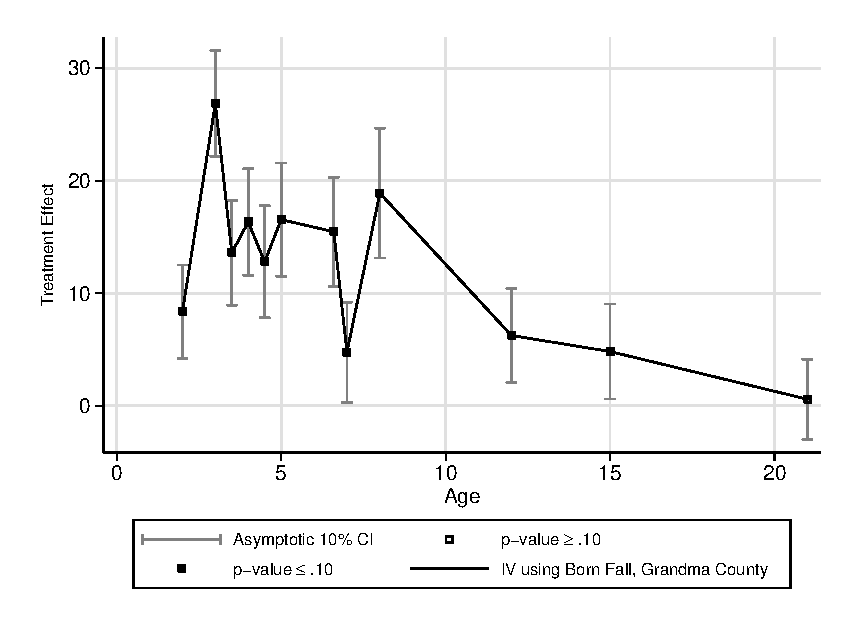
\includegraphics[width=.6\columnwidth]{output/appendixplots/main_iv_te.eps}
\floatfoot{
\footnotesize
\noindent Note: This plot presents the parameter associated with $D_i$ from an IV regression of $Y_i$ on $D_i$, $Q_i$, and $\mathbf{X}_i$, using $R_i$ and $\mathbf{Z_i}(1-R_i)$ as instruments. The outcomes ($Y_i$) are IQ tests at different ages, with a national standard deviation of 15 and a mean of 100. $\mathbf{X_i}$ includes a set of controls selected from all available baseline controls to maximize explanatory power across all outcomes tested in the paper: male, mother's IQ score, High-Risk Index, and Apgar Score at 1 minute. The confidence intervals are calculated at the 10\% significance level.}
\end{figure}

\begin{figure}[H]
		\caption{Effect of Center-based Preschool on Labor Market Outcomes, Accounting for Endogenous Take-up of Alternative Preschool Using Instrumental Variables} \label{fig:mainiv2}
		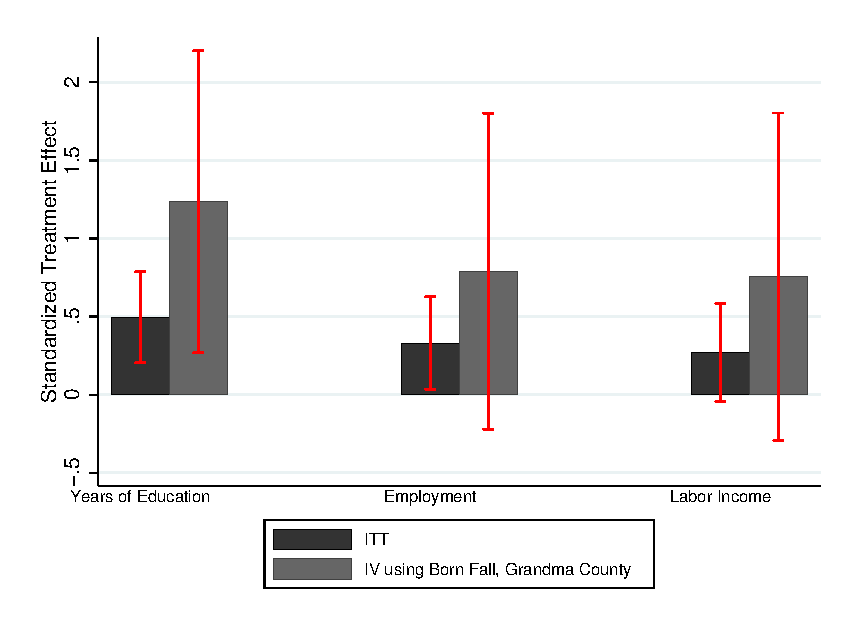
\includegraphics[width=.6\columnwidth]{output/appendixplots/main_iv_other.eps}
\floatfoot{
\footnotesize
\noindent Note: This plot presents the parameter associated with $D_i$ from an IV regression of $Y_i$ on $D_i$, $Q_i$, and $\mathbf{X}_{i}$, using $R_i$ and $\mathbf{Z}_{i}(1-R_i)$ as instruments. The outcomes ($Y_i$) are different relevant adult outcomes labeled in the horizontal axis. $\mathbf{X}_{i}$ includes a set of controls selected from all available baseline controls to maximize explanatory power across all outcomes tested in the paper: male, mother's IQ score, High-Risk Index, and Apgar Score at 1 minute. The confidence intervals are calculated at the 10\% significance level.}
\end{figure}

\subsubsection{Varying the Sets of Instruments}

\noindent Figure \ref{fig:ins_inter_Q_iv1} and Figure \ref{fig:ins_inter_Q_iv2} explore the sensitivity of the estimates to different sets of instruments. The pattern of results indicates that the method is generally robust to the three sets of instrumental variables that we consider. 

\begin{figure}[H]
		\caption{Effect of Center-based Preschool on IQ Scores, Accounting for Endogenous Take-up of Alternative Preschool Using Various Instrumental Variables} \label{fig:ins_inter_Q_iv1}
		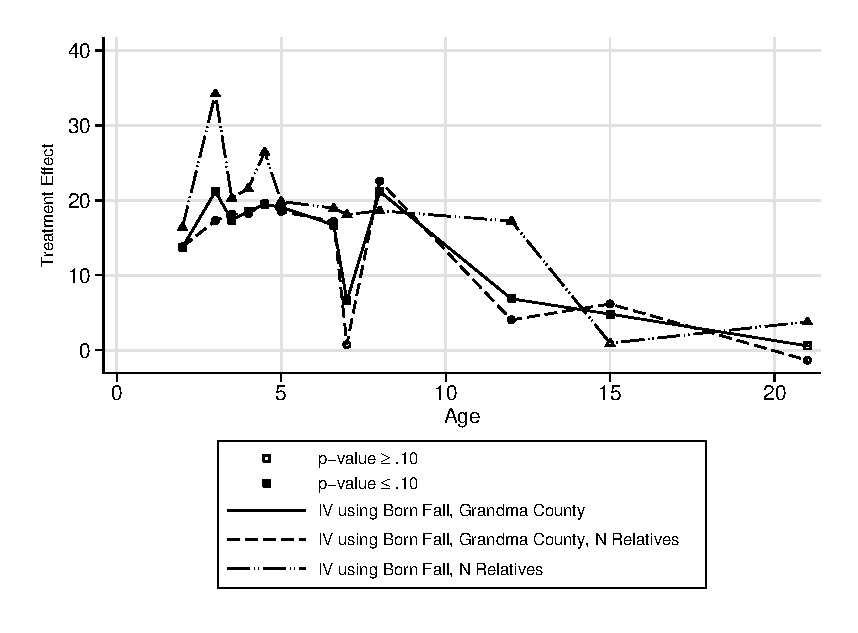
\includegraphics[width=.6\columnwidth]{output/appendixplots/ins_inter_Q_iv_te.eps}
\floatfoot{
\footnotesize
\noindent Note: This plot presents the parameter associated with $D_i$ from an IV regression of $Y_i$ on $D_i$, $Q_i$, and $\mathbf{X}_{i}$, using $R_i$ and $\mathbf{Z}_{i}(1-R_i)$ as instruments. The outcomes ($Y_i$) are IQ scores at different ages, with a national standard deviation of 15 and a mean of 100. $\mathbf{X_i}$ includes a set of controls selected from all available baseline controls to maximize explanatory power across all outcomes tested in the paper: male, mother's IQ score, High-Risk Index, and Apgar Score at 1 minute. The confidence intervals are calculated at the 10\% significance level.}
\end{figure}

\begin{figure}[H]
		\caption{Effect of Center-based Preschool on Labor Market Outcomes, Accounting for Endogenous Take-up of Alternative Preschool Using Various Instrumental Variables} \label{fig:ins_inter_Q_iv2}
		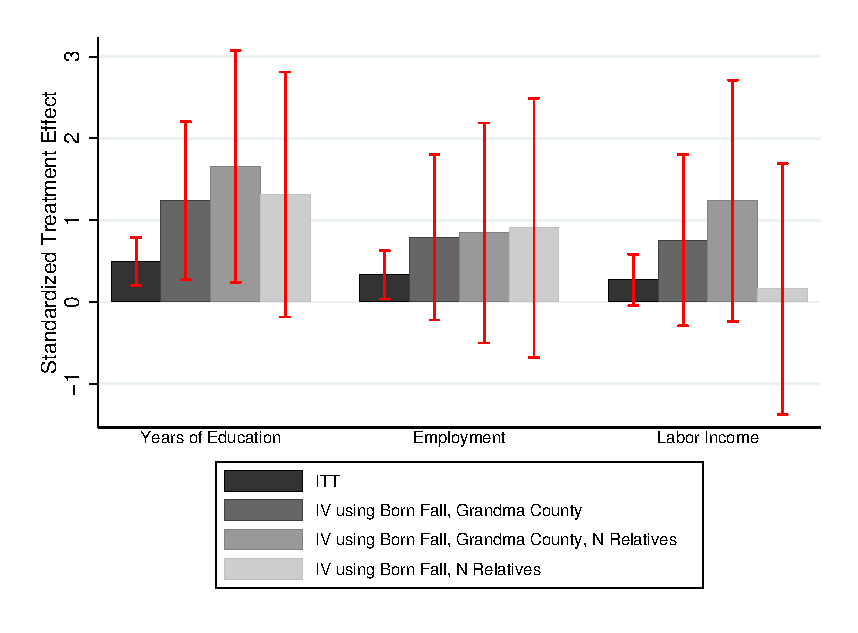
\includegraphics[width=.6\columnwidth]{output/appendixplots/ins_inter_Q_iv_other.eps}
\floatfoot{
\footnotesize
\noindent Note: This plot presents the parameter associated with $D_i$ from an IV regression of $Y_i$ on $D_i$, $Q_i$, and $\mathbf{X}_{i}$, using $R_i$ and $\mathbf{Z}_{i}(1-R_i)$ as instruments. The outcomes ($Y_i$) are different relevant adult outcomes labeled in the horizontal axis. $\mathbf{X}_{i}$ includes a set of controls selected from all available baseline controls to maximize explanatory power across all outcomes tested in the paper: male, mother's IQ score, High-Risk Index, and Apgar Score at 1 minute. The confidence intervals are calculated at the 10\% significance level.}
\end{figure}

\subsubsection{Varying the Specification of the Instruments}

\noindent We now present an exercise to evaluate the sensitivity of the results to different specifications of the instrumental variables. First, Figure~ \ref{fig:nointer_Q_iv} and Figure \ref{fig:nointer_Q_other} present the results using the set of instruments that are not interacted with an indicator for randomization into the control group ($1-R_i$). Figure \ref{fig:inter_Q_iv} and Figure \ref{fig:inter_Q_other} present results not only interacting the instruments but also interacting the observed characteristics we control for. In both exercises, we use $Q_i$ as the endogenous variable, along with $D_i$.\\

\noindent The results follow the same patterns as before, although they change when the instruments are not interacted. This makes economic sense because the interacted instruments better represent the economic intuition we offer before: the instruments other than $R_{i}$ are more likely to shift the decisions of the families of the control-group children compared to those of the treatment-group children.

\begin{figure}[H]
		\caption{Effect of Center-based Preschool on IQ Scores, Accounting for Endogenous Take-up of Alternative Preschool Using Various Instrumental Variables Specifications} \label{fig:nointer_Q_iv}
		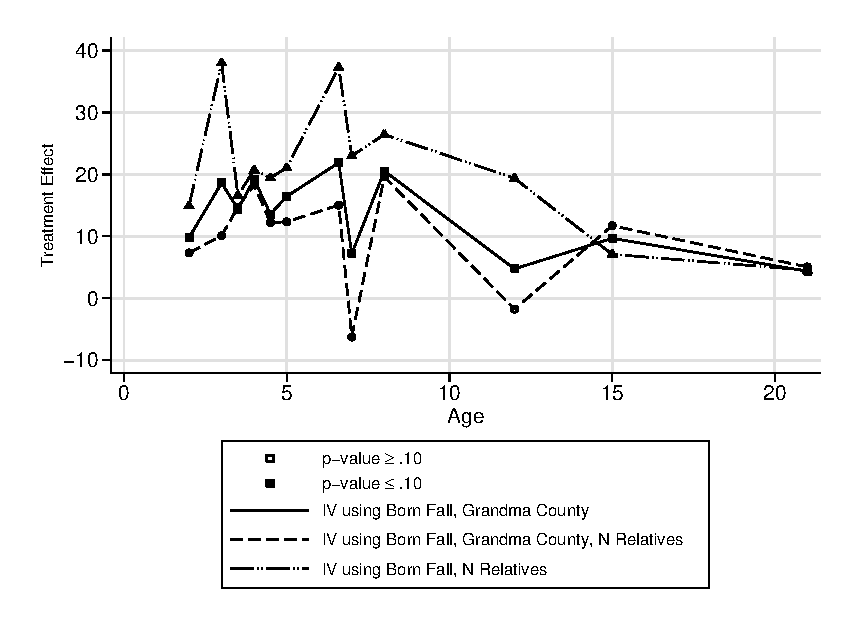
\includegraphics[width=.6\columnwidth]{output/appendixplots/nointer_Q_iv_te.eps}
\floatfoot{
\footnotesize
\noindent Note: This plot presents the parameter associated with $D_i$ from an IV regression of $Y_i$ on $D_i$, $Q_i$, and $\mathbf{X}_{i}$, using $R_i$ and $\mathbf{Z}_{i}$ as instruments. $Y_i$ is different IQ tests, with a national standard deviation of 15 and a mean of 100. $\mathbf{X_i}$ includes a set of controls selected from all available baseline controls to maximize explanatory power across all outcomes tested in the paper: Male, Mother's IQ, High-Risk Index, and APGAR Score at Age 1. The confidence intervals are calculated at the 10\% significance level.}
\end{figure}

\begin{figure}[H]
		\caption{Effect of Center-based Preschool on Labor Market Outcomes, Accounting for Endogenous Take-up of Alternative Preschool Using Various Instrumental Variables Specifications} \label{fig:nointer_Q_other}
		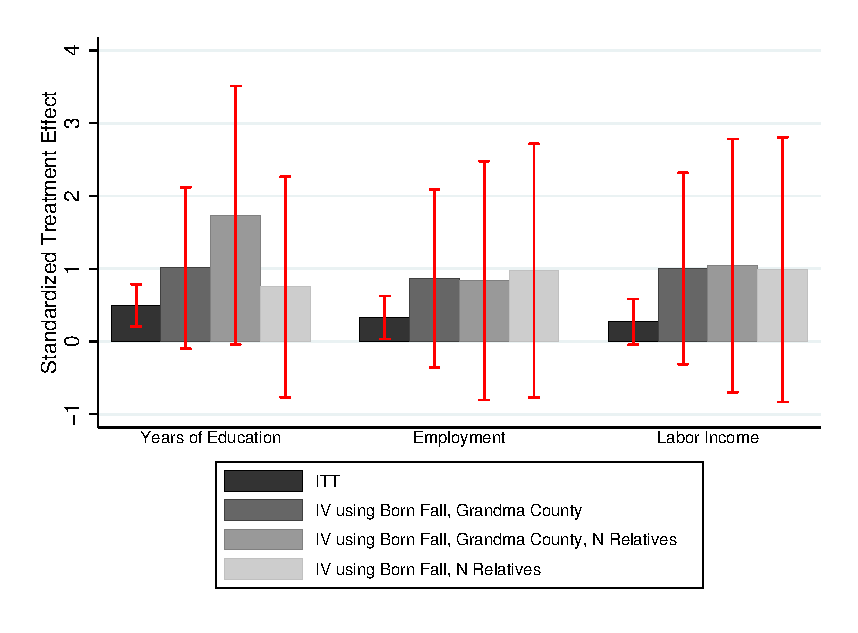
\includegraphics[width=.6\columnwidth]{output/appendixplots/nointer_Q_iv_other.eps}
\floatfoot{
\footnotesize
\noindent Note: This plot presents the parameter associated to $D_i$ from an IV regression of $Y_i$ on $D_i$, $Q_i$, and $\mathbf{X}_{i}$, using $R_i$ and $\mathbf{Z}_{i}$ as instruments. The outcomes ($Y_i$) are different relevant adult outcomes labeled in the horizontal axis. $\mathbf{X}_{i}$ includes a set of controls selected from all available baseline controls to maximize explanatory power across all outcomes tested in the paper: male, mother's IQ score, High-Risk Index, and Apgar Score at 1 minute. The confidence intervals are calculated at the 10\% significance level.}
\end{figure}

\begin{figure}[H]
		\caption{Effect of Center-based Preschool on IQ Scores, Accounting for Endogenous Take-up of Alternative Preschool Using Various Instrumental Variables Specifications} \label{fig:inter_Q_iv}
		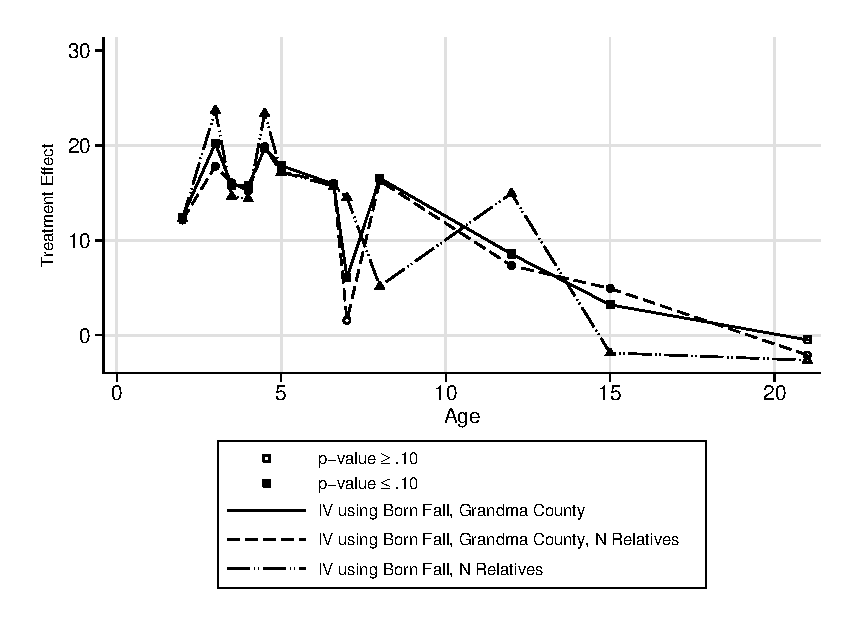
\includegraphics[width=.6\columnwidth]{output/appendixplots/inter_Q_iv_te.eps}
\floatfoot{
\footnotesize
\noindent Note: This plot presents the parameter associated with $D_i$ from an IV regression of $Y_i$ on $D_i$, $Q_i$ ,and $\mathbf{X}_{i}$, using $R_i$, $\mathbf{X}_{i}(1 - R_i)$ and $\mathbf{Z}_{i}(1 - R_i)$ as instruments. The outcomes ($Y_i$) are IQ scores at different ages, with a national standard deviation of 15 and a mean of 100. $\mathbf{X}_{i}$ includes a set of controls selected from all available baseline controls to maximize explanatory power across all outcomes tested in the paper: male, mother's IQ score, High-Risk Index, and Apgar Score at 1 minute. The confidence intervals are calculated at the 10\% significance level.}
\end{figure}

\begin{figure}[H]
		\caption{Effect of Center-based Preschool on Labor Market Outcomes, Accounting for Endogenous Take-up of Alternative Preschool Using Various Instrumental Variables Specifications} \label{fig:inter_Q_other}
		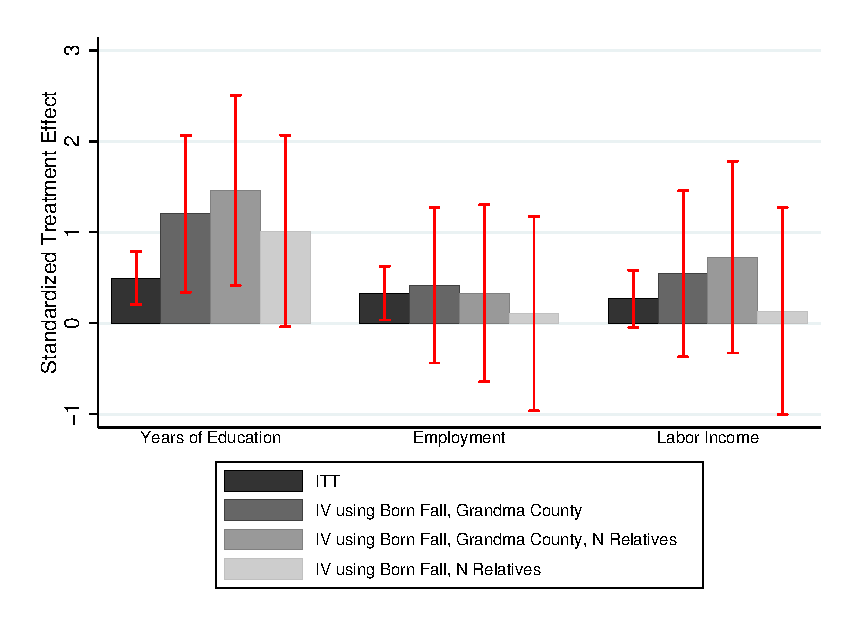
\includegraphics[width=.6\columnwidth]{output/appendixplots/inter_Q_iv_other.eps}
\floatfoot{
\footnotesize
\noindent Note: This plot presents the parameter associated with $D_i$ from an IV regression of $Y_i$ on $D_i$, $Q_i$, and $\mathbf{X}_{i}$, using $R_i$, $\mathbf{X}_{i}(1 - R_i)$ and $\mathbf{Z}_{i}(1 - R_i$) as instruments. The outcomes ($Y_i$) are different relevant adult outcomes labeled in the horizontal axis. $\mathbf{X}_{i}$ includes a set of controls selected from all available baseline controls to maximize explanatory power across all outcomes tested in the paper: male, mother's IQ score, High-Risk Index, and Apgar Score at 1 minute. The confidence intervals are calculated at the 10\% significance level.}
\end{figure}

\subsubsection{Varying the Parameterization of Alternative Preschool Take-up}

\noindent Now, we explore the sensitivity to the specification of $Q_{i}$ in \eqref{eq:ivnot}. We consider two alternatives. First, we use an indicator of take-up of alternative preschool, $P_{i}$ (Figure~\ref{fig:ins_inter_P_iv} and Figure~\ref{fig:ins_inter_P_other}). Second, we take the $\log$ of $Q_{i}$ (Figure~\ref{fig:ins_inter_LogQ_iv} and Figure~\ref{fig:ins_inter_LogQ_other}).

\begin{figure}[H]
		\caption{Effect of Center-based Preschool on IQ Scores, Accounting for an Endogenous Indicator of Take-up of Alternative Preschool} \label{fig:ins_inter_P_iv}
		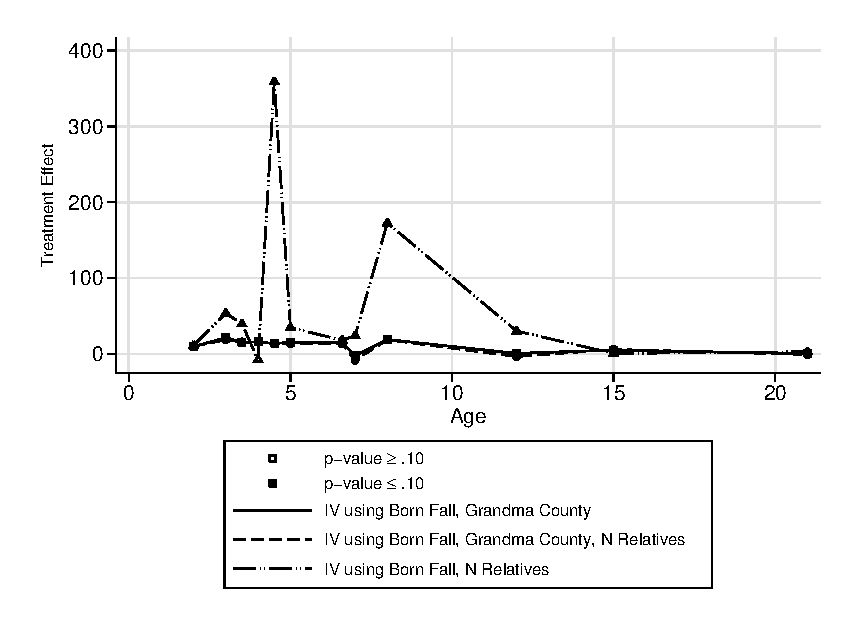
\includegraphics[width=.6\columnwidth]{output/appendixplots/ins_inter_P_iv_te.eps}
\floatfoot{
\footnotesize
\noindent Note: This plot presents the parameter associated with $D_i$ from an IV regression of $Y_i$ on $D_i$, $P_i$, and $\mathbf{X}_{i}$, using $R_i$, $\mathbf{Z}_{i}(1 - R_i)$ as instruments. The outcomes ($Y_i$) are IQ scores at different ages, with a national standard deviation of 15 and a mean of 100. $\mathbf{X}_{i}$ includes a set of controls selected from all available baseline controls to maximize explanatory power across all outcomes tested in the paper: male, mother's IQ score, High-Risk Index, and Apgar Score at 1 minute. The confidence intervals are calculated at the 10\% significance level.}
\end{figure}

\begin{figure}[H]
		\caption{Effect of Center-based Preschool on Labor Market Outcomes, Accounting for an Endogenous Indicator of Take-up of Alternative Preschool} \label{fig:ins_inter_P_other}
		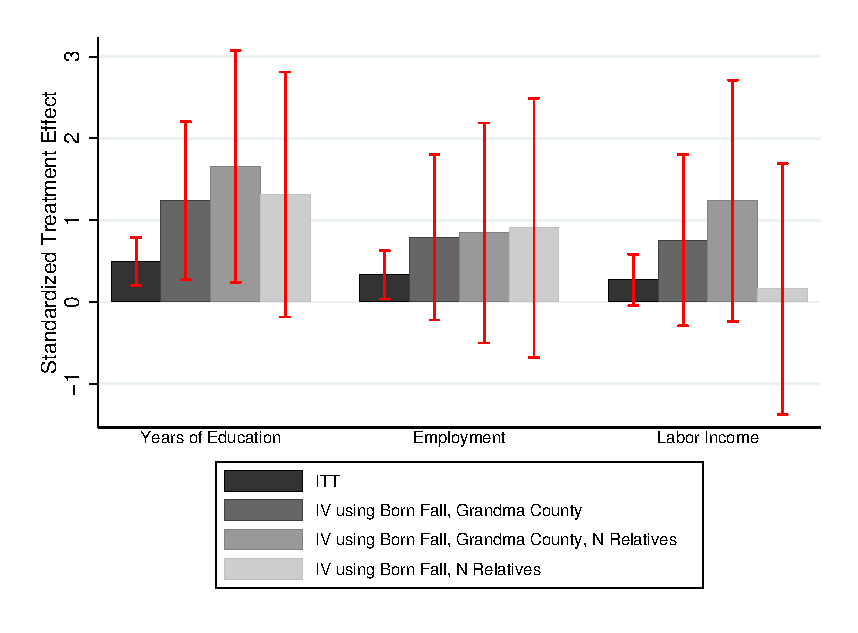
\includegraphics[width=.6\columnwidth]{output/appendixplots/ins_inter_P_iv_other.eps}
\floatfoot{
\footnotesize
\noindent Note: This plot presents the parameter associated to $D_i$ from an IV regression of $Y_i$ on $D_i$, $P_i$, and $\mathbf{X}_{i}$, using $R_i$, $\mathbf{Z}_{i}(1 - R_i$) as instruments. The outcomes ($Y_i$) are different relevant adult outcomes labeled in the horizontal axis. $\mathbf{X}_{i}$ includes a set of controls selected from all available baseline controls to maximize explanatory power across all outcomes tested in the paper: male, mother's IQ score, High-Risk Index, and Apgar Score at 1 minute. The confidence intervals are calculated at the 10\% significance level.}
\end{figure}

\begin{figure}[H]
		\caption{Effect of Center-based Preschool on IQ Scores, Accounting for Endogenous (log) Months of Take-up of Alternative Preschool} \label{fig:ins_inter_LogQ_iv}
		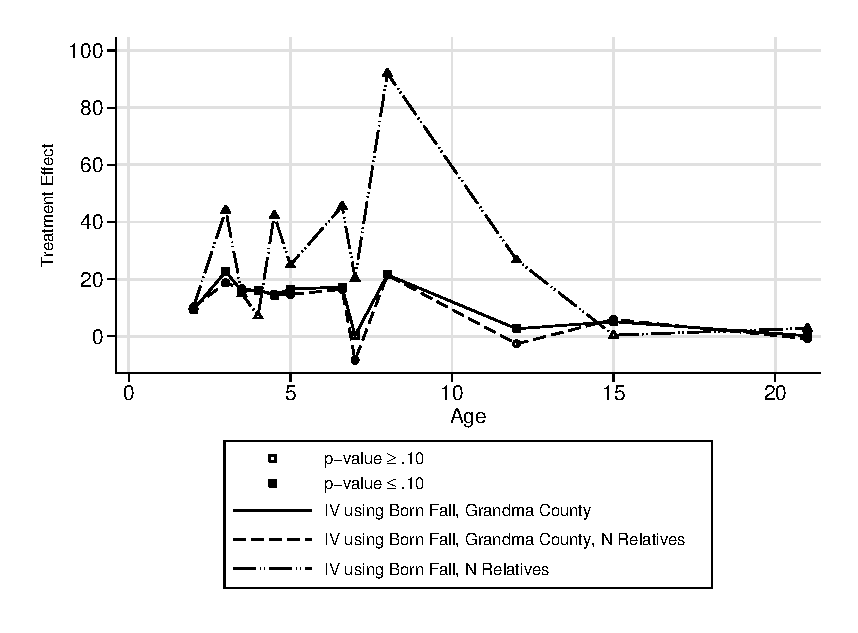
\includegraphics[width=.6\columnwidth]{output/appendixplots/ins_inter_logQ_iv_te.eps}
\floatfoot{
\footnotesize
\noindent Note: This plot presents the parameter associated with $D_i$ from an IV regression of $Y_i$ on $D_i$, $\log Q_i$, and $\mathbf{X}_{i}$, using $R_i$, $\mathbf{Z}_{i}(1 - R_i)$ as instruments. The outcomes ($Y_i$) are IQ scores at different ages, with a national standard deviation of 15 and a mean of 100. $\mathbf{X}_{i}$ includes a set of controls selected from all available baseline controls to maximize explanatory power across all outcomes tested in the paper: male, mother's IQ score, High-Risk Index, and Apgar Score at 1 minute. The confidence intervals are calculated at the 10\% significance level.}
\end{figure}

\begin{figure}[H]
		\caption{Effect of Center-based Preschool on Labor Market Outcomes, Accounting for Endogenous (log) Months of Take-up of Alternative Preschool} \label{fig:ins_inter_LogQ_other}
		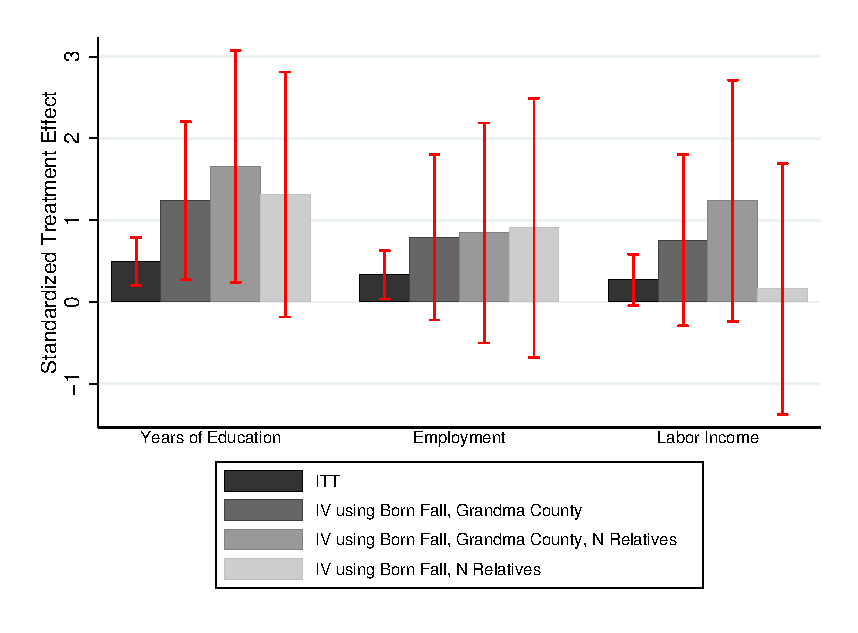
\includegraphics[width=.6\columnwidth]{output/appendixplots/ins_inter_logQ_iv_other.eps}
\floatfoot{
\footnotesize
\noindent Note: This plot presents the parameter associated with $D_i$ from an IV regression of $Y_i$ on $D_i$, $\log Q_i$, and $\mathbf{X}_{i}$, using $R_i$, $\mathbf{Z}_{i}(1 - R_i$) as instruments. The outcomes ($Y_i$) are different relevant adult outcomes labeled in the horizontal axis. $\mathbf{X}_{i}$ includes a set of controls selected from all available baseline controls to maximize explanatory power across all outcomes tested in the paper: male, mother's IQ score, High-Risk Index, and Apgar Score at 1 minute. The confidence intervals are calculated at the 10\% significance level.}
\end{figure}


\subsection{Control Functions}

\noindent We now consider a control function approach. With control functions, the objective is also to simultaneously account for take-up of center-based childcare and  alternatives. 

\subsubsection{Setup}

\noindent The method we propose is an application of the selection correction in \citet{Heckman_1979_Econometrica}. We model the selection into both endogenous variables of interest, center-based childcare and preschool alternatives. The method involves three equations: (i) the outcome equation; (ii) the probability of participating in center-based childcare; (iii) a linear equation describing the number of months enrolled in preschool alternatives.\\

\noindent Let $Y^{0}_{i}$ be the counterfactual outcome of child $i$ when not participating in center-based childcare. Similarly, let $Y^{1}_{i}$ be her potential outcome if she participates. We model the outcome as: 
 
\begin{eqnarray}
Y_{i}^1 &=& \alpha^1+\mathbf{X}_{i} \mathbf{\beta}                 +\varepsilon_i^1 \nonumber  \\
Y_{i}^0 &=& \alpha^0+\mathbf{X}_{i} \mathbf{\beta} + \alpha^Q Q_i+\varepsilon_i^0.  \label{eq:potout}
\end{eqnarray}

\noindent The equation describing participation in center-based childcare is: 

\begin{equation}
D_{i} = \left\{
        \begin{array}{ll}
        	0 &\text{if } D_{i}^* \leq  0 \\
            1 &\text{if } D_{i}^* > 0, \label{eq:sel1}
        \end{array}
    \right. 
\end{equation}

\noindent where we interpret $D_{i}^*$ as a latent continuous variable representing the household's interest in sending the child to treatment. We write

\begin{equation}
D^{*}_i = \mathbf{W}_i \gamma^{D} + \varepsilon^{D}_i, \label{eq:probitD}
\end{equation}

\noindent where $\mathbf{W}_i$ is a vector that includes $\mathbf{X}_i$ and $R_i$ and can include variables that shift the decision to enroll children into ABC or CARE without shifting the counterfactual outcome of interest, $Y^{d}_{i}$. \\

\noindent We write the selection equation into months of preschool as a linear equation with fixed coefficients, assuming homogeneous treatment effects:

\begin{equation}
Q_i = \mathbf{W}_i \gamma^{Q} + \varepsilon^{Q}_i, \label{eq:selq}
\end{equation}

\noindent In general, the unobserved variables in each of these equations are correlated. We assume that they are distributed as follows: 

\begin{equation}
        \left[ \begin{array}{l}
        	 \varepsilon_{i}^1 \\
            \varepsilon_{i}^0 \\
            \varepsilon_{i}^D
        \end{array} \right]  \sim \mathcal{N} \left[ \left( \begin{array}{l}
        	 0 \\
           0 \\ 
           0
        \end{array} \ \right), 
                \left( \begin{array}{llll}
        	 \sigma_{1}^2 & \sigma_{1,0} & \sigma_{1,D}   \\
             \sigma_{1,0} & \sigma_{0}^2 & \sigma_{0,D}   \\
             \sigma_{1,D} & \sigma_{0,D} & 1 
        \end{array} \right) \right],  \label{eq:udist}
\end{equation}

\noindent where we normalize $\var \left( \varepsilon^D_i \right) =1$.\\

\noindent Further, we assume that 
\begin{equation}
\mathbb{E}\left[\varepsilon_i^0|D_i=0,\mathbf{W}_i,\varepsilon^{Q}_i,Q_i=q\right]=\sigma^{0Q}\varepsilon^{Q}_i+\mathbb{E}\left[\varepsilon_i^0|D_i=0,\mathbf{W}_i\right].
\label{eq:E[epsilon0]}
\end{equation}

\subsubsection{Identification}

\noindent The following steps identify the parameters of interest. First, we estimate the parameters characterizing the decision to enroll the child in center-based childcare. We exploit the assumption that $\varepsilon_{i}^D \sim \mathcal{N} \left( 0, 1 \right)$ in \eqref{eq:udist} and estimate the parameters in \eqref{eq:probitD} using a probit model.\\

\noindent Second, we approximate the unobserved term relevant to the choice of $Q_{i}$. We take the coefficients in \eqref{eq:selq} to obtain an estimate for $\varepsilon^{Q}_i$. By linearly conditioning on this term, we account for the correlation between the error term in the decision for $Q_{i}$ and the error term in the outcome equation, $\varepsilon_i^0$.\\

\noindent Third, we estimate the coefficients in the outcome equation using the proxies for the unobserved components. We rewrite \eqref{eq:potout} using conditional expectations:

\begin{eqnarray}
\mathbb{E}\left[Y_i^1|D_i=1,\mathbf{W}_i\right]                         &=& \alpha^1+\mathbf{X}_i\mathbf{\beta}              +\mathbb{E}\left[\varepsilon_i^1|D_i=1,\mathbf{W}_i      \right] \nonumber \\
\mathbb{E}\left[Y_i^0|D_i=0,\mathbf{W}_i,\varepsilon^{Q}_i,Q_i=q\right] &=& \alpha^0+\mathbf{X}_i\mathbf{\beta} +\alpha^Q q \label{eq:condout} \\ \nonumber && \quad + \mathbb{E}\left[\varepsilon_i^0|D_i=0,\mathbf{W}_i,\varepsilon^{Q}_i,Q_i=q\right].
\end{eqnarray}

\noindent Once we condition on the proxy for $\varepsilon^{Q}_i$, the error term in the outcome equations only depends on the selection into center-based childcare. The conditional error terms in equation \eqref{eq:condout} can be specified as control functions.\\ 

\noindent For children enrolled in treatment, the control function is: 
\begin{equation}
\mathbb{E} \left[\varepsilon_i^1|D_i=1,\mathbf{W}_i \right]=\sigma_1\frac{\phi \left( \mathbf{W}_i \gamma^D \right) }{ \Phi \left( \mathbf{W}_i \gamma^D \right) }. \label{eq:contam}
\end{equation}

\noindent For children not enrolled in the treatment, the control function is:
\begin{equation}
\mathbb{E} \left[\varepsilon_i^0|D_i=0,\mathbf{W}_i,\varepsilon^{Q}_i,Q_i=q\right]= \sigma^{0Q}\varepsilon^{Q}_i - \sigma_0 \frac{\phi\left(\mathbf{W}_i\gamma^D\right)}{\Phi\left( - \mathbf{W}_{i} \gamma^D \right) }. \label{eq:home}
\end{equation}

\subsection{Estimates}

\noindent By including the control functions, we can recover consistent estimates of the parameters in \eqref{eq:potout} through a linear regression. The childcare is the difference of the intercepts in the two outcome equations.\\

\noindent The charts below present the estimates for the parameter associated with $D_i$. That is, the effect of participating in center-based childcare relative to a counterfactual of receiving no preschool alternative. As before, we present results for IQ scores at different ages and for a set of relevant adult outcomes. The results are not compelling, as they present irregularities over the life-cycle that differ from the rest of results we present in the main paper and throughout this appendix. 

\begin{figure}[H]
		\caption{Effect of Center-based Preschool on IQ Scores, Accounting for Endogenous (log) Months of Take-up of Alternative Preschool} \label{output/appendixplots/Q_cf_te.eps}
		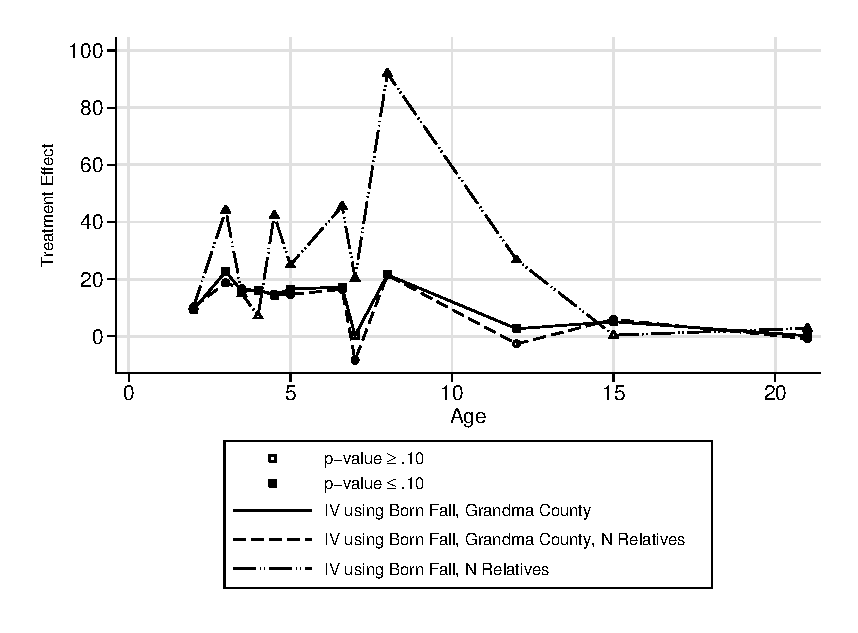
\includegraphics[width=.6\columnwidth]{output/appendixplots/ins_inter_logQ_iv_te.eps}
\floatfoot{
\footnotesize
\noindent Note: This plot presents the parameter associated with $D_i$ estimated using Control Functions as described in the text. The outcomes ($Y_i$) are IQ scores at different ages with a national standard deviation of 15 and a mean of 100.  $D_i=1$ for children that participate in ABC or CARE center-based treatment, and $D_i=0$ for children who do not participate in treatment. $Q_i$ is the number of months attending preschool. It is coded as zero for children participating in ABC or CARE. $\mathbf{X}_{i}$ includes a set of controls selected from all available baseline controls to maximize explanatory power across all outcomes tested in the paper: male, mother's IQ score, High-Risk Index, and Apgar Score at 1 minute.}
\end{figure}

\begin{figure}[H]
		\caption{Effect of Center-based Preschool on Labor Market Outcomes, Accounting for Endogenous (log) Months of Take-up of Alternative Preschool} \label{output/appendixplots/Q_cf_te.eps}
		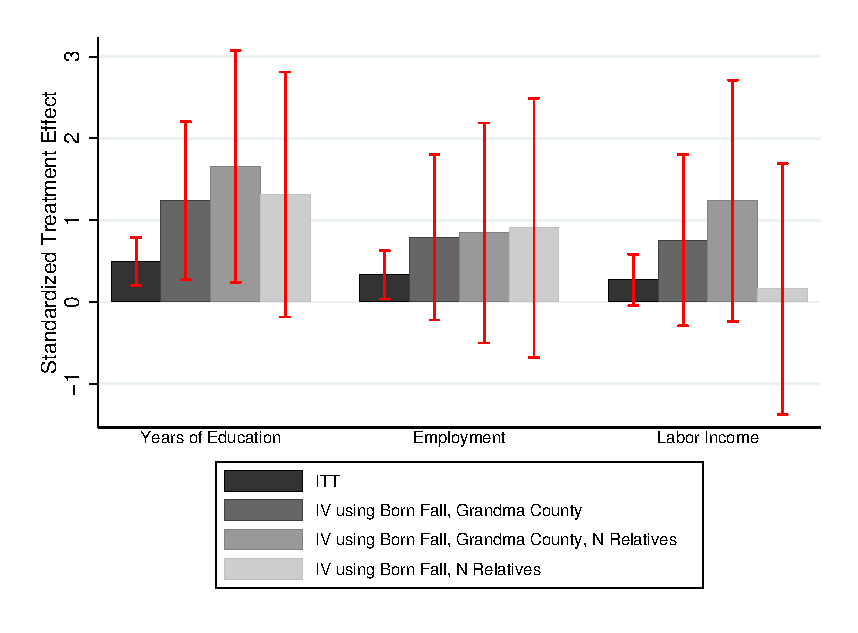
\includegraphics[width=.6\columnwidth]{output/appendixplots/ins_inter_logQ_iv_other.eps}
\floatfoot{
\footnotesize
\noindent Note: This plot presents the parameter associated with $D_i$ estimated using Control Functions as described in the text. The outcomes ($Y_i$) are different relevant adult outcomes labeled in the horizontal axis.  $D_i=1$ for children that participate in ABC or CARE center-based treatment, and $D_i=0$ for children who do not participate in treatment. $Q_i$ is the number of months attending. It is coded as zero for children participating in ABC or CARE. $\mathbf{X}_{i}$ includes a set of controls selected from all available baseline controls to maximize explanatory power across all outcomes tested in the paper: male, mother's IQ score, High-Risk Index, and Apgar Score at 1 minute.}
\end{figure}

\setcounter{figure}{0}  \renewcommand{\thefigure}{E.\arabic{figure}}
\setcounter{table}{0}   \renewcommand{\thetable}{E.\arabic{table}}
\section{Assessing Common Critiques to ABC} \label{appendix:assessingcc}

\noindent This section of the appendix assesses some of the critiques to ABC, which could apply to CARE as well. The critiques focus on the first phase of the program, to which we refer simply as ABC in this section of the appendix. We consider the following categories of critiques: (i) validity of treatment effects given early differences between treatment and control groups, (ii) fadeout of the treatment effect on cognitive outcomes, and (iii) compromised randomization. \\

\subsection{Treatment Effects vs. Early Differences Between Groups}

\noindent The first critique we assess is that of \citet{Spitz_1992_ABC-Retardation}. The author asks if ABC prevented socio-cultural mental retardation. He focuses on different measures of cognition, and generically calls them IQ. His main focus is on the raw mean difference between the treatment and the control groups in the Bayley Mental Development Index (MDI) from the Bayley Scales of Infant Development and Infant Behavior (BSID) at 1 year of age.\footnote{The Bayley Mental Development Index (MDI) is a standard measure of cognition at taken between ages 0 and 2 \citep{Childrens-Health_2016_Bayley-Scales}.} He finds a noticeable disparity in the mean difference between cohorts 1 and 2 and cohorts 3 and 4, as early as six months after the treatment began. As \citet{Spitz_1992_ABC-Retardation} argues, this difference is conspicuous and we display it in Table~\ref{table:cohorts}. Importantly, the author fails to note that the mean differences have noticeably high standard errors.

\begin{table}[H] 
\begin{threeparttable}
\caption{Treatment - Control Mean Difference by Cohort, ABC}
\label{table:cohorts}
\centering 
\begin{tabular}{lcc} \toprule
 & (1) & (2) \\
 & Bayley MDI, 12 Months & Bayley MDI, 24 Months \\ \midrule
 &  &  \\\
Cohort 1 & 4.841 & -2.901 \\
 & (6.013) & (5.926) \\
Cohort 2 & 0.071 & 1.882 \\
 & (6.013) & (5.830) \\
Cohort 3 & 9.143 & 10.038 \\
 & (5.801) & (5.926) \\
Cohort 4 & 7.829 & 13.713 \\
 & (5.801) & (5.830) \\ \\ \midrule
Observations & 112 & 110 \\
$R^2$ & 0.055 & 0.110 \\ \bottomrule
 \end{tabular}
\begin{tablenotes}
\footnotesize
\item Note: This table displays the mean difference between the treatment and control groups in two measures of the Bayley Mental Development Index, for ABC. Homoskedastic, asymptotic standard errors are in parentheses.
\end{tablenotes}
\end{threeparttable}
\end{table}

\noindent \citet{Spitz_1992_ABC-Retardation} states that: ``an essential question is whether the differences at 6 months of age were due to the intervention or were preexisting'' \citep[][p. 230]{Spitz_1992_ABC-Retardation}. \citet{Spitz_1992_ABC-Retardation} proceeds with speculative exercises that lead him to state that it is questionable to conclude that the mean difference between the treatment and control groups as early as 6 months of age is a consequence of the treatment.\footnote{The exact quote is: ``Even if the differences between experimental and control groups at 6 months of age were a consequence of the first few months of intervention, which is questionable, the negligible additional effects after age 4.5 more years in the program should at least make one cautious about this kind of intervention's potential [\ldots]'' \citep[][p. 235]{Spitz_1992_ABC-Retardation}. We assess the former point before getting to the latter.}\\

\noindent His argument stems from not receiving information on the maternal characteristics, which he considers fundamental for his analysis to comparing test scores over the years.\footnote{He does not note that tests scores \textit{do not have a well-defined scale} and are hard to compare.}\\ 

\noindent We present some annotations with respect to the comments in \citet{Spitz_1992_ABC-Retardation}.\\ 

\noindent \textbf{1. Mothers do not significantly differ in observed characteristics between the treatment and the control groups in any ABC cohort.} When jointly testing the hypothesis of differences in a battery of observed characteristics, we fail to reject any difference between the families of these children (see Table~\ref{tab:baseline_coh1} to Table~\ref{tab:baseline_coh4}). Even when the point estimates present some differences, they are minimal. For example, treatment-group mothers differ from control-group mothers, on average, by having one point higher IQ score (the population standard deviation is 15 points).\\

\noindent \textbf{2. Other early childhood education programs have generated gains in cognition very early in life, as soon as a year after the start of the program.} A more recent program, the Infant Health and Development Program (IHDP), treated children from ages 0 to 3. \citet{Gross_Spiker_etal_1997_BOOKHelpinglowbirth} thoroughly describe this program. A lot of its elements were based on ABC and CARE. The program offered, on average, eight hours a week of center-based childcare from ages 1 to 3, weekly home visits from ages 0 to 1, and bi-monthly home visits from ages 1 to 3. Measures of the Bayley MDI at 12 and 24 months are available. The most intensive part of the treatment, center-based childcare, began in IHDP at 12 months of age while it began in ABC at birth. As in ABC, after a few months of center-based childcare, the effects on cognition were substantial in IHDP.

\begin{table}[H] 
\begin{threeparttable}
\caption{Treatment - Control Mean Difference, IHDP}
\label{table:ihdp}
\centering 
\begin{tabular}{lcc} \hline \hline
 & (1) & (2) \\
 & Bayley MDI, 12 Months & Bayley MDI, 24 Months \\ \hline
 &  &  \\\
Mean Treatment - Mean Control & 0.142 & 9.958 \\
 & (0.968) & (1.498) \\
 &  &  \\ \hline
Observations & 893 & 910 \\
$R^2$ & 0.000 & 0.067 \\ \hline \hline  
\end{tabular}
\begin{tablenotes}
\footnotesize
\item Note: This table displays the mean difference between the treatment and control groups in two measures of the Bayley Mental Development Index, for the Infant Health and Development Program using the principal analysis sample. Robust standard errors clustered by state and an indicator of weight below 2,000 grams in parentheses.
\end{tablenotes}
\end{threeparttable}
\end{table}


\noindent \textbf{3. The effects on cognition are sustained throughout childhood and up to age 21 even when partialing out the Bayley MDI at ages 12 and 24 months.} When partialing out from a linear regression the score in the Bayley MDI tests both at 12 and 24 months of age, the treatment effects on cognition, measured by the mean difference in IQ scores at different ages between the treatment and control groups, are still significant and are sustained up to age 21 (see Figure~\ref{fig:treatiqsabc}).

\begin{figure}[H]
		\caption{Treatment Effects on IQ, ABC} \label{fig:treatiqsabc}
		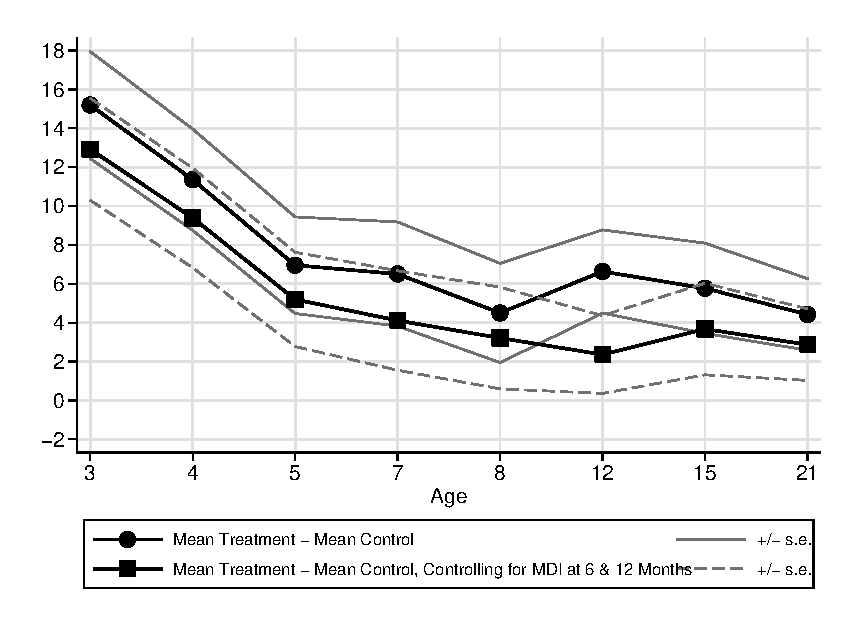
\includegraphics[width=.9\columnwidth]{output/abc_mdifixing_2.eps}
\floatfoot{
\footnotesize
\noindent Note: This figure displays the mean difference in IQ scores at different ages between the treatment and control groups, pooling males and females. The line with circles represents the raw difference. The line with squares represents the difference when linearly controlling for the Bayley Mental Development Index at 6 and 12 months.}
\end{figure}

\noindent The author raises an additional concern. He states that even if the early-life effects on the Bayley MDI were true, the effects were not long-lasting. When doing so, he exclusively refers to the effects the program had on cognition. As we document throughout the main paper, however, ABC had effects on a wide set of life-cycle outcomes, which perhaps are more important than the effects on cognition if measured by the economic gains they generate. Examples include: employment at age 30 for males, high-school graduation for females, and a variety of health measures at age 34 for males. We document these effects in the main paper.\\

\subsection{Fadeout of Treatment Effects}

\noindent This sustained effect on life-cycle outcomes relates to another category of criticism of ABC---the fadeout of treatment effects after the actual treatment period.\footnote{See, for example, \citet{Besharov-etal_2011_ABCProject}.} Based on the fadeout of the effects on cognition and age-21 outcomes, some studies claim that ABC had no sustained long-term effects. In addition to the evidence we cite above, it is important to add the following.\\

\noindent  \textbf{4. The treatment effects of ABC differed by gender.} For example, we find substantial effects on employment for males and high-school graduation for females. This does not mean that the program did not work. It means that market conditions could have affected the way in which the treated subjects could have benefited from the program's effects.\\

\subsection{Compromised Randomization}

\begin{sidewaystable}[H] 
\begin{threeparttable}
\caption{Randomization Compromises, ABC}
\label{table:abccompromises}
\centering
\footnotesize
\begin{tabular}{ccccc} \toprule
Child ID & Initial Assignment & Compromise Description & Data Availability & Methodology Assumption \\ \\ \midrule
Case A & Treatment & Left the study & None & Missing at random \\
Case B & Treatment & Left the study & None & Missing at random \\
Case C & Treatment & Left the study & None & Missing at random \\
Case D & Treatment & Left the study & None & Missing at random \\ \midrule
.x    & Control  & Died (age 0), heart disease & Baseline; before dead & Attrition after death \\
914 & Control  & Died (age 0), heart disease & Baseline; before dead & Attrition after death \\
74 & Treatment & Died (age 0), SIDS & Baseline; before dead & Attrition after death \\
99 & Treatment  & Died (age 4), pedestrian accident & Baseline; before dead & Attrition after death \\ \midrule
900 & Treatment  & Non-compliance  & Baseline; before age 8 & Attrition after age 8  \\
912 & Treatment  & Non-compliance  & Baseline; before age 8 & Attrition after age 8  \\
922 & Treatment  & Non-compliance  & Baseline; before age 8 & Attrition after age 8  \\ \midrule
78  & Control        & Crossover from control to treatment & Baseline; before age 8 & Attrition after age 8  \\ \midrule
85 & Treatment   & 3 months of treatment &  Baseline; after age 2 & Same as treatment group  \\  
103 & Treatment &10 months of treatment &  Baseline; after age 2 & Same as treatment group  \\
108 & Treatment & 6 months of treatment &  Baseline; after age 2 & Same as treatment group  \\ 
123 & Treatment & 9 months of treatment &  Baseline; after age 2 & Same as treatment group  \\  \midrule
906 & Control  & Left study at 54 months & Baseline; before 54 months & Attrition after 54 months \\ \midrule
95   & Treatment       & Developmentally delayed at 6 months & No data after diagnosis & Dropped (non-eligible) \\ 
124 & Treatment       & Developmentally delayed at 36 months & No data after diagnosis & Dropped (non-eligible) \\ \midrule
 82 & Control       & Crossover from control to treatment & Baseline, before age 8 & Dropped (non-eligible)  \\ 
 119 & Control       & Crossover from control to treatment & Baseline, before age 8 & Dropped (non-eligible)  \\ \bottomrule
\end{tabular}
\begin{tablenotes}
\item Note: This table describes the various randomization compromises in ABC. For each child, we display: the ID assigned by the program staff, the nature of the compromise, the data available, and the methodological assumption when accounting for non-compliance and program attrition. 
\end{tablenotes}
\end{threeparttable}
\end{sidewaystable}

\noindent The third and last critique we assess is that of compromised randomization.\footnote{See for example \citet{Baumeister-Bacharach_2000_Early-Generic} and the multiple studies cited there.} The main critique to the program in this respect is that seven children in the treatment group did not comply to their initial assignment and one child switched from control to treatment status. This critique refers to the children labeled with the following IDs by the program: Case A, Case B, Case C, Case D, 900, 912, 922, 78, 82, and 119 (see Table~\ref{table:abccompromises}, which we reproduce from the main paper). Although we document more cases of compromised randomization, we start by assessing these eight cases.\footnote{Our main methodology assesses all the cases except the children for whom we do not have data at all (Case A, Case B, Case C, Case D). We are not able to account for them because our method is based on observing at least some baseline characteristics. See Section~\ref{section:methodology} in the main paper for more details.}\\

\noindent First, we propose a method to assess the non-compliance of children 900, 912, 922, 78, 82, and 119 for whom we have data available from ages 0 to 8. This allows for the possibility to adjust the mean difference between the treatment and the control groups, using a standard Bloom estimator \citep{Bloom_1984_ER}. This estimator accounts for compliance, by weighting the mean difference by a measure of the probability of compliance. It takes the following form: 

\begin{equation}
\Delta^{\textbf{Bloom}} = \frac{\mathbb{E} \left[ Y | R = 1 \right] - \mathbb{E} \left[ Y | R = 0 \right] }{\mathbb{E} \left[ D | R = 1 \right] - \mathbb{E} \left[ D | R = 0 \right]}, 
\end{equation}

\noindent where $R$ indicates randomization into treatment, $D$ indicates treatment take-up, and $Y$ is an outcome of interest.\\

\noindent This estimator coincides with the instrumental variable estimator of the parameter in a linear regression of an outcome on a single explanatory variable, e.g. treatment take-up. As \citet{Angrist_Imbens_ea_1996_JASA} show, under certain assumptions it can be interpreted as the average treatment effect for those individuals induced to take up treatment by the instrument. This interpretation has various weaknesses \citep{Heckman_Urzua_etal_2006_REStat,Heckman_Urzua_2010_JoE}.\\

\noindent To compare the mean difference and the Bloom estimator we consider two measures of cognition, which are commonly used when evaluating ABC and are available for children 900, 912, 922, 78, 82, 119: the Stanford-Binet Intelligence Scale at age 3 and the Wechsler Preschool and Primary Scale of Intelligence at age 5. Table~\ref{table:nc1} presents the results and shows that the differences are minimal. \textbf{5. Adjusting for the non-compliance of children 900, 912, 922, 78, 82, and 119 makes little difference} when assessing outcomes for which we observe these children. 

\begin{table}[H] 
\begin{threeparttable}
\caption{Assessing Non-compliance in ABC, Exercise 1}
\label{table:nc1}
\centering 
\begin{tabular}{ccccc} \toprule
 & (1) & (2) & (3) & (4) \\
 & IQ, Age 3 & IQ, Age 3  & IQ, Age 5 & IQ, Age 5 \\ \midrule
 &  &  & & \\\
Treatment - Control Mean Difference & 14.970 &  & 6.398 &  \\
 & (2.794) &  & (2.494) &  \\
Bloom &  & 16.245 &  & 6.943 \\
 &  & (2.877) &  & (2.643) \\ \midrule
Observations & 100 & 100 & 100 & 100  \\
 $R^2$ & 0.227 & 0.289 & 0.063 & 0.088 \\ \bottomrule
 \end{tabular}
\begin{tablenotes}
\footnotesize
\item Note: This table displays the mean difference between the treatment and control groups and the same difference adjusted for non-compliance (Bloom estimator) in two measures of IQ, the Stanford-Binet IQ Score at age 3 and the Wechsler Preschool and Primary Scale of Intelligence at age 5. Homoskedastic, asymptotic standard errors are in parentheses.
\end{tablenotes}
\end{threeparttable}
\end{table}


\noindent Second, we propose a method to account for non-compliance of the children Case A, Case B, Case C, Case D. For them, we have no data at all. We reproduce the estimates in Table~\ref{table:nc2}, assigning the lowest score across all the children in the treatment group to each of these four children. For each of the tests we consider, the lowest score was 71 for both the age-3 and the age-5 measures. \textbf{6. Even when assigning the worst score to the children who did not comply to treatment and for whom no data is available, the mean difference between treatment and control is sizable and not significantly different from the baseline cases where we do not adjust for non-compliance cases} (columns (1) and (3) in Table~\ref{table:nc1}).

\documentclass[]{article}
\setlength{\pdfpagewidth}{8.5in} \setlength{\pdfpageheight}{11in}
\begin{document}
\begin{tabular}{lcccc} \hline
 & (1) & (2) & (3) & (4) \\
 & iq3y\_itt & iq3y\_iv & iq5y\_itt & iq5y\_iv \\
VARIABLES & IQ at age 3y months & IQ at age 3y months & IQ at age 5y months & IQ at age 5y months \\ \hline
 &  &  &  &  \\
Randomization into center-based care (ABC and CARE) & 12.908*** &  & 4.284 &  \\
 & (2.901) &  & (2.647) &  \\
Indicator for the actual treatment receipt for center-based care &  & 15.111*** &  & 5.016* \\
 &  & (3.061) &  & (2.960) \\
 &  &  &  &  \\
Observations & 104 & 104 & 104 & 104 \\
 R-squared & 0.163 & 0.306 & 0.025 & 0.093 \\ \hline
\end{tabular}
\end{document}


\noindent Finally, we note that our methodology in Section~\ref{section:methodology} and the results we present in Section~\ref{section:results} account for the remainder of randomization compromises, as when the families moved or abandoned the study later on. \textbf{7. The results are not greatly sensitive to adjusting for the rest of the randomization compromises}, as we show in Section~\ref{section:results}.

\end{appendices}

%References
\renewcommand{\refname}{Appendix References}
\clearpage
\singlespace
\bibliographystyle{chicago}
\bibliography{heckman}

\end{document} 